\documentclass[12pt,BSc,wordcount, oneside]{muthesis}
% The regulations say that 12pt should be used
% Change the MSc option to MPhil, MRes or PhD if appropriate

\usepackage{verbatim}
\usepackage{graphicx}
\usepackage{url} % typeset URL's reasonably
\usepackage{listings}

\usepackage{pslatex} % Use Postscript fonts
\usepackage{hyperref}

\usepackage{svg}
\usepackage{subcaption}
\usepackage[font=footnotesize,labelfont=bf]{caption}

% Adds numbering to paragraphs
% \usepackage{titlesec}
% \setcounter{secnumdepth}{4}

\newcommand{\todo}[1]{[\textbf{TODO}: #1]}


% Uncomment the next line if you want subsubsections to be numbered
%\setcounter{secnumdepth}{3}
% Uncomment the next line if you want subsubsections to be appear in
% the table of contents
%\setcounter{tocdepth}{3}

% Uncomment the following lines if you want to include the date as a
% header in draft versions
%\usepackage{fancyhdr}
%\pagestyle{fancy}
%\lhead{}  % left head
%\chead{Draft: \today} % centre head
%\lfoot{}
%\cfoot{\thepage}
%\rfoot{}

\begin{document}
% Uncomment the following lines to leave out list of figures, tables
% and copyright until final printing
%\figurespagefalse
%\tablespagefalse
%\copyrightfalse
\begin{figure}
  \centering
  
\includegraphics[width=0.3\textwidth]{uom_logo.pdf}
  % \caption{Example figure.}
  \label{fig:uom_logo}
\end{figure} 

\title{Will it merge?}
\author{Tuan Chuong Goh}
\stuid{10892023}
\principaladviser{Pavlos Petoumenos}

\beforeabstract

\prefacesection{Abstract}
% \abstracttitle
% Single spacing can be turned on for the abstract
%
\singlespacing
{

% ABSTRACT

Code size reduction remains critical across computing devices despite increasing hardware capabilities, particularly for embedded systems and mobile applications where memory constraints impact functionality and costs. Function merging addresses this challenge by combining similar functions to eliminate redundancy, but identifying optimal function pairs to merge remains an ongoing research field.
This paper proposes using machine learning to improve function merging decisions, replacing the hand-crafted heuristics used in previous state-of-the-art implementations like F3M with models capable of capturing complex relationships between functions. Our approach focuses on the alignment score as the primary metric for assessing function similarity, as it effectively quantifies structural similarity for merging.
A robust data collection framework was developed to gather information on 2.2 billion function pair merges and their performance across diverse benchmarks. Two neural network architectures, a dot product Siamese model and a multi-headed self-attention model, were designed and trained using the collected dataset to predict alignment scores between function pairs.
F3M was modified to leverage these trained models by predicting the alignment score between a function and all candidate functions. Merging is only attempted with the highest-scoring candidate whose score exceeds a predetermined threshold. Evaluation on SPEC CPU 2006 and 2017 benchmarks demonstrates that our approach improves F3M's compiled-code segment size reduction (the portion of the binary containing actual machine instructions over which function merging has direct control) by 48\% (4.4\% versus 2.9\% reduction).
While the models achieve slightly lower overall binary size reduction compared to F3M due to increased exception handling metadata required for the complex control flow of merged functions, they exhibit significantly more reliable behaviour, rarely producing binaries larger than the baseline LLVM's compilation, a notable improvement over F3M's occasional size increases.
}

\afterabstract

\prefacesection{Acknowledgements}
I would like to thank...

\afterpreface

% These include the actual text
\chapter{Introduction - 10\%} \label{cha:intro}
\section{Motivation}
It is hard to imagine the benefits of minimising code size in the current technological environment, where many developers de-prioritise it in favour of additional features and quality due to the abundance of memory and processing power. Moore's law, which states that the number of transistors on an integrated circuit doubles every two years, has held true for decades \cite{MooresLaw}. However, code size reduction remains a critical concern across the computing spectrum, from small, interconnected Internet of Things (IoT) computing devices embedded in everyday objects to data centres. While often overlooked in favour of performance optimisations, code size can become a constraint in many scenarios. This is particularly true for resource-constrained devices where memory limitations directly impact functionality, cost, and adoption.

Code size remains a primary concern in embedded systems, where memory and computation power are severely limited. As our surroundings become more digitised, there will be more embedded systems around us, such as cameras, home control systems, and various IoT devices. Memory typically occupies the most significant fraction of chip area in these systems, contributing significantly to overall manufacturing costs \cite{EmbeddedSystemMemoryArea}. Even small increases in memory requirements translate directly to equivalent cost increases, which can lead to substantial cost increases at scale \cite{EmbeddedSystemMemoryCost}. Generating smaller binaries can relieve the stress on hardware specifications needed to host embedded software, decreasing costs and lowering e-waste once these devices reach their end-of-life.

In the mobile sector, smaller binaries offer several advantages. Faster loading times contribute to a more responsive user experience, extending the device's lifecycle and enhancing overall satisfaction. Moreover, since most services now require dedicated applications for interaction, the size of these binaries may affect a user's willingness to download an app, especially when mobile data connections are unstable, and users are in a rush. Mobile operating system vendors impose limits on the size of binaries that can be downloaded over mobile data to avoid excessive costs and prolonged wait times for users. If an application's size surpasses the threshold, the number of downloads decreases, as users tend to install applications when needed but will seek different solutions when faced with barriers \cite{UberBinarySize}. Application delivery platforms further constrain executable size, with Google Play not allowing compressed APKs larger than 200MB, and Apple's App Store capping executables at 500MB \cite{GoogleBuildSize}\cite{AppleBuildSize}.

Smaller binaries may also improve performance since a larger proportion of a compact binary can fit into cache memory compared to a larger binary. Reducing cache misses minimises the need for frequent system memory accesses, thereby enhancing performance.

Function merging is a promising approach for reducing the binary size by eliminating code redundancy by combining similar functions. This technique works by identifying functions with similar code structures and consolidating them into a single function that preserves the functionality of the original functions. The merged function contains the union of the original functions' behaviour, with conditional logic to handle function-specific paths. However, identifying which function pairs to merge presents significant challenges, as merging dissimilar functions may introduce additional instructions (e.g., branches) to handle the differences between merged functions, potentially making the merge unprofitable.

These optimisations are especially valuable for modern programming paradigms. High-level abstractions in languages like C++ often introduce duplicate code through templates, multiple constructors/destructors, and other specialisations \cite{CPPTemplateCodeDuplication}. Function merging makes these abstractions more practical by eliminating the resulting code redundancy. Unfortunately, production compilers offer limited support for advanced function merging, typically only combining perfectly identical functions \cite{LLVMMergeFunctionsPass}. Traditional heuristic approaches rely on hand-crafted rules with limited ability to capture all the complex patterns across diverse codebases. Research compilers have extended this capability to functions with identical control-flow graphs  and hashes to determine viable merges \cite{FunctionMergingIsomorphicCFG}\cite{F3M:FastFocusedFunctionMerging}. However, the current state-of-the-art system may fail to identify all opportunities to merge code due to hand-written heuristics, which are missing out on more specialised cases. 

In contrast, a machine learning approach has the potential to automatically learn the nuanced characteristics of function pairs that are amenable to merging, thereby overcoming the limitations of manual heuristics. By analysing patterns across thousands of function pairs, ML models can identify subtle indicators of profitable merging that might be missed from human observation. Improving function merging techniques through such approaches represents a critical opportunity to address the growing challenges of code size across computing domains, enabling more efficient resource utilisation without sacrificing functionality or performance.

% \begin{itemize}
%     \item LLVM is a compiler and toolchain system used
%     \item LLVM relies on different passes during compilation to convert the source language into the target language
%     \item LLVM compilation has three main stages
%     \begin{itemize}
%         \item Optimisation and Conversion of Source Language to LLVM IR
%         \item LLVM IR Optimisation
%         \item LLVM IR to Target Language (Conversion and Optimisation)
%     \end{itemize}
%     \item LLVM IR is the intermediate representation used by the system, allowing the porting from different source language and porting to different targets as easy as possible. (Show an example graph and explain why this simplifies this) - SHOW WHY LLVM IR is important
%     \item This project focuses on merging LLVM IR functions, to remove redundant code, decreasing binary sizes.
%     \item There is currently a heuristic version of the project (provide the link to paper or repo), but a very big issue is that the complexity is exponential with regards to the number of functions.
%     \item This is caused by the heuristic algorithm having to calculate a certain score for every possible function pair combination, and having to do some operation to calculate the profitability of merging the function.
%     \item If it is not profitable to merge the function, the system will ignore it.
% \end{itemize}


\section{Aims} \label{section:aims}
% Project Page
% \begin{itemize}
%     \item Try merging millions of different function pairs and measure the effect on code size
%     \item Use machine learning to learn a code representation that is useful for merging decisions, i.e. functions that merge well have similar representations
%     \item Modify FMSA to only merge functions that are predicted to merge well.
% \end{itemize}
% Current
% \begin{itemize}
%     \item Run function merging to collect data regarding function pairs.
%     \item Design a ML model which is able to predict the alignment score of two functions given their encodings
%     \item Integrate a machine learning model that predicts mergeability into a compiler and compare it's affect on code size compared to other state-of-the-art implementations.
% \end{itemize}


% This project involves three broad development steps. First, run function merging on multiple benchmarks to collect data on the merging performance. There needs to be an efficient way to store the data as well as the number of function pairs grows quadratically with the number of functions in a program.

% Secondly, a machine learning model should be developed to be suitable for predicting whether two functions are suitable for merging. A bonus would be nice if the model is efficient as well, since compile time is an important metric for compilers.

% Finally, the machine learning model should be integrated into a compiler. The performance should then be evaluated on a set of benchmarks to see the reduction in binary size compared to the default compiler and other state-o

This project aims to develop and evaluate a machine learning-based approach to improve function merging optimisation by replacing traditional heuristics with a deep learning model. This project will be evaluated in three folds: (1) the ML model's performance against the collected data, (2) the model's performance at identifying suitable candidates for merging, and (3)  the overall code size reduction compared to both production compilers and current state-of-the-art implementation.

To achieve these aims, this project encompasses the following objectives:
\begin{itemize}
    \item Collect function merging performance data across multiple benchmarks, implementing efficient storage solutions to address the quadratic growth of function pairs.
    \item Design and train a deep learning model that outperforms traditional hand-crafted heuristics for function merging decisions.
    \item Integrate the trained ML model into an LLVM function merging pass and evaluate its effectiveness through code size reduction measurements on real-world applications.
\end{itemize}


% \subsection{Objective}
% Analyse functions that are actually good for merging
% Compare the best model structures for prediction
% Feasibility of using ML for this goals

% Decrease the overall binary size compared to the baseline by 5\%.

% The implementation should be able to decrease the dot text size of the binary on average of 5\% as that is the part of the code we will be able to influence the most.


% Evaluate the impact of the machine learning approach on the ability to detect mergebility. 

% The number of functions that are predicted to be good should be right 80\% of the time. \textbf{OR} The percentage of profitable functions compared to total number of good function pairs should be better than f3m.





\section{Report Structure}
This paper is structured in the following manner:
\begin{itemize}
    \item \textbf{Chapter 1} - Introduces the motivation for code size reduction, the fundamental concepts behind function merging, and the potential of machine learning-based function merging approaches. This chapter concludes by defining the specific aims and objectives of the project.
    \item \textbf{Chapter 2} - Introduces the LLVM compiler infrastructure project in section 2.1. Section 2.2 examines different implementations of function merging, including previous state-of-the-art realisations. Section 2.3 covers this project's machine learning foundations, including exploring other applications of machine learning to compilers.
    \item \textbf{Chapter 3} - Details the design and methodology employed in this project, including decisions made to meet project objectives.
    \item \textbf{Chapter 4} - Presents the experimental results obtained from implementing and testing the machine learning-based function merging approach.
    \item \textbf{Chapter 5} - Evaluate the results against the project objectives, analysing the model's performance compared to traditional heuristics and assessing code size reduction achievements.
    \item \textbf{Chapter 6} - Summarises the key findings, discusses limitations, and proposes ideas for future work.
\end{itemize}


\chapter{Background - 30\%}


\begin{itemize}
    \item Literature Review
    \item Summary of similar systems to yours
    \item Explanations of concepts that you will rely on later
    \item Advantages and Disadvatages of different approaches
    \item Point out problems that you are going to improve on
    \item Cite all of your references
\end{itemize}

Function merging is a powerful code optimisation technique that reduces redundancy by combining similar or identical functions within a program. This shrinks the code size and potentially improves performance. At its core, function merging involves identifying functions with similar structures and semantics, and then creating a merged function that preserves the behaviour of each original function.

Typically, the process begins with analysing pairs or groups of functions to identify regions of similarity. After identifying these similarities, a merged function is constructed that uses parameters to determine which behaviour should be executed. This unified function incorporates decision points—often implemented as conditional branches—that select the appropriate logic path based on the input parameters. In doing so, the merged function maintains the distinct functionality of the original functions while eliminating redundant code.

\section{LLVM}
\subsection{LLVM IR} \label{LLVM:IR}
IR is SSA - Single static assignment or whatever
\subsection{LLVM Bitcode} \label{LLVM:Bitcode}



\section{Compiler}
Compilers serve as translators that convert high-level programming languages into machine-executable code. Their goal is to produce the most efficient executable code where possible while still preserving semantic correctness. Modern compilers work by performing numerous analyses and transformations to improve the code quality.

The compilation process can be broadly split into three stages, the front-end, the middle-end and the back-end. The front-end is responsible for lexical analysis, parsing, and semantic analysis to convert source code into an intermediate representation (IR). The IR serves as a language and target independent abstraction of the program. By using an IR, developers can reduce the work needed to add support for a new source language or target, only the connection to the IR must be implemented rather than a completely new pipeline for every other existing target or source. Next, the middle-end analyses and optimises the IR where possible. Finally, the back-end transforms the optimised IR into target-specific machine code through instruction selection, register allocation, and more.

In modern compilers, optimisations are organised into passes, each concentrating on one type of optimisation. The function merging pass described in this paper is located in the middle-end, operating on the IR during link time optimisation (LTO). LTO allows the compiler to view and optimise the entire program as a unified whole rather than as isolated modules, allowing optimisations across module boundaries. This whole-program visibility enables optimisations to work across module boundaries that would normally be isolated. For function merging especially, LTO provides access to all functions across the program, substantially increasing opportunities for identifying and combining similar code \cite{FunctionMergingSequenceAlignment}. 

This project is built upon a state-of-the-art (SOTA) implementation of function merging, F3M \cite{F3M:FastFocusedFunctionMerging},  which was implemented in LLVM, a compiler toolchain. The modular pass-based architecture of LLVM makes it ideal for integrating the project into the pipeline without too much complexity. Additionally, LLVM is widely used across industry and academia, meaning that it has support for many high-level languages and target architectures, ensuring that optimisation can have a broad practical impact.

\section{Related Work}
In this chapter, we will talk about previous solutions to function merging and the current function merging technique used in LLVM at the moment. Function merging is still an actively researched pass in compilers, trying to analyse the best methods to analyse pairs of functions which will merge well and how to do the merging as well.

\subsection{LLVM Function Merging}
Currently in LLVM, a conservative implementation of two-phase function merging exists, emphasising efficiency over comprehensive merging opportunities. The implementation first categorises functions using a lightweight hash-based approach before performing a detailed comparison between functions with matching hash values \cite{LLVMFuncMergSrc}.

\subsubsection{Hashing}
The hashing phase efficiently groups potential merge candidates by capturing structural similarities while maintaining the invariant:

\begin{equation}
F1 == F2 \Rightarrow Hash(F1) == Hash(F2)
\end{equation}

It is therefore guaranteed that if two functions are the same, they will hash to the same value. This hash function accounts for function signatures, control flow structure, and instruction opcodes. Only functions producing identical hash values proceed to the detailed comparison phase, which examines their basic blocks and instructions to confirm mergability based on matching operations and compatible operand types.

\subsubsection{Limitations}
The existing approach is inherently conservative, primarily targeting functions with nearly identical control flow graphs and instruction sequences \cite{LLVMMergeFunctionsPass}. While it does accommodate cases where operand types differ but can be safely bitcasted between each other, this flexibility is quite limited. This conservative stance significantly limits merging opportunities, particularly for functions that contain substantial shared code but differ in specific regions. The current implementation misses potentially valuable merging candidates where functions have similar but not identical structures, cases where merging could yield significant code size benefits by consolidating redundant sections while branching at divergent points.

These limitations establish a clear opportunity for more sophisticated merging decision mechanisms that can recognise non-obvious structural similarities and better predict optimisation benefits.

\subsection{Function Merging by Sequence Alignment (FMSA)}
Rocha et al. introduced a novel technique for code size reduction that adapts sequence alignment algorithms from bioinformatics to merge similar functions \cite{FunctionMergingSequenceAlignment}. This technique attempts to address a limitation of previous methods, either merging almost identical functions or algorithms which struggled to identify feasible functions for merging.

This approach consists of three stages, function linearisation, sequence alignment and code generation. During linearisation, the functions are transformed by traversing the function's blocks in the control-flow graph (CFG). The basic blocks and labels are then expanded where necessary to produce the linearised function consisting of instructions. 

Next, the algorithm leverages the Needleman-Wunsch algorithm to align instruction sequences, which was originally developed for identifying similarities between amino acids of proteins. This dynamic programming algorithm assesses two linearised functions to identify regions of similarity by inserting blank objects where necessary to maximise matching between equivalent segments. 

\begin{figure}[tbh!]
\centering
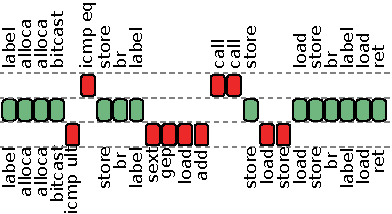
\includegraphics[scale=1]{Figures/FMSA_FunctionSA.pdf}
\caption{The sequence alignment between two functions, identifying the equivalent segments of code (green in the center) and the non-equivalent ones (red at the sides). Figure and caption taken from \cite{FunctionMergingSequenceAlignment}.}\label{fig:SequenceAlignment2Funcs}
\end{figure}

For this to work, criteria were chosen to determine when two instructions are considered to be matching. They are considered matching when they have semantically identical opcodes, equivalent result types and pairwise equivalent operand types. Types are considered equivalent when they can be bitcasted between each other losslessly.

In the final code generation stage, the aligned instruction segments with equivalent code are merged, while non-equivalent segments are maintained but guarded by a function identifier parameter that is added to the merged function.

% \begin{figure}[tbh!]
% \centering
% 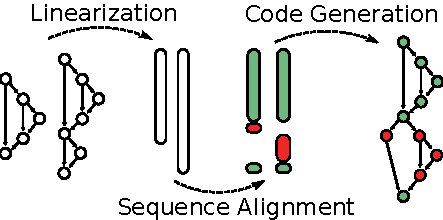
\includegraphics[scale=1]{Figures/FMSA_Technique.pdf}
% \caption{ Overview of function-merging by sequence alignment. Equivalent segments of code is represented in light green and the non-equivalent ones in dark red \cite{FunctionMergingSequenceAlignment}.}\label{fig:testsvg}
% \end{figure}

This technique demonstrated amazing results, reducing code size by 25\% on Intel architecture and 30\% on ARM. Approximately 2 times better than the state-of-the-art at the time.

\subsubsection{Alignment Score} \label{METRIC:AlignmentScore}
The sequence alignment between two functions is a property that identifies the structural similarity between two functions, serving as a key predictor of function merging profitability. This provides direct insight into how effectively two functions can be merged and is the characteristic our machine learning model aims to predict.
To quantify this value, the alignment score metric is used, defined as the ratio of the number of aligned instructions to the total number of instructions:
$$Alignment\ Score = \frac{Number\ of\ Aligned\ Instructions}{Total\ Aligned\ and\ Unaligned\ Instructions}$$
Using figure \ref{fig:SequenceAlignment2Funcs} we can calculate the alignment score as follows:
$$\frac{No.\ of\ Green\ Nodes}{Total\ No.\ of\ Green\ and\ Red\ Nodes}=\frac{14}{24} = 0.5833$$

Given that this metric is a ratio, this metric will be a continuous value in the range of [0, 1] inclusive, where 0 represents a completely dissimilar function pair and 1 representing a structurally identical function pair.


% \subsection{HyFM}
% HyFM is a notable function merging algorithm developed to solve the issue of the time needed to compiler code. Previous advanced function merging implementations were quadratic in complexity with regards to the number of functions. On top of that, the implementations were too keen on merging all selected functions, where most of the time the merged functions were unprofitable.\cite{HyFM:FunctionMergingForFree}

% \subsubsection{Basic Blocks}
% HyFM works at the basic block level, where basic blocks are blocks of instructions which are executed sequential, there are no branches. Since basic blocks are must shorter than functions, the alignment time is negligible compared to the time needed for attempting to align functions. By analysing how well basic blocks align with each other, the algorithm has an early sense of how well two functions align before attempting the alignment, saving time and resources from attempting unprofitable pairs.

% A fingerprint is generated for every basic block, and the basic blocks with the shortest distance between their fingerprints are considered good.
% If a pair of basic blocks are estimated to benefit from merging, it is then passes onto the more expensive merging phase.

% \subsection{Benefits}
% HyFM is able to decrease the alignment score

% \subsection{F3M: Fast Focuses Function Merging}

% \section{Quantifying Semantics}

% \subsection{Word2Vec}
% \subsection{IR2Vec}

\subsection{HyFM}
HyFM tries to tackle the inefficiencies of the previous state-of-the-art (SOTA) by introducing multiple optimisations \cite{HyFM:FunctionMergingForFree}. 

\subsubsection{Basic-Block Granularity} \label{HyFM:BasicBlockGranularity}
First, HyFM works at the basic-block level instead of function level. While the complexity is still $O(n^2)$ for the Needleman-Wunsch (NW)algorithm, $n$ in the previous SOTA refers to the number of instructions in functions whereas $n$ in HyFM refers to the number of instructions in basic blocks, which is considerably smaller, resulting in a dramatic memory reduction.

\subsection{Fingerprint} \label{HyFM:FingerprintDistance}
Before performing alignment, HyFM uses fingerprints to efficiently identify similar blocks. Each fingerprint is a fixed-size vector representing the frequency count of each opcode in a block. HyFM pre-computes fingerprints for all basic blocks and uses the Manhattan distance between these fingerprints to pair similar blocks from different functions. This lightweight filtering mechanism helps HyFM quickly focus on promising block pairs before applying the more expensive alignment analysis.


\subsubsection{Pairwise-Alignment (PA)} \label{HyFM:PairwiseAlignment}
Additionally, HyFM introduces a new linear-complexity pairwise alignment (PA) strategy that only aligns instructions in corresponding positions, with instructions matching only if they have the same opcode. It has been identified that most basic blocks that would be profitably merged have highly similar structure, making this simpler approach effective for real-world code. Finally, HyFM implements a multi-tiered profitability analysis, allowing it to bail out early from unprofitable and expensive merging attempts. This prevents wasting resources on generating merged code that would ultimately be discarded, contributing to HyFM's speedup compared to the previous SOTA.

\subsection{F3M: Fast Focused Function Merging}
This project is built on the current state-of-the-art function merging, Fast Focused Function Merging's (F3M) infrastructure. F3M represents the current state-of-the-art in function merging technology to address critical inefficiencies that previously made function merging impractical for large-scale applications. While its predecessor, HyFM, improved function merging by operating at the basic block level \cite{HyFM:FunctionMergingForFree}, F3M introduces fundamental innovations that dramatically reduce compilation time while maintaining or improving code size reduction.

The technique introduces two key innovations. First, F3M employs MinHash-based fingerprinting that better captures the semantic similarity between functions. 

\subsubsection{Min-Hash Fingerprinting} \label{METRIC: MinHashFingerprint}
Each instruction is encoded as a 32-bit integer representing four critical properties: opcode, result type, number of operands, and operand types. These encoded instructions are then grouped into overlapping "shingles" (pairs of consecutive instructions).  Multiple hash functions are then applied to each shingle, with only the minimum hash value across all shingles from each function retained, producing a fixed-length fingerprint vector.

\begin{figure}[h!]
\centering
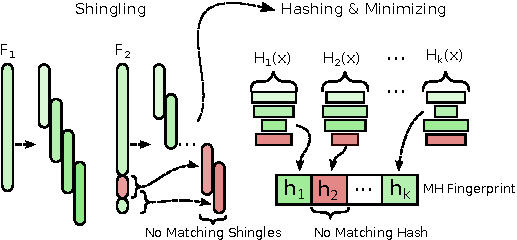
\includegraphics[scale=1]{Figures/F3M_MinHash.pdf}
\caption{The MinHash algorithm: Textual documents are broken up into overlapping subsequences; Each subsequence is hashed with k different hash functions; For each function, the smallest hash is saved creating a fingerprint of k entries. In this example, two functions differ in only a couple extra instructions inside F2. For F2’s fingerprint, this creates shingles and hashes with no matches in F1, representing the slight difference between them. Figure and caption taken from  \cite{F3M:FastFocusedFunctionMerging}.}\label{fig:testsvg}
\end{figure}

\subsubsection{Comparing MinHash Fingerprints} \label{METRIC:MinHashDistance}
To compare the MinHash fingerprints, the Jaccard Index between two fingerprints is calculated, representing the likelihood of matching instruction subsequences. For two fingerprints A and B, the index is calculated by finding the ratio of identical pairwise hash values compared to the total number of hashes ($k$):

$$J(A, B) = \frac{|A\cap B|}{k}$$

The Jaccard distance is then computed as: 
$$d(A, B) = 1 - J(A, B)$$

\subsubsection{Locality Sensitive Hashing (LSH)}
Second, F3M implements Locality Sensitive Hashing (LSH) to drastically reduce the search complexity from quadratic to near-linear. Rather than comparing every function against every other function, LSH divides each fingerprint into multiple bands (groups of hash values) and then maps each band to buckets in a hashmap. Only functions that share at least one bucket are considered for detailed similarity analysis, cutting down the amount of similarity analysis needed to be done.

% \begin{figure}[tbh!]
% \centering
% 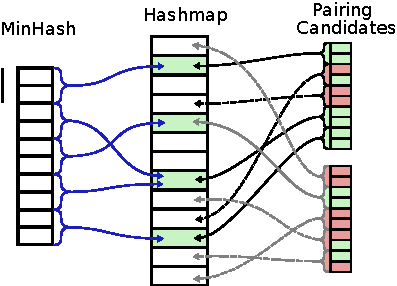
\includegraphics[scale=1]{Figures/F3M_LSH.pdf}
% \caption{ LSH - Similar sequences hashing to the same buckets. Three fingerprints
% with 10 hashes each, setting b to 5 and r to 2. References to each item are
% placed in each of their respective buckets. Since they share at least one of
% their bands they will be compared during candidate lookup \cite{F3M:FastFocusedFunctionMerging}.}\label{fig:testsvg}
% \end{figure}

\todo {INCLUDE SECTION/IMAGE ON HOW THE FUNCTIONS GET MERGED}


F3M was able to reduce the code size by a further $6\%$ on average while being able to reduce the compile time by $1.8\times$ on average across a wide range of benchmarks. Additionally, this shows the importance of the when-to-merge heuristics on the performance. Although F3M performs very well, especially for the amount of time needed to compile, the model is still very dependent on handcrafted heuristics that use fixed encoding schemes and statically determined parameters. These preset rules cannot adapt to different code patterns or contexts, and may not recognise all the patterns which indicate a suitable match.



\section{Machine Learning} \label{ML}
Machine learning (ML) offers an alternative by shifting from explicitly programmed rules to data-driven decision models. A machine learning model is a mathematical model with parameters that is tuned using data. The fundamental advantage of ML-based approaches lies in their ability to discover and leverage intricate patterns across multiple dimensions of code structure and behaviour.

\subsection{Supervised Learning}
There are multiple machine learning paradigms, each classified by the way they learn from their data and whether the expected output is provided.

Supervised learning is a machine learning paradigm in which learning is guided by labelled data \cite{MLParadigms} \cite{SupervisedLearningAndTrainingProcess}. In this approach, each input example is paired with a corresponding output, allowing the model to learn a mapping from inputs to outputs through the minimisation of a defined loss function. This process often involves iterative optimisation techniques to adjust model parameters and improve prediction accuracy. 

This supervised approach is more appropriate than alternatives like unsupervised learning, which typically operates by identifying similar data points through clustering or pattern recognition techniques. While unsupervised learning can identify similar functions, it is not quantify merging benefits.

For function merging optimisation, supervised learning enables a model to predict the profitability of merging two functions by training on examples of previously merged functions and their alignment score. In our context, the labelled data consists of pairs of functions and their corresponding alignment score.

\subsection{Loss Function} \label{ML:LossFunction}
A loss function, also known as cost or error function, is a mathematical function that quantifies the difference between the model's current predicted value and the ground truth (actual values).

Loss functions fall into two primary categories corresponding to the tasks, regression models (predicting values on a continuous spectrum) and classification models (selecting a value from a discrete set of values). For this paper we will be focusing on regression loss functions to predict the alignment score for a pair of functions, further discussed in section  \ref{METRIC:AlignmentScore}, allowing the estimate of merging benefits without expensive computations.

\subsubsection{Mean Squared Error (MSE)}
Mean squared error is a widely used loss function for regression tasks. It is derived by the following formula: 
$$MSE=\frac{\sum^n_{i=1}(y_i-\hat{y}_i)^2}{n}$$

\hspace{1cm} $y_i = $ Ground Truth Value

\hspace{1cm} $\hat{y}_i = $ Predicted Value

\hspace{1cm} $n = $ Number of Samples

The squaring operation in MSE provides two benefits. First, it makes all errors positive, ensuring that when multiple errors are combined and averaged in a batch, positive and negative errors do not cancel each other out, providing a true measure of error. Second, it emphasises larger errors due to the quadratic nature of the function. This emphasis prioritises the reduction of substantial prediction errors before fine-tuning smaller discrepancies—a desirable property when approximate predictions in the correct range, especially important when dealing with small values in the range of 0-1.

A smaller MSE is better, signifying reduced discrepancy between the predicted value and the ground truth. For our function merging application, MSE is preferable to alternatives like Mean Absolute Error (MAE) because the quadratic penalty helps the model focus on avoiding large prediction errors that could lead to poor merging decisions.

% \subsubsection{Mean Absolute Error (MAE)}

\subsection{Gradient Descent} \label{ML:Gradients}
The derivative of a function $f$, given by $\frac{df}{dx}$ measures the sensitivity of a function to change in the output given a certain input. This rate of change is also known as a function's gradient; geometrically, the slope of the tangent to the function's plot at a certain input. 

Gradient descent, the primary optimisation algorithm in deep learning, involves two stages, forward propagation and backward propagation. During \textbf{forward  propagation}, the model processes the training data through itself to produce a set of predictions. The loss function then quantifies the error between these predictions and the ground truth.

During \textbf{backward propagation}, the gradient for the loss function is calculated with respect to each parameter in the model using the chain rule. The gradients indicate the direction and magnitude of parameter adjustment needed to reduce the loss. Each parameter then is adjusted in the opposite direction of the gradient, scaled by the selected learning rate, discussed in section \ref{ML:LearningRate}.  This process iteratively navigates the parameter space toward a local minima of the loss function if it is well designed. In practice, finding a global minima is not always possible, so a well suited local minima is sufficient for predictions.

The objective of all gradient descent methods is to minimise the loss function, iteratively refining the model to make predictions that more closely match the ground truth.

% \subsection{Training}
% Learning is a process to acquire expertise or knowledge about a domain through experience and practice \cite{LearningDefinition1}\cite{LearningDefinition2}. The training process follows the following cycle \cite{DeepLearningGoodfellow}:
% \begin{enumerate}
%     \item \textbf{Forward Propagation}: The model processes a batch of input samples through it's layers using the current parameters.
%     \item \textbf{Loss Calculation}: The loss function quantifies the error between the model's predictions and ground truth.
%     \item \textbf{Backward Propagation}: The gradients of the model's loss is calculated with respect to its parameters using the chain rule.
%     \item \textbf{Parameter Update}: An optimisation algorithm adjusts the parameters in the opposite direction of the gradient to reduce the loss.
% \end{enumerate}
% This process is repeated until a stopping criteria is met.

\subsection{Hyperparameters}
A ML model usually has hyperparameters to configure. These are model parameters which are not learnt, and are configured before a model starts training. Unlike model weights which are optimised during training, hyperparameters control the learning process itself. They control how the model learns and behaves from the input data. A subset of the dataset, called the validation set, is usually set aside to tune the hyperparameters. Some of the most common hyperparameters are discussed below.

\paragraph{Epochs} \label{ML:Epochs} The epoch specifies the number of times the model trains using the entire training data. Setting a value that is too low may cause the model to underfit\footnote{\textbf{Underfitting} - When a model is unable to capture the underlying patterns in the training data, leading to poor performance on training and unseen data} to the training data, while a value that is too high may cause the model to overfit\footnote{\textbf{Overfitting} - When a model starts memorising the training data, capturing noise and irrelevant information instead of trying to learn the patterns associated with the data leading to poor generalisation on unseen data} to the training data, causing a drop in performance when evaluated against the validation set. One way to prevent overfitting due to excessive epochs is by implementing early stopping. Early stopping addresses this by monitoring the model's performance on the validation data, and halting training when the validation performance degrades, preventing overfitting.

\paragraph{Learning Rate} \label{ML:LearningRate} The learning rate determines the size of the step taken by the model for each training iteration. Selecting a large value means less time is needed for training, but the model may overshoot the global minimum and struggle to converge. On the other hand, if the learning rate is too small, the model will converge on a local minimum and not be able to leave it, thus not finding the optimal solution. Adaptive learning rate techniques like Adam can adjust the learning rate dynamically during training to improve the convergence.

\paragraph{Batch Size} \label{ML:BatchSize} The batch size specifies the number of training samples processed in each training iteration. The loss and gradient is averaged for all training samples in a batch. Selecting a suitable batch size is important, one too small will cause the model to not converge on the right direction as it will account for all the noise, one too big and it will require more memory for training and converge to a suboptimal solution.


\paragraph{Hyperparameter Optimisation} Since hyperparameters can greatly affect a model's training, it is important to find a suitable value for the model and task. There are multiple ways to do this, including manually running experiments or Bayesian optimisation. Bayesian optimisation works by constructing a probabilistic model of the objective function and using it to select the most promising hyperparameters to evaluate next. 

\subsection{Imbalanced Dataset}
In a perfect world, a dataset will have a similar amount of data samples for across the output data's range/spectrum, but this is not always possible. If no effort is taken to take into account the imbalance of the data samples, a model will learn to predict more of the dominant data samples. To mitigate this, sample weightings can be used, where it will scale down the loss for the dominant data points and scale up the loss for under-represented data points, this is known as \textbf{cost-sensitive learning (weighting)} \cite{ImbalancedDataset}. This ensures that the loss function will adjust the parameter in a reasonable manner without overfitting itself to predict more for the dominant data points.

% \subsection{Testing}
% Finally, another third subset of the dataset is set aside to evaluate the model's overall performance, known as the testing set. It is crucial that this set of data has not been used or seen at all by the model, so that the model's final evaluation can be unbiased on its ability to generalise to unseen data. The subsets of data that have been discussed so far, training, validation and testing should all be divided up at the start before model training to prevent data from training to be used for evaluation or vice versa. For regression tasks, mean-squared error (MSE), mean absolute error (MAE) and mean absolute percentage error (MAPE) are popular options. The MSE was selected as the metric because it emphasises larger errors, especially important when we are dealing with such small numbers and the MAPE is unable to deal with ground truth values that are 0 as division with 0 is not possible.

\subsection{Other Applications of ML in compilers}

% \subsubsection{Optimisation Selection}
% Optimisation selection determines which compiler optimisations should be applied to a program to achieve the best performance, code size, or other objectives. Compilers typically have dozens or hundreds of individual optimisation passes available, each with various parameters and settings. \todo{CITE Optimisation SELECTION}

% The challenge lies in deciding which optimisations to apply to a particular program, in what order, and with what parameters. Traditionally, compilers use predefined heuristics based on fixed rules established by compiler developers. However, these heuristics often fail to capture the complex interactions between optimisations and program characteristics across different architectures.

% Optimisation selection using machine learning has emerged as a powerful approach to automate compiler optimisations. MILEPOST GCC represents one of the pioneering efforts in this area, automatically adjusting compiler optimisation heuristics to improve execution time, code size, or compilation time \cite{OptimisationSelectionML}. The system collects program features and execution feedback and then uses this data to train models that predict optimisation strategies for new programs. This approach eliminates the need for expert hand-tuning of optimisation heuristics for each new architecture or program. Experimental results showed that MILEPOST GCC could reduce the execution time of the MiBench benchmark suite on the ARC processor architecture.

% The key innovation of this approach is that it replaces static, hardwired compiler optimisation decisions with data-driven models that can adapt to different architecture characteristics. This makes porting optimisation compilers to new hardware significantly more efficient, as the system automatically learns appropriate optimisation strategies rather than requiring manual recalibration.

% \subsubsection{Iterative Compilations}
% Iterative compilation is a technique that repeatedly compiles a program with different optimisation settings and evaluates the resulting performance to find the best configuration. Rather than relying on heuristics to determine the optimal optimisation strategy upfront, iterative compilation empirically explores the space of possible optimisations. \todo{CITE ITERATIVE COMPILATION}
% Iterative compilation traditionally requires extensive and repetitive fine-tuning to find optimal compiler optimisations, which creates a significant bottleneck in the development process. This challenge is addressed by applying active learning techniques to minimise the cost of iterative compilation \cite{IterativeCompilationWActiveLearningML}.
% The research demonstrated that traditional iterative compilation wastes substantial effort collecting redundant training data. Many of the performance measurements collected contribute little to the final optimisation heuristic. Their approach optimised both the selection of training examples and the number of samples per example using sequential analysis.

% By applying active learning principles, their methodology reduced training overhead compared to approaches with fixed sampling plans. The system determines dynamically whether additional samples are needed for a particular configuration based on the current model's uncertainty. This transforms what would typically take months of compilation and performance measurements into days, making machine learning-based compilation much more practical for real-world deployment.

% \subsubsection{Loop Vectorisation}
% Loop vectorisation is a compiler optimisation technique that transforms sequential loop operations to take advantage of modern processors' SIMD (Single Instruction, Multiple Data) capabilities. Instead of processing one data element per instruction, vectorisation allows a single instruction to simultaneously operate on multiple data elements. \todo{CITE LOOP VECTORISATION}

% Loop vectorisation is a critical compiler optimisation for modern SIMD-compatible architectures. NeuroVectorizer represents a significant advance in this area by using deep reinforcement learning to predict optimal vectorisation factors for loops \cite{LoopVectorisationML}.

% Traditional vectorisers in compilers like LLVM use fixed-cost models based on heuristics to make vectorisation decisions. These models struggle to accurately capture data dependencies, computation graphs, and instruction organisations. NeuroVectorizer takes a fundamentally different approach by employing a neural network that learns code embeddings directly from loop source code and then uses reinforcement learning to determine the optimal vectorisation and interleaving factors.

% The system achieved impressive results, showing performance speedup compared to the baseline LLVM vectoriser across various benchmarks. The reinforcement learning model proved particularly effective because it can learn complex patterns from code structure without requiring explicit feature engineering and can co-optimise multiple objectives like execution time and code size simultaneously.

% \subsubsection{Function Inlining}
% Function inlining is a compiler optimisation that replaces a function call with the called function's actual body. This eliminates the overhead of the function call mechanism (saving the registers, jumping to the function code, returning, and more) \todo{CITE Function Inlining}. MLGOPerf extends machine learning approaches to function inlining decisions in LLVM \cite{FunctionInliningML}.

% While MLGO (Machine Learning Guided Optimisation) previously focused on optimising code size with ML-based inlining, MLGOPerf specifically targets performance optimisation. The system employs two ML models: a primary reinforcement learning model that makes inlining decisions and a secondary model (IR2Perf) that predicts post-inlining speedup to generate rewards for training the RL agent.
% This two-model approach enables fast training without requiring the time-consuming execution of actual programs for each training iteration. Experimental results showed that MLGOPerf improved performance over LLVM's O3 optimisation level on SPEC CPU2006 and Cbench benchmarks. 
% Function inlining optimisation represents a particularly challenging problem due to the exponential growth of the optimisation space, making machine learning approaches especially valuable in this domain.

\paragraph{Optimisation Selection} Optimisation Selection focuses on determining which compiler optimisations to apply to a program to enhance performance, reduce code size, or meet other objectives. Traditionally, compilers have relied on fixed rule-based heuristics developed by compiler engineers to choose from a vast array of optimisation passes. However, with techniques like those used in MILEPOST GCC, machine learning models now collect program features and runtime feedback to automatically predict the most beneficial optimisation strategies, thereby replacing static rules with adaptable, data-driven decisions. This not only streamlines the optimisation process for various architectures but also reduces the need for manual tuning by experts \cite{OptimisationSelectionML}.

\paragraph{Iterative Compilation} Iterative Compilation tackles the optimisation challenge by repeatedly compiling a program with different settings and empirically testing the resulting performance. Instead of depending solely on predefined heuristics, this method explores a broader range of optimisation configurations to identify the optimal solution. The process is enhanced by active learning strategies which intelligently select training examples and adjust sampling dynamically based on the model's uncertainty. This adaptive approach dramatically reduces the time and effort required for extensive fine-tuning \cite{IterativeCompilationWActiveLearningML}.

\paragraph{Loop Vectorisation} Loop Vectorisation is a compiler optimisation that transforms sequential loop operations to exploit the parallel processing capabilities of SIMD hardware. Traditional vectorisers use fixed-cost heuristic models that may not fully capture the complex data dependencies and instruction patterns within code loops. In contrast, advanced approaches like NeuroVectorizer use deep reinforcement learning to predict the best vectorisation factors for loops. This method learns code representations directly from the source code, allowing it to determine more effective vectorisation and interleaving factors, which in turn leads to significant performance improvements over conventional heuristic models \cite{LoopVectorisationML}.

\paragraph{Function Inlining} Function Inlining is a technique that replaces a function call with the body of the function itself, thereby eliminating the overhead associated with calling a function. Recent advances, such as MLGOPerf, extend machine learning techniques to optimise inlining decisions. This approach leverages a two-model strategy: a primary reinforcement learning model for decision making and a secondary model to predict the performance gains from inlining. By doing so, the system efficiently optimises inlining, and has demonstrated improvements in performance on standard benchmarks compared to traditional inlining strategies \cite{FunctionInliningML}.

% \begin{itemize}
%     \item Optimisation Selection \cite{OptimisationSelectionML}
%     \item Iterative Compilation using Active Learning \cite{IterativeCompilationWActiveLearningML}
%     \item Loop Vectorisation \cite{LoopVectorisationML}
%     \item Function Inlining \cite{FunctionInliningML}
    
% \end{itemize}

\section{Neural Networks}
Neural networks represent a specialised and powerful class of machine learning models inspired by the structure and function of the human brain. While traditional machine learning approaches often rely on carefully engineered features and may struggle with complex, high-dimensional data, neural networks excel at automatically learning hierarchical representations from raw inputs.

The foundation of a neural network consists of \textbf{artificial neurons}, a mathematical function that mimics the basic behaviour of a biological neuron. Each artificial neuron receives one or more input signals, multiplies them by their corresponding weight, sum up the values, adds a bias term, and then passes the result through a non-linear activation function to produce an output signal.

% TODO: Add picture of artificial neuron

The overall architecture of a neural network is defined by how these neurons are arranged in layers: the \textit{input layer} accepts raw data, one or more \textit{hidden layers} perform successive transformations to extract increasingly abstract features, and the \textit{output layer} generates the final prediction. The complexity and performance of a neural network is largely influenced by its \textit{depth} (the number of layers) and its \textit{width} (the number of neurons per layer). Training is typically performed via optimisation algorithms like gradient descent and back-propagation, which adjust the network’s weights to minimise a loss function.

This automatic feature discovery and end-to-end learning process, which minimises the need for manual feature engineering, sets neural networks apart from traditional ML.

\subsection{Semantical Representations} \label{subsection:SemanticalRepresentations}
Machine learning models face a fundamental limitation when processing data, they operate exclusively on numerical values. This creates a significant challenge when working with symbolic or textual data, such as program code, natural language, or other structured representations. Since these algorithms rely on mathematical operations, inputs must be represented as numeric values or vectors; raw non-numeric data cannot be directly processed or learned from.

To overcome this limitation, the symbolic representations need to be transformed into a numerical representation which preserves it's semantic relationships and enable effective machine learning. Word embeddings serve as a prime example of this transformation, as they map words into dense, continuous vector spaces that capture semantic information.

Simple encoding techniques like \textbf{one-hot encoding}, where each unique symbol is assigned its own dimension in a vector space, fail to capture meaningful relationships between elements because all symbols are equidistant, so the encoding does not reflect any inherent similarity or dissimilarity between words. Moreover, as vocabulary size increases, one-hot encoding leads to extremely high-dimensional and sparse representations. This not only results in inefficient use of memory but also significantly increases the computational cost of training machine learning models \cite{DeepLearningGoodfellow}.

For instance, \textbf{word2vec} employs a shallow neural network with two primary architectures, the \textit{Continuous Bag-of-Words (CBOW)} model and the \textit{Skip-Gram} model \cite{Word2Vec}. In the CBOW approach, the network predicts a target word based on its surrounding context words, while the Skip-Gram model does the reverse by predicting context words given a target word. Both models learn embeddings by optimising the prediction task over a large corpus, ensuring that semantically similar words are located near each other in the resulting vector space. Similarly,  \textbf{GloVe}  was proposed as a method that leverages global word co-occurrence statistics to generate embeddings reflecting nuanced linguistic relationships \cite{GloVe}.

These embedding techniques enable machine learning models to effectively utilise the underlying semantics of the symbolic data to be able to predict on future tasks.

\subsubsection{IR2Vec} \label{subsubsec:IR2Vec}
IR2Vec is a framework that generates scalable, continuous embeddings for LLVM's Intermediate Representation (LLVM IR) \cite{IR2Vec}. Unlike traditional word embeddings that map natural language tokens into dense vector spaces, IR2Vec transforms programs and functions into vector representations by modelling the relationships among IR entities, such as opcodes, types, and operands using a translational embedding model, like \textit{TransE} \cite{TranslationalEncoding}.

This process begins by extracting relational information from the LLVM IR, which IR2Vec stores as a triplet ($<h, r, t>$). $h$ (head) represents an entity in the IR, $t$ (tail) represents another entity in the IR that has a relationship with $h$ and $r$ (relation) represents the relationship between $h$ and $t$. The triplets are then processed using a translation-based embedding model inspired by \textit{TransE}. The core idea of \textit{TransE} is that relationships should be represented by vectors such that sum of the relation vector $r$ with the head vector $h$ should approximate to the tail's vector $t$.
$$h+r\approx t$$

Relying on this concept, IR2Vec is able to build up the vector representations of the fundamental components of the IR (opcodes, operands, ...) known as \textbf{seed encoding}. These seed embeddings can then be used to build up a higher-level embeddings for higher-level program abstraction like instructions, basic blocks, functions and modules, referred to as \textit{Symbolic Encoding}.

IR2Vec offers an even richer embedding by incorporating the program's flow details, like the use-def chains and the reaching definitions, into the symbolic encoding, aptly named \textit{flow-aware encoding}. This allows the encoder to capture the program's operational semantics in addition to the syntactical information, facilitating more effective analyses and optimisations. 

\subsection{Activation Functions}
Activation functions are crucial in dense layers as they allow the network to learn non-linear relationships in the data. Common activation functions include ReLU (Rectified Linear Unit), sigmoid, and tanh, each offering different properties for gradient propagation and feature representation.
\todo{Double check this information}
\subsubsection{Sigmoid Activation Function}
\subsubsection{ReLU Activation Function}

\subsection{Layers}
In this section, the layers and techniques used by the paper will be discussed.
\subsubsection{Dense Layers}
Dense layers, also known as fully connected layers, are a fundamental building block of neural networks. In a dense layer, every artificial neuron is connected to every neuron in the preceding layer, creating a network of weighted connections. The number of neurons in a dense layer could also be treated as a hyperparameter to be tuned. A dense layer performs the following mathematical transformation:
$$y = \sigma(Wx+b)$$

\hspace{1cm}$x = $ Input vector from the previous layer

\hspace{1cm}$W = $ Weights matrix

\hspace{1cm}$b = $ Bias vector

\hspace{1cm}$\sigma =$ An activation function to introduce non-linearity

Dense layers are known for their powerful feature extraction abilities by learning complex patterns and relationships within data. They transform an input's representation into a more abstract representation. The primary advantages of dense layers include their flexibility in handling fixed-size vector inputs and their strong representational capacity. However, they can be parameter-intensive as the number of weights grows quadratically with layer width. For an input dimension of $n$ and output dimension of $m$, a dense layer requires $n \times m$ weights plus $m$ bias parameters.

This parameter intensity can lead to computational complexity and overfitting in deep networks, which is why dense layers are often used in combined with regularisation techniques, 

\subsubsection{Dropout Layer}
Regularization techniques seek to prevent overfitting by introducing controlled noise during training so that models learn representations that generalize beyond the training set. One of the most popular methods for neural networks is dropout, which directly alters the network's architecture during training instead of the usual modification of the loss function. 

At its core, dropout is very simple, each neuron in a layer is randomly deactivated on each training sample with probability $p$ (dropout rate). Equivalently, each neuron is kept with probability $q=1-p$ . During the forward pass, a binary mask $m$ of independent Bernoulli random variables is sampled and applied to the neurons, any surviving neurons are scaled by $\frac{1}{1-p}$ so that their expected value remains unchanged \cite{DropoutPaper}.

Normal neural layer's mathematical representation:
$$y = f(Wx + b)$$
After applying dropout:
$$y=f(Wx+b)\times \textbf{m}$$
There are two variants of dropout, the standard dropout which applies the scaling during inference, and inverted dropout which applies the scaling during training. Most modern frameworks use inverted dropout by default to simplify inference \cite{TensorflowDropout, PyTorchDropout}.

Typical choices for the dropout rate $p$ ranges from 0.2 to 0.5, although these values should be treated as hyperparameters and tuned for each task \cite{DropoutPaper}.

\subsubsection{Multi-Headed Attention Layers} \label{ML:AttentionMechanism}
Attention layers allow a neural network to focus on the most important feature for the current task. Not all parts of the input contribute equally to solving a problem, by learning which elements require more attention, the network can make more informed decisions. 

The attention mechanism takes in two inputs, the first input will attend to the second. There are two variants of attentions, \textbf{self-attention} where both inputs are the same so the sequence is attending to itself, or \textbf{cross-attention} where both inputs are different.

The attention mechanism starts with three learned weights used to create three vectors from the inputs, the query (Q) vector is created from the first input, and the key (K) and value (V) vectors are created from the second input. 

Then, it compares each query against all available keys to find how well each key matches the query by calculating the dot product of the pair. High-scoring pairs are given more attention while low-scoring pairs are given less attention or ignored. The scores are then put through a softmax function that converts each score into a probability. Then, the value vector is multiplied by the weight, and the elements are summed up to generate a weighted sum to produce the first input's new vector representation after attending to the second input \cite{AttentionIsAllYouNeed}.

The model then uses the newly attended vector for further processing and prediction. The error is calculated, and backpropagation is then used to update the weights to generate the Q, K and V vectors.

A multi-headed attention layer takes it one step further by having multiple attention layers in parallel to model different relationship aspects. This works by dividing the Q, K and V vector representations across the number of parallel attention mechanisms, each mechanism is known as a head. Each head works on its allocated portion of the Q, K and V values before being concatenated to form the final representation, which is typically projected back to the original dimension.

Despite its effectiveness, attention and multi-headed attention models come with higher computation costs than traditional mechanisms due to the attention mechanism's nature, where every element in the sequence must attend to every other element, resulting in a $O(n^2)$ complexity with respect to the input length \cite{AttentionComplexity}.



\subsection{Siamese Neural Network} \label{ML:SiameseNetwork}
Siamese neural networks, named after Siamese twins, are a class of artificial neural networks that process two inputs in parallel using identical sub-networks with shared weights to produce comparable output embeddings. The embeddings are then compared using a distance or similarity function to produce a value suitable for verification and matching tasks \cite{SiameseModelIntro}.

The architecture's key characteristic is the weight-sharing constraint between sub-networks, which ensures that similar inputs are mapped to nearby points in the embedding space while dissimilar inputs are mapped to distant points. Additionally, this ensures that the embedding is consistent across both inputs, enabling the model to generalise similarity judgements on unseen pairs.

Siamese networks have found wide applications in signature verification, face recognition, and image similarity assessment \cite{SiameseModelSignatureVerification, SiameseFacialRecognition, SiameseImageSimilarity} \todo{cite the different methods}. Their effectiveness stems from learning a discriminative embedding space rather than direct classification.

For measuring the similarity between embeddings, numerous metrics can be employed. In this paper, we focus on the following two:

\paragraph{Manhattan Distance}
The Manhattan distance, also known as the L1 distance, measures similarity by computing the sum of absolute differences between corresponding elements of two vectors. For embeddings $a$ and $b$ of dimension $n$, the distance is calculated using

$$d(a, b) = \sum^n_{i=1}|a_i - b_i|$$

This metric derives its name from the grid-like street layout of Manhattan, where the number of blocks measures distances travelled horizontally and vertically. Manhattan distance produces a value that increases with dissimilarity.
\todo{Put a picture for Manhatten distance}



\paragraph{Dot Product}
The dot product, also known as the inner product between two vectors $a$ and $b$, is computed as:

$$\sum^n_{i=1}a_i \times b_i$$

When used as a similarity metric in Siamese networks, the dot product measures the directional alignment and magnitude correlation between embeddings. A higher dot product indicates a more significant similarity. However, if only directional similarity is desired, the dot product is sensitive to vector magnitudes.


\chapter{Design, Methodology \& Implementation - 25\%}
% This chapter describes the design, methodology and implementation for this project, and the reasoning for the decisions taking throughout this project, connecting the information from the last chapter to this project.

This chapter ties the material from the previous chapter to this project by outlining its design, technique, and execution as well as the rationale behind the choices made along its course.

\section{General Design and Methodology}
Function merging is a powerful compiler optimisation technique that reduces code size by combining similar functions, but its effectiveness depends heavily on identifying which function pairs are suitable candidates for merging. Current heuristic-based approaches often miss opportunities for optimisation or waste compilation time attempting to merge incompatible functions. This project aims to improve function merging in compilers by leveraging machine learning to predict function pairs that are likely to produce beneficial merges.

For this approach to succeed, comprehensive training data needs to be collected consisting of diverse function pairs and their merging performance. These functions will be encoded into a vector representation using IR2Vec to quantify the function's semantic meaning and multiple merging scores which are calculated by F3M's artifacts are contenders for quantify the merging performance. The collected data will require some processing to normalise before being used to develop, train and evaluate different ML models. The training process will involve feeding these vector representations into a neural network architecture that can effectively compare function pairs' encodings and predict their merging compatibility to improve the compiler's function merging decisions.

The project methodology is structured around three interconnected stages: data collection, machine learning model development, and integrating everything together.

The first stage involves collecting data, since effective machine learning benefits from representative data. This involves gathering two essential components: a suitable vector encoding of functions that captures their semantics and a metric that quantifies the similarity between function pairs to determine whether merging would be beneficial. \todo{Talk about the merging outcomes of F3M as well: Successful merges, new merged function size}.

In the second stage, various machine learning architectures are explored and fine-tuned using the collected data to evaluate their performance in predicting merge suitability. This experimentation allows us to identify the most effective model architecture for function merging.

In the final stage, the trained models and function encodings are integrated into the LLVM compiler and evaluated on a suite of benchmarks to measure it's performance in terms of code size reduction of the overall system.

The subsequent sections elaborates on each stage of this process, providing insight into the design decisions and implementation details. Furthermore this project also includes artefacts for reproducing results, including a set-up script to facilitate easy set up which will be detailed at the end of this section.

This project also includes artifacts for reproducing results, including a set up script which will be detailed in the subsequent sections along with elaborations on each stage of this process, providing insight into the design decisions and implementation details.

\todo{Include image of the overall pipeline of the project.}

\section{Data Collection}
To collect the function merging data, the previous SOTA function merging implementation, F3M, was executed on a suite of benchmarks: cc1plus, chrome, libreoffice, linux, llvm, Spec2006, and Spec2007 which were provided in F3M's artefacts as LLVM bitcode (\ref{LLVM:Bitcode}).

\subsection{Use of IR2Vec} \label{subsection:UseOfIR2Vec}
As mentioned in Section \ref{subsection:SemanticalRepresentations}, it is important to encode functions in a way that accurately captures their underlying semantics. To accomplish this, \textbf{\textit{IR2Vec}} was employed to transform the intermediate representation (IR) of each function into a 300-dimensional vector embedding. This wider dimensionality allows the encoder to capture more detail for each function and this process also produces a distinct embedding for every individual function making it a perfect fit for our needs to work at function-level granularity.

IR2Vec was selected for this project because of its proven ability to capture both the semantic meaning and flow of LLVM IR through flow analyses.\cite{IR2Vec}. Its efficient encoding process and graceful handling of out-of-vocabulary tokens via seed embedding vocabulary further contribute to its appeal as an encoder. Moreover, IR2Vec is fully open-source, facilitating straightforward customisation and extension. Furthermore, IR2Vec is available across multiple platforms, it can be utilised as a Python library, a C++ library, or even as a stand-alone binary. This flexibility ensures seamless integration into various development environments, simplifying the overall implementation of the project.

\subsection{Database Solution}
Prior to collecting any data, it was necessary to determine a suitable storage solution which fits the project's needs.

\paragraph{SQL vs CSV} \textbf{\textit{SQL}} databases offer significant advantages over simple file structures like \textit{CSVs} primarily due to the expressive power of the SQL query language. Rather than reinventing the wheel each time a complex query is required, SQL provides a rich set of built-in functions and operators for users. This expressiveness not only simplifies the process of querying but also enhances performance, especially when working with large volumes of data, by leveraging optimised indexing and storage mechanisms. Furthermore, the relational nature of SQL databases, where data is organised into interconnected tables, enables more efficient modifications and queries across related data sets, reducing redundancy and improving maintainability.

\paragraph{SQLite vs PostgreSQL} \textbf{\textit{SQLite}} was selected over other SQL solutions, such as \textit{PostgreSQL} primarily for its ease of use and minimal configuration requirements. Unlike PostgreSQL, which typically requires extensive setup, including robust security configurations and server management, SQLite operates as a server-less, file-based database, making it an ideal choice when sensitive data is not a concern. Additionally, SQLite provides a C++ interface, which is the language used to build LLVM and F3M. Finally, its widespread adoption in the Python ecosystem offers an advantage, popular libraries like \textbf{\textit{Pandas}} and \textbf{\textit{TensorFlow}} provide support to read data from SQLite directly, further simplifying the project's implementation by enabling straightforward connections and interactions.

\subsection{Database Design} \label{subsection:DatabaseSchema}
The design of this database schema is guided by the need to efficiently store and query data, especially since the number of function pairs scales quadratically to the number of functions in a program.

\begin{figure}[tbh!]
\centering
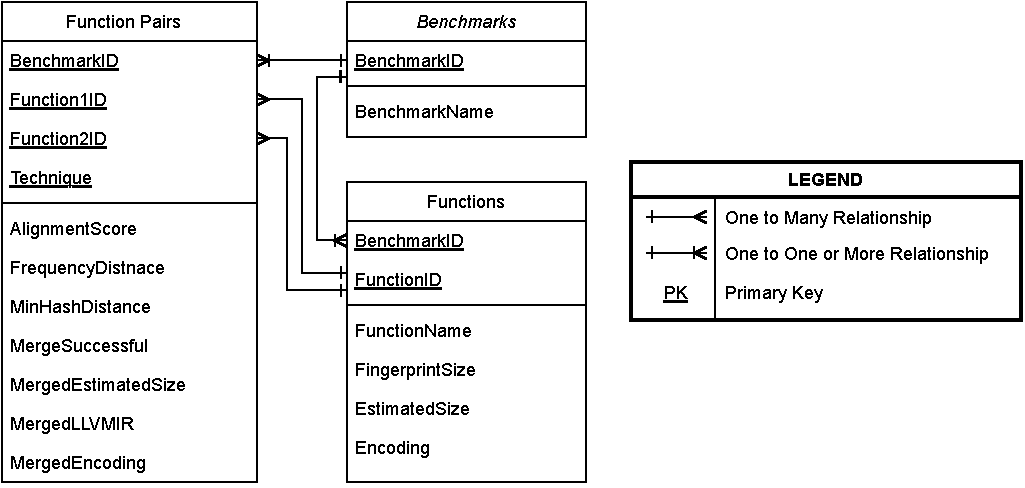
\includegraphics[scale=0.85]{Figures/DataCollectionSchema.pdf}
\caption{Schema of database used to store collected data using crows foot notation}\label{fig:DatabaseSchema}
\end{figure}


The schema consists of three primary tables, as illustrated in Figure \ref{fig:DatabaseSchema}. The \textbf{Benchmarks} table serves as the top-level reference point for all data points. This design ensures that each dataset being evaluated is logically isolated, facilitating independent analyses, comparisons, and debugging if needed.

The \textbf{Functions} table captures detailed information about individual functions for each given benchmark. Combining \textit{BenchmarkID} and \textit{FunctionID} as composite keys ensures that function identifiers are scoped locally within each benchmark, preventing cross-function ID collisions. The foreign keys ensure that each function entry is associated with a valid benchmark. All metadata fields remain optional to support flexible, use‑case‑driven data collection.

For each function, the function's name is recorded as a unique key for linking F3M outputs to IR2Vec embeddings. The fingerprint size is computed as the sum of the frequencies of opcodes in HyFM's function fingerprints, as described in section \ref{HyFM:FingerprintDistance}. Function size is then estimated by summing LLVM’s per‑instruction code‑size costs, queried via the TargetTransformInfo interface.

The functions' encoding are stored as BLOB type to store a pickled Python list representing the function's vector encoding. This decision aims to reduce redundant data transformations since the encodings are generated and used in Python (during training), storing them directly in binary format avoids unnecessary conversions and parsing to and from string representations.

Finally, the \textbf{FunctionPairs} table stores all function pair comparisons. The foreign keys ensure that referenced benchmarks and functions exist. This table only uses a single BenchmarkID alongside two function IDs because function merging is only performed within the same program. This table also stores the distance metrics, AlignmentScore (\ref{METRIC:AlignmentScore}), FrequenceDistance (\ref{HyFM:FingerprintDistance}), MinHashDistance (\ref{METRIC:MinHashDistance}) and merging outcomes. The merging outcomes are optional fields, as if a merging attempt fails, there is no merged function to get information from.

\subsection{Data Collection Framework}
The data collection step was split into two steps, one to collect F3M's merging attempts information and one to collect the functions' embeddings from IR2Vec.

For both steps, two automated scripts were made for each step, where they both share a lot of similarities. A base directory of the benchmarks would be specified by the user, and the script would dive into the directory and sub-directories looking for $\_main\_.\_all\_.\_files\_.\_linked\_.bc$ files, which are bitcode files for the benchmarks. For each bitcode file, the benchmark's name is determined by examining the name of its parent directory. The scripts also has an additional input to specify the database's name and path, ensuring that different runs remain separate if the user wishes to keep them organised. Moreover, the parameters allow multiple shell sessions to run the same script concurrently on different benchmarks, enabling several benchmark data collections to occur simultaneously. This concurrent execution saves time since each script processes benchmarks sequentially. Additionally, this design prevents the corruption of a single SQLite file, as the scripts do not incorporate concurrency controls for simplicity.


\subsubsection{Collecting F3M Merging Metrics}
The collection of merging metrics was intended to be done before collecting function encodings, since not all functions touched on by IR2Vec would be merged in F3M.

To collect merging metrics, SQLite's C++ interface had to be integrated into F3M's implementation within the LLVM codebase. Initially, a SQLite database is initialised with the user-specified name, and F3M's reporting feature is repurposed to pipe the pairwise metrics into the initialised database instead of the terminal.

After obtaining the benchmark name and bitcode file location for each benchmark from the script mentioned above, the script changes its working directory to the bitcode file's directory and executes a \textbf{\textit{make}} command to run each benchmark using F3M's binary, passing the benchmark's name to the compiler via environment variables.

After running the scripts from this step, all fields in the new database should be populated except for the encoding field, which will be populated in the next step.

\subsubsection{Collecting IR2Vec Function Encodings}
The function encodings collection was segregated into a separate step because function encodings only need to be collected once per function, whereas the merging metrics collection processes each function quadratically.

After locating each benchmark's bitcode file using the script mentioned above, IR2Vec's binary was used to generate function-level embeddings from the bitcode files, which were then stored in a text file.

Then the script opens the text file and loads the embeddings into a Python dictionary, with the keys being the function names and the values being the embeddings, parsed into Python lists and serialised into a binary object using the Python Pickle library.

Next, using the database path and the benchmark name, the IR2Vec collection script accesses the database and retrieves the benchmark ID corresponding to the benchmark name, along with all associated function IDs and their function names. These retrieved function names are then matched with the function encodings generated by IR2Vec. Using this matched information, the relevant embeddings are extracted from the dictionary and inserted into the database.

During this process, an issue was identified: the function names used by IR2Vec and LLVM were different. Specifically, LLVM's function retrieval returns mangled names, while IR2Vec produces demangled names. Consequently, IR2Vec's source code was modified and rebuilt to conform to LLVM's naming convention.

\todo{Show an example of before and after of modifying IR2Vec's codebase}

\subsubsection{Merging Data}
Due to the fact that multiple scripts could be run concurrently while writing to different databases, there is a need to merge all data into a single, centralized database. The script accepts a variable number of arguments specifying the input databases to combine and an argument for the new database's name. It works by initialising a new database using the specified name, connecting it to each of the existing databases, and then copying over the information.

\section{Model Development}
To develop machine learning models, the data from the previous step are pre-processed and partitioned to form a representative dataset. Then, two model architectures were designed based on carefully considered rationale. Finally, a framework was established to support efficient training, testing, fine-tuning, and evaluation of these models, streamlining experimentation and providing a reliable structure for iterative improvements.

\subsection{Data Pre-Processing}
\subsubsection{Data Imbalance} \label{Design:DataImbalance}
A major challenge encountered with the dataset was the overwhelming number of function pairs with an alignment score of 0. In total, there were \textbf{\textit{2.2 billion}} function pairs collected, of which \textbf{\textit{1.67 billion}} samples had an alignment score of 0 (zero-samples), \textbf{\textit{1.7 million}} had an alignment score of 1 (one-samples) and \textbf{\textit{570 million}} has an alignment score between 0 and 1 (non-zero-non-one samples). If this imbalance is not properly addressed, the model would likely learn to predict 0 for most situations to achieve a superficially low error, but produces unhelpful predictions.

This imbalance is mitigated in two ways. First, a large portion of the zero samples is discarded so that the number of remaining zero samples equals the combined total of one samples and non-zero-non-one samples. This balancing strategy reduces the dominance of zero samples and decreases overall training time by lowering the total number of training examples. After this step, the following condition holds true:
$$Zero\ Samples = One\ Samples + Non\_Zero\_Non\_One\ Samples$$

Secondly, during model training, each remaining zero-alignment sample is assigned a weight of \textbf{\textit{0.001}}. This weighting means that every non-zero alignment sample contributes 1,000 times as much to the loss function as a zero-alignment sample, thus diminishing the influence of the overly abundant zero samples. In this way, the model is incentivised to learn accurate predictions for non-zero alignment scores.


\subsubsection{Data Split} \label{Design:DataSplit}
After collecting and processing the data, we end up with \textbf{\textit{1.1 billion}} function pairs. The order of data is then randomised to make it diverse when encountered by the machine learning model. After which the dataset is split into three smaller SQLite datasets, the training, validation and testing datasets, each making up 70\%, 10\% and 20\% of the pre-processed dataset respectively. The training dataset is used by the model to train itself, while the validation set is used by the model to tune its hyperparameters (discussed in section \ref{subsubsection:HyperparameterTuning}) and the test set is then used to test the model's performance on unseen data.

Pre-splitting the dataset accelerates training by eliminating the need to determine the data split during runtime. Furthermore, maintaining a permanent split throughout the model development stage reduces uncertainty in performance evaluations, as the deterministic nature of the split ensures consistent results, consequently any changes in metrics could be mainly attributed to the model's performance.

\todo{Add a bar graph of the frequence of the values in the dataset}

\subsection{Hyperparameter Tuning} \label{subsubsection:HyperparameterTuning}
% \subsubsection{Hyperparameter Tuning} \label{subsubsection:HyperparameterTuning}
Due to the sheer volume of training data available, tuning the hyperparameters using the entire training dataset would be computationally prohibitive. Therefore, a subset of 300 million training samples is used for the hyperparameter tuning stage. During this phase, a dedicated validation set is employed to evaluate each configuration of hyperparameters, ensuring that the model’s performance is robust and generalises well, not overfitting to the training data. Once the optimal hyperparameters are identified through this procedure, the model will be retrained on the full dataset comprising 1.1 billion training samples using these optimal settings.

For the hyperparameter optimisation, \textbf{\textit{Optuna}} is employed. Optuna is an efficient, automatic hyperparameter optimisation framework that utilises Bayesian optimization methods to navigate the hyperparameter space. Each evaluation of a particular set of hyperparameters is referred to as a \emph{trial}. During each trial, the model is trained on the subset of data, and its performance is measured on the validation set, specifically its mean squared error. The results from numerous trials guide the search process, balancing exploration of new configurations and exploitation of known good regions in the hyperparameter space, ultimately converging towards a trail with the lowest mean squared error with the optimal settings.

\subsection{ML Model Design}
In general, the machine learning model developed will take in two function's embeddings as inputs and produce an alignment score as the output.

The alignment score provides a robust distance metric for function merging by capturing the structural and semantic correspondence between code sections, discussed in section \ref{METRIC:AlignmentScore}. The alignment-based approaches excel at detecting semantically equivalent code regions despite variations in the implementation. Furthermore, the score gives an early insight into the potential code size reduction achieved through merging the function pair as it measures how well two functions overlap. 

\subsubsection{Dot Product Siamese Model}
This is an implementation of the Siamese network discussed in section \ref{ML:SiameseNetwork}, which uses a shared encoder to process two function encodings and then comparing them using a dot product similarity.

\paragraph{Shared Encoder} The shared encoder is used to produce embeddings for both inputs within the same feature space, transforming the IR2Vec's embeddings into an embedding that facilitates the comparison of the generated embeddings by dot product.

The shared encoder first expands IR2Vec's 300-dimensional vector in 512 dimensions to try and capture any more semantics that was lost due to the limited amount of elements, followed by a dropout layer with a dropout rate of 16.6\% to prevent overfitting. Then a dense layer compresses the new 512 dimensions into 128 dimensions to abstract and keep the most relevant information for the comparison task.  Then batchnormalisation is used to <reasoning> and using this means one less hyperparameter to training compared to using a regular normalisation layer.

The dot product of the two new embeddings are calculate before passing it to a dense layer of 1 unit with a sigmoid layer to map the dot product to a 0 or 1 range to match the alignment score's range.

The shared encoder is used to produce embeddings for both inputs within the same feature space, transforming the IR2Vec's embeddings into a more comparable representation that enhances the comparison of function pairs by dot product.

The shared encoder first expands IR2Vec's 300-dimensional vector to 512 dimensions to capture richer semantic information that might be constrained in the original representation, followed by a dropout layer with a dropout rate of 16\% to prevent overfitting. Then a dense layer compresses the expanded 512 dimensions into 128 dimensions to abstract and keep the most relevant information for the comparison task. 

After this, batch normalisation is applied to standardise the layer outputs, which helps stabilise and accelerate the training process by reducing internal covariate shift. Using batch normalisation also reduces the need for careful initialisation and allows higher learning rates, effectively requiring one less hyperparameter to tune compared to using a regular normalisation layer.

\paragraph{Score Generation}
Once both function embeddings have been processed through the shared encoder, their dot product is calculated to measure the similarity between them, capturing how aligned the two functions are in the embedding space. This similarity value is then passed through a dense layer of 1 unit with a sigmoid activation function to map the dot product to the [0,1] range, corresponding to the desired alignment score range.

\subsubsection{Multi-headed Self-Attention Model}
This is an implementation of a model which tries to take advantage of the attention mechanism discussed in section \ref{ML:AttentionMechanism}.

The model first processes each IR2Vec 300-dimensional embedding through a shared dense layer with 512 units and ReLU activation, expanding the representation to capture richer semantic information. Unlike the Siamese model, these expanded representations are then reshaped and concatenated to form a sequence of two tokens, allowing the model to treat the function pair as a unified sequence.

The core of this architecture is the transformer encoder block, which implements multi-head self-attention with 4 attention heads, each with a dimension of 64. This mechanism allows each function representation to attend to the other, capturing complex relationships between their features. 

The self-attention output passes through dropout (30\%) to prevent overfitting and uses skip connections and layer normalisation to stabilise training. The subsequent feed-forward network with ReLU activation further processes these attention-weighted representations through a dimension of 64 before returning to the original dimension. After the transformer encoding, the model applies global average pooling to aggregate the sequence information into a single vector representation. This condensed representation is then passed through a final dense layer with sigmoid activation to produce an alignment score in the [0,1] range, where higher values indicate better candidates for function merging.

By leveraging attention mechanisms instead of simple dot products, this model can potentially capture more nuanced relationships between function pairs, learning which aspects of functions are most relevant for aligning functions.


\subsection{Framework/Pipeline for Model Development}
This section discusses the framework design and explains key design decisions.

\subsubsection{Serialising Data}
Initially, the models loaded data using Tensorflow's dataset interface which acts as a lazy iterator, querying the SQLite dataset. Tensorflow's SQL dataset interface could not be used, because the encodings which were stored as BLOB objects required depickling before being loaded into the model.

Direct querying of the SQLite dataset proved extremely slow. Therefore, with assistance from my supervisor, Pavlos, a script to serialise the data into \textbf{\textit{NumPy}} arrays was created. This approach significantly reduced the number of processing operations required, resulting in faster loading and processing times compared to SQL querying.

The serialisation utilises two two-dimensinal \textit{NumPy} arrays: one to store function encodings and another to store alignment scores. For the encodings array, each unique tuple (BenchmarkID, FunctionID) is assigned a new unique function ID. These function IDs are stored with their respective encodings occupying the remaining columns.

The second array stores alignment scores of function pairs using three columns: the first function's unique ID, the second function's unique ID, and the pair's alignment score. Without formal measurements, this method was observed to decrease training time by approximately 60\% in small test cases.

The \textit{NumPy} arrays are saved to binary files for direct loading when needed. While the number of functions is manageable, it pales in comparison to the number of function pairs. Therefore, the array storing pairwise metrics must be split into multiple binary files of specified number of points while the array storing function encodings can be contained in a single file.

Selecting an appropriate chunk size during serialisation is crucial, as excessively large values can cause system crashes. The script verifies that at least 20\% of system memory is available before retrieving the next data batch. If insufficient memory is available, the script sleeps until adequate memory becomes available. A potential deadlock can occur if the script holds data in memory while waiting to meet chunk size requirements but lacks sufficient memory to retrieve the additional data needed.

\todo{ADD A PICTURE OF THE SERIALISED DATA}

\subsubsection{Loading Data}
This process utilises the TensorFlow dataset interface, where the dataloader first loads all function encodings into memory by storing them into a \textit{Python} dictionary, then processes each chunk of pairwise metrics by replacing unique function IDs with their corresponding encodings.

This loading process was observed to be time-intensive. To address this performance bottleneck, the \textbf{\textit{concurrent}} Python library was implemented to load the next data chunk in a separate thread while the model trains on the current available data. These loaded chunks are placed in a queue which the dataloader lazily iterates through, significantly reducing the time the model spends waiting for data preparation between chunks and thereby accelerating the training process.

The data loader is configured to process only one additional file concurrently, as processing more files simultaneously provides no performance benefit and consumes excessive system memory. This is particularly important since each fully expanded input contains 601 32-bit float values, around 2KB (\ref{Calculation:InputSize}).

To prevent system crashes due to memory exhaustion, the loader verifies that at least 20\% of system memory is available before loading and expanding each new data chunk. This memory management strategy ensures stable operation throughout the training cycle.

\subsubsection{Running the Model}
To steamline the process of model development, a centralised script was developed that efficiently handles both training and hyperparameter tuning across different model architectures. The main script accepts various command-line arguments to specify the model type, the operational mode (training or hyperparameter tuning), the location to saved the trained models to and when in training mode, the specific model parameters.

For this modular approach to function effectively, each new model must implement two standard interface functions: $get\_model()$ and $HyperParameterTraining()$. The $get\_model()$ function provides the main script access to the model, while $HyperParameterTraining()$ encapsulates any model-specific hyperparameter optimisation requirements. This standardized interface eliminates redundant code and significantly simplifies working with different model designs.

For model evaluation and result visualisation, a \textbf{\textit{Jupyter Notebook}} was created. This notebook tests trained models against the test dataset, calculates the mean squared error, and generates comparative plots of predicted versus true alignment scores to visually demonstrate model performance.

\section{System Integration}
This section describes how IR2Vec and the trained ML models were integrated into the F3M's codebase to leverage the ML model's heuristics for function merging decisions.

\subsection{Integrating Tensorflow}
The initial integration strategy involved using \textbf{\textit{PyBind}} to load the trained TensorFlow models into the compiler. This approach was selected because one variant of the Siamese Model had been developed using the L1 distance metric instead of the dot product. Since this implementation required a custom layer not natively available in TensorFlow, PyBind appeared advantageous for running python code, therefore allowing the use of custom layers.

However, PyBind consistently crashed when attempting to load TensorFlow models. Given these limitations, \textit{TensorFlow's C++ API} was adopted as an alternative solution for loading the trained models. This decision required abandoning the L1 distance Siamese model due to the engineering work required to support its custom layer in the new integration approach.

\subsection{Integrating IR2Vec} \label{Design:IntegratingLLVM}
Next, since IR2Vec was developed in C++, the initial approach involved incorporating its header files and source code from the official \textit{GitHub} repository. However, while testing the project, errors occurred whenever the compiler attempted to request embeddings from IR2Vec. This compatibility issue likely stemmed from version differences between the LLVM versions used by each project. IR2Vec was based on LLVM 18.1.8 at the time of this project, while F3M used version 18.0.0, necessitating an alternative solution.

The adopted workaround involved pre-generating function encodings using IR2Vec's stand-alone executable for the benchmarks and storing them in text files. During compilation, the system would then only need to parse these files and load the encodings into a map for quick encoding lookup of each function.

This integration approach imposed a significant limitation: newly generated merged functions could not be considered as candidates for further merging, as it was not possible to obtain embeddings for these new functions during compile time. This constraint restricted the optimisation potential to a single pass of function merging.

\subsection{How it all fits together}
The function merging process begins when all candidates are placed into a priority queue. As each candidate is processed, it is removed from the queue for assessment. The queue prioritises functions with larger fingerprint sizes, giving them precedence over smaller ones. During assessment, the system predicts the alignment score between the current function and all other candidates in the queue. Merging is then only attempted with the function that yields the highest predicted alignment score.

\paragraph{Thresholding Alignment Score} Not all highest predicted score functions are merged, only if the alignment score is higher than a pre-determined threshold value. This was added because a function could be unsuitable to merge with all other functions, and we would like to skip it instead of wasting compiling time on unprofitable merges. Multiple thresholding values were tried, 0.4, 0.5, 0.6.

\paragraph{Thresholding Alignment Score} Even when a highest-scoring function pair is identified, merging only proceeds if the alignment score exceeds a pre-determined threshold value. This threshold mechanism prevents wasting compilation resources on unprofitable merges when a function may be unsuitable for merging with any other functions in the queue. During system evaluation, multiple thresholding values were tested, including 0.4, 0.5, and 0.6, to determine the optimal balance between merge opportunities and compilation efficiency.

% \section{Artifactory and Set up Script}
% \subsection{Talk about the set up script provided}
% Discuss the artifact being available and the simple set up script. Explain why IR2Vec has to be built individually by the user.

\section{Artifactory and Set up Script}
\subsection{Repository and Accessibility}
All code developed for this project is publicly available as artifacts in a GitHub repository, linked in appendix \ref{Artifacts}. This repository contains the complete codebase, including models, data processing scripts, integration components, and evaluation tools. The repository is structured to facilitate easy navigation and understanding of the project's components, with clear documentation for each module.

\subsection{Automated Setup Script}
To enhance accessibility and reproducibility, a comprehensive setup script has been developed that automates the installation and configuration process. The script applies custom configurations to ensure compatibility between components and prepares the system for immediate experimentation. This automation significantly reduces the technical barriers to reproducing the research, allowing users to quickly begin exploring the function merging improvements.

A detailed README file is included in the repository root, providing comprehensive guidance through the project setup process. The documentation clearly outlines the required dependencies, and tested environments to ensure compatibility. It includes straightforward installation instructions that walk users through the cloning process and execution of the setup script.

The setup script intentionally excludes the complete installation of IR2Vec, instead only cloning the repository and applying necessary patches. This decision was made because IR2Vec requires a local build of LLVM as a prerequisite, which would require extensive disk space and compilation time.














\chapter{Result - 25\%}

\chapter{Evaluation}
In this section, this project will be evaluated according to three criteria introduced in section \ref{section:aims}. First, the trained models' performance on the test set is analysed. Second, all merge attempts are examined for their profitability to evaluate the quality of the merge attempts. Third, the size of the code is measured to assess the impact of merging on the code footprint.

\section{Experimental Set Up}
The following experiments were run on an Intel Xeon Gold 6338 CPU with 128 threads and two Nvidia A10 GPUs running AlmaLinux. The results are reported on the SPEC CPU 2006 and SPEC CPU 2017, presenting individual benchmark outcomes. Since F3M is non-deterministic, the results are averaged over three runs.

\section{ML Model Prediction Accuracy} \label{Eval:MLAccuracy}
To assess the trained deep learning models' prediction accuracy, the models are evaluated against a test set of \textit{228 million} unseen samples. We quantify the performance of the models using TensorFlow's built-in evaluation feature, which computes the mean squared error (MSE) between each prediction and its true value. MSE is a standard metric for evaluating and comparing regression models in machine learning. Furthermore, a heat map is generated to visualise the model's performance, plotting the model's predicted alignment score against the true label to visualise the model's performance.

Given the data imbalance (\ref{Design:DataImbalance}), two MSE values are calculated, one using the whole test set and one using only non-zero samples from the test set. This approach addresses bias compensation, the imbalanced dataset might inherently bias the model toward predicting lower alignment scores, and the separate MSE helps quantify whether the model successfully overcomes this training bias. Additionally, this helps us quantify the model's performance for functions where there are similarities between them, as this is more important for our purposes.

\subsection{Dot Product or Cosine Similarity}
During the model selection process, two variants of the Siamese neural network were designed and evaluated, one using the cosine similarity and another using the dot product as the similarity metric. A subset of approximately \textit{80 million} training samples was used for initial model evaluation to efficiently determine the most promising architecture before proceeding to hyperparameter tuning and training on the full dataset.

Scatter plots showing predicted alignment scores against actual alignment scores were generated to compare the models' predictive capabilities. These visualisations excluded data points with a true alignment score of 0 to focus specifically on the models' ability to predict non-zero alignment values. Both models were trained with identical hyperparameters for six epochs each, the only difference being the similarity metric used.

\begin{figure}[tbh!]
\centering
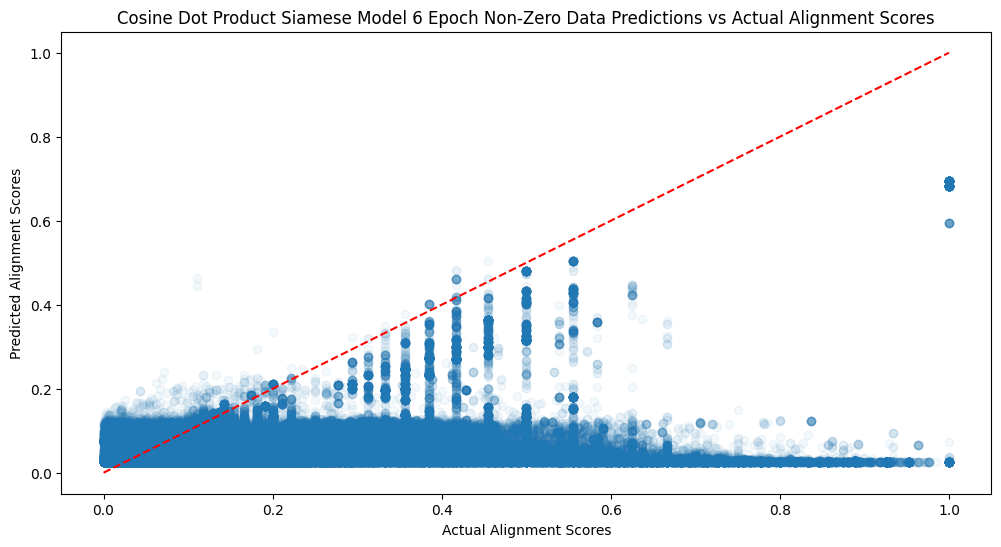
\includegraphics[scale=0.4]{Figures/ModelArchitecture/Cosine6Epoch.png}
\caption{\textbf{Scatter Plot of Cosine Similarity Siamese Model's Predictions vs. True Labels} using 80 million training samples. The diagonal line represents perfect agreement. Scatter plots effectively reveal patterns in smaller datasets; however, they lose clarity as datasets grow larger. In the subsequent sections, the volume of data is significantly larger, so heat maps were used to capture density and trends better.} 
\label{fig:CosineSiameseModel}
\end{figure}

\begin{figure}[tbh!]
\centering
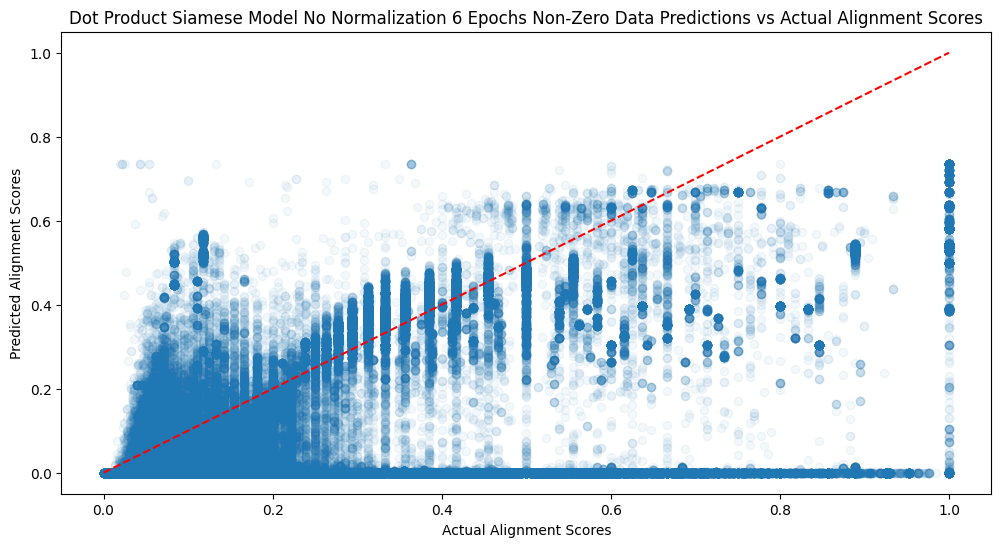
\includegraphics[scale=0.4]{Figures/ModelArchitecture/DotProdArchitecture.png}
\caption{\textbf{Scatter Plot of Dot Product Siamese Model's Predictions vs. True Labels} using 80 million training samples. The diagonal line represents perfect agreement. Scatter plots effectively reveal patterns in smaller datasets; however, they lose clarity as datasets grow larger. In the subsequent sections, the volume of data is significantly larger, so heat maps were used to capture density and trends better.} 
\label{fig:NonNormSiameseModelNonNorm}
\end{figure}

Comparing figures \ref{fig:CosineSiameseModel} and \ref{fig:NonNormSiameseModelNonNorm}, it is observed that the dot product model is able to demonstrate superior generalisation and prediction compared to the cosine model. The improved results achieved by the dot product model relative to the cosine model may be attributed to the inability of cosine similarity to capture function size information. The alignment score inherently depends on both the similarity of instructions and the total number of instructions in each function, making function size a key determinant (\ref{METRIC:AlignmentScore}). This limitation is particularly relevant when working with IR2Vec embeddings, which construct function representations through summation of the basic blocks and instructions, naturally encoding size information in vector magnitudes. The normalisation in cosine similarity causes the model to treat two functions with proportionally similar structures identically, regardless of their sizes, despite having potentially very low alignment scores in practice. Based on these findings, the dot product was selected as the preferred metric for the final implementation of the Siamese model.


\subsection{Dot Product Siamese Model Results}
The fully trained and tuned dot product Siamese model demonstrated strong performance, achieving an MSE score of \textbf{0.0319} on the complete dataset and a \textbf{0.0043} on the non-zero test set.

\begin{figure}[tbh!]
\centering
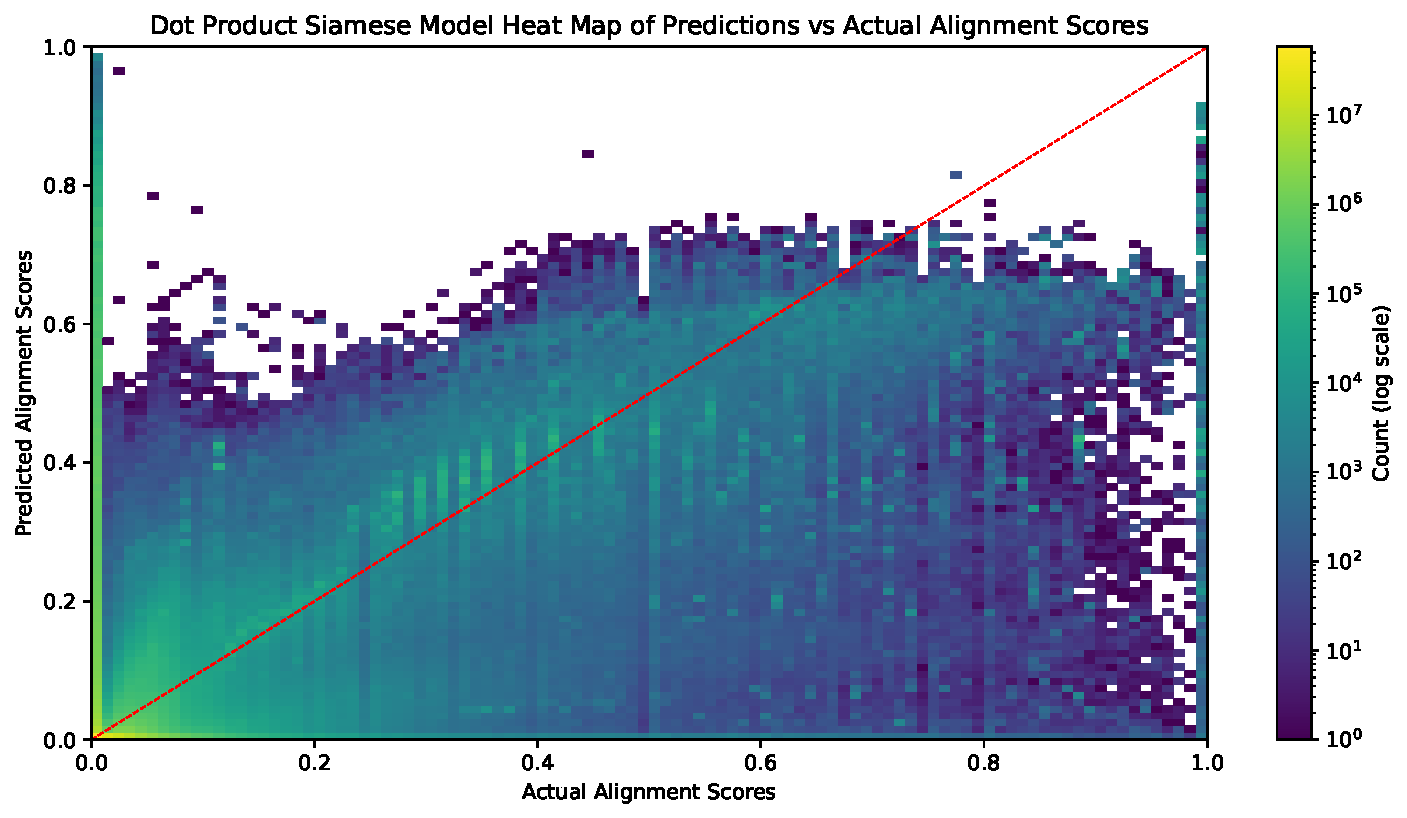
\includegraphics[scale=0.65]{Figures/Dot_Product_Siamese_Model_Heatmap.pdf}
\caption{\textbf{Frequency Heat‑map of Dot Product Siamese Model's Predictions vs. True Labels.} The colour intensity (log‑scaled count) represents the frequency in each prediction–actual score bin, and the diagonal line represents perfect agreement.} 
\label{fig:SiameseModelHeatmap}
\end{figure}

Figure \ref{fig:SiameseModelHeatmap} shows that the model achieves good prediction accuracy for alignment scores up to \textit{0.5}, with most predictions falling near the diagonal line representing perfect agreement. However, beyond this threshold, the model's predictions form a visible horizontal band plateauing at around \textit{0.7} in the predicted score range, making it less reliable for identifying highly aligned functions. This creates a ceiling effect where functions with true alignment scores between \textit{0.7-1.0} are consistently underestimated.

This limitation could be attributed to the imbalanced training data distribution, as evident from the colour intensity in the lower regions of the heat map, where the colour intensity indicates a significantly higher concentration of examples with lower alignment scores. Consequently, the model optimises its performance by learning to predict lower scores more frequently, minimising the overall loss function but compromising accuracy for high-alignment cases.

\subsection{Multi-Headed Self-Attention Model Results}
The fully trained and tuned multi-headed self-attention model demonstrated exceptional performance, achieving an MSE score of \textbf{0.00738} across the entire testing dataset and \textbf{0.00094} for the non-zero testing dataset, orders of magnitude lower than the Siamese model's MSE.


\begin{figure}[tbh!]
\centering
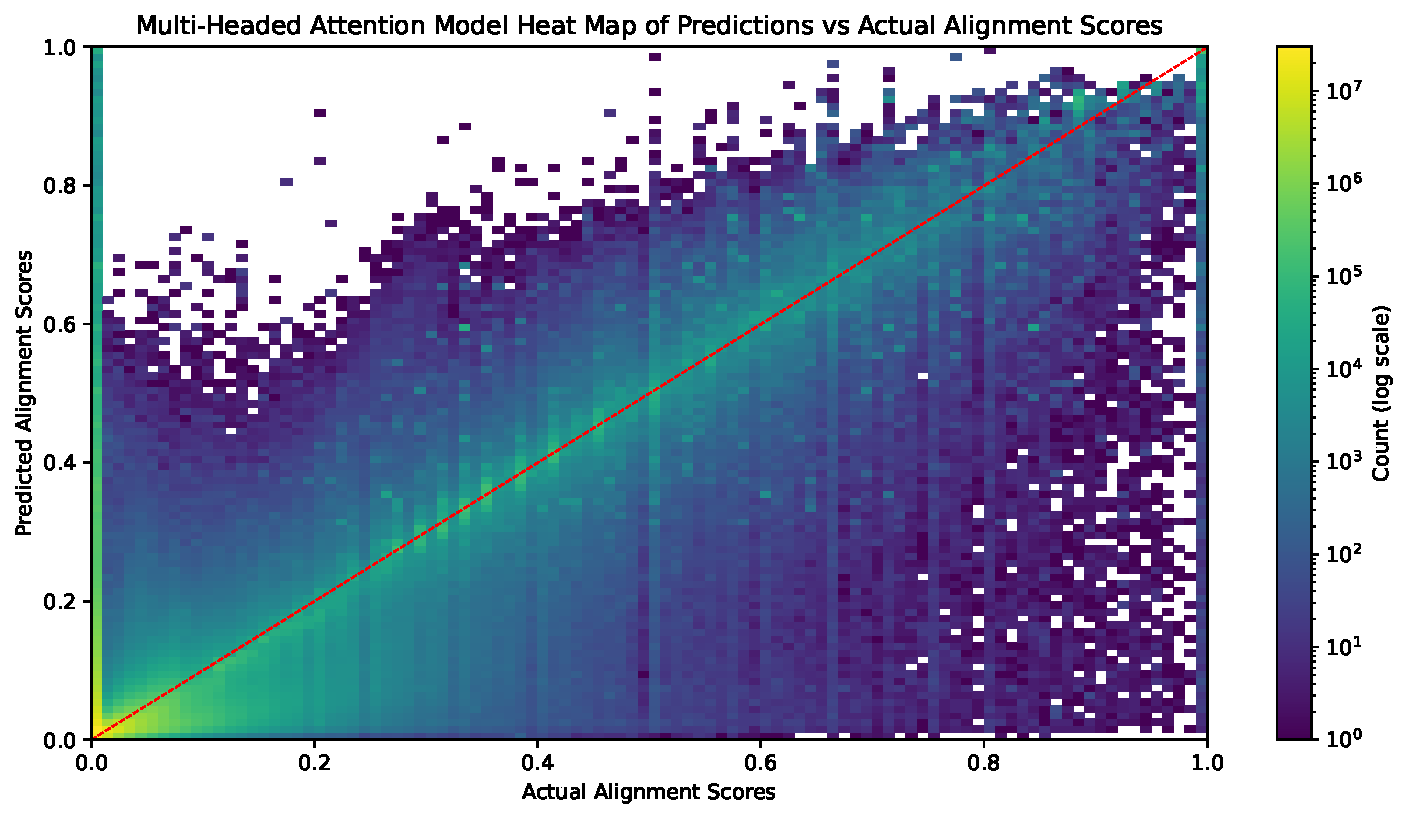
\includegraphics[scale=0.65]{Figures/Multi-Headed_Attention_Model_Heatmap.pdf}
\caption{\textbf{Frequency Heat‑map of Multi-Headed Self-Attention Model's Predictions vs. True Labels.} The colour intensity (log‑scaled count) represents the frequency in each prediction–actual score bin, and the diagonal line represents perfect agreement.} 
\label{fig:AttentionModelHeatmap}
\end{figure}

Figure \ref{fig:AttentionModelHeatmap} reveals that this model reliably predicts true alignment scores across the full spectrum of values, with most predictions closely following the diagonal line that represents perfect agreement. The heat map shows a more consistent prediction pattern along the diagonal, particularly in the 0.7-1.0 range, where the Siamese model struggled. While significantly outperforming the dot product Siamese model, this attention-based architecture still exhibits a subtle bias toward under-prediction rather than over-prediction when errors occur. However, this tendency is considerably less pronounced than in the previous model, allowing for more accurate identification of highly aligned function pairs.

\subsection{Evaluation}
Analysis of both models reveals a common pattern in figures \ref{fig:SiameseModelHeatmap} and \ref{fig:AttentionModelHeatmap}, where samples with a true score of 0 are frequently misclassified. This observation, however, should be contextualised by the significant class imbalance in the dataset, with zero-alignment samples vastly outnumbering others, as indicated by the bright yellow/green regions at the origin of both heat maps. Notably, for both models, prediction errors decrease as the predicted values move away from 0, indicating robust capabilities even with imbalanced training data.

When directly comparing performance, the self-attention model demonstrates substantially superior prediction accuracy across the entire alignment score range, particularly for the higher alignment scores where the Siamese model's plateauing effect limits its utility. The visual difference between the two heat maps is striking. The attention model shows a much more defined diagonal pattern throughout the entire range, especially above \textit{0.7}. The practical implication of implementing the Siamese model in a production environment may result in missed opportunities for merging highly-aligned function pairs due to systematic under-prediction, potentially reducing the system's overall effectiveness. Conversely, the attention model's more balanced error distribution makes it a more reliable choice for accurately identifying candidates for function merging across the full spectrum of alignment scores.

The comparative analysis reveals that the attention architecture is more forgiving towards data imbalance, maintaining high performance even with minimal pre-processing techniques. On the other hand, the Siamese architecture exhibits clear limitations when trained on skewed distributions, suggesting that it would benefit from more sophisticated pre-processing approaches. This fundamental difference in how each architecture handles class imbalance represents an important consideration for deployment scenarios where balanced training data cannot be guaranteed.

\section{Quality of Merging Predictions} \label{Eval:MergeQuality}
Next, we evaluate how well the predicted alignment scores serve as indicators for profitable function merging compared to F3M. Although the ML models may accurately estimate alignment values, those predictions may not translate into correct merge decisions. To assess and compare the quality of the merging decisions between F3M and the ML approach, function merging was applied on \textit{SPEC CPU 2006} and \textit{SPEC CPU 2017} benchmarks, using the model to predict scores for previously seen function pairs.

The function selection process for the predictive approach mirrors F3M's search method for the optimal merge candidate for each function (\ref{F3M}). Instead of using MinHash and LSH, it finds the optimal candidate by selecting the function with the highest alignment score. If this score exceeds a pre-determined threshold, 0.4, 0.5 and 0.6 are tested, the two functions are considered for merging. This thresholding strategy aims to reduce the compile time by eliminating low-potential merging attempts that would likely prove unprofitable. The merging process yields two outcomes, whether it is possible to merge the functions (\textbf{validity}) and, if valid, whether the merged function is predicted to be \textbf{profitable} in terms of binary code size reduction by using LLVM's internal cost model to estimate the function sizes.

This evaluation employs two metrics in combination to quantify the quality of the predictions, the number of total merges made and the number of profitable merges, to calculate the percentage of profitable merge attempts (\ref{METRIC:ProfitablePercentage}). These metrics will be plotted for each benchmark to visualise their merging quality.

\subsection{Number of Attempted Merges}
Figure \ref{fig:AttemptedMerges} collectively shows the number of attempted function merges for F3M, dot product model prediction approach and the attention model prediction approach across all prediction threshold values.

\begin{figure}[p!]
    \centering
    \begin{subfigure}{\textwidth}
        \centering
        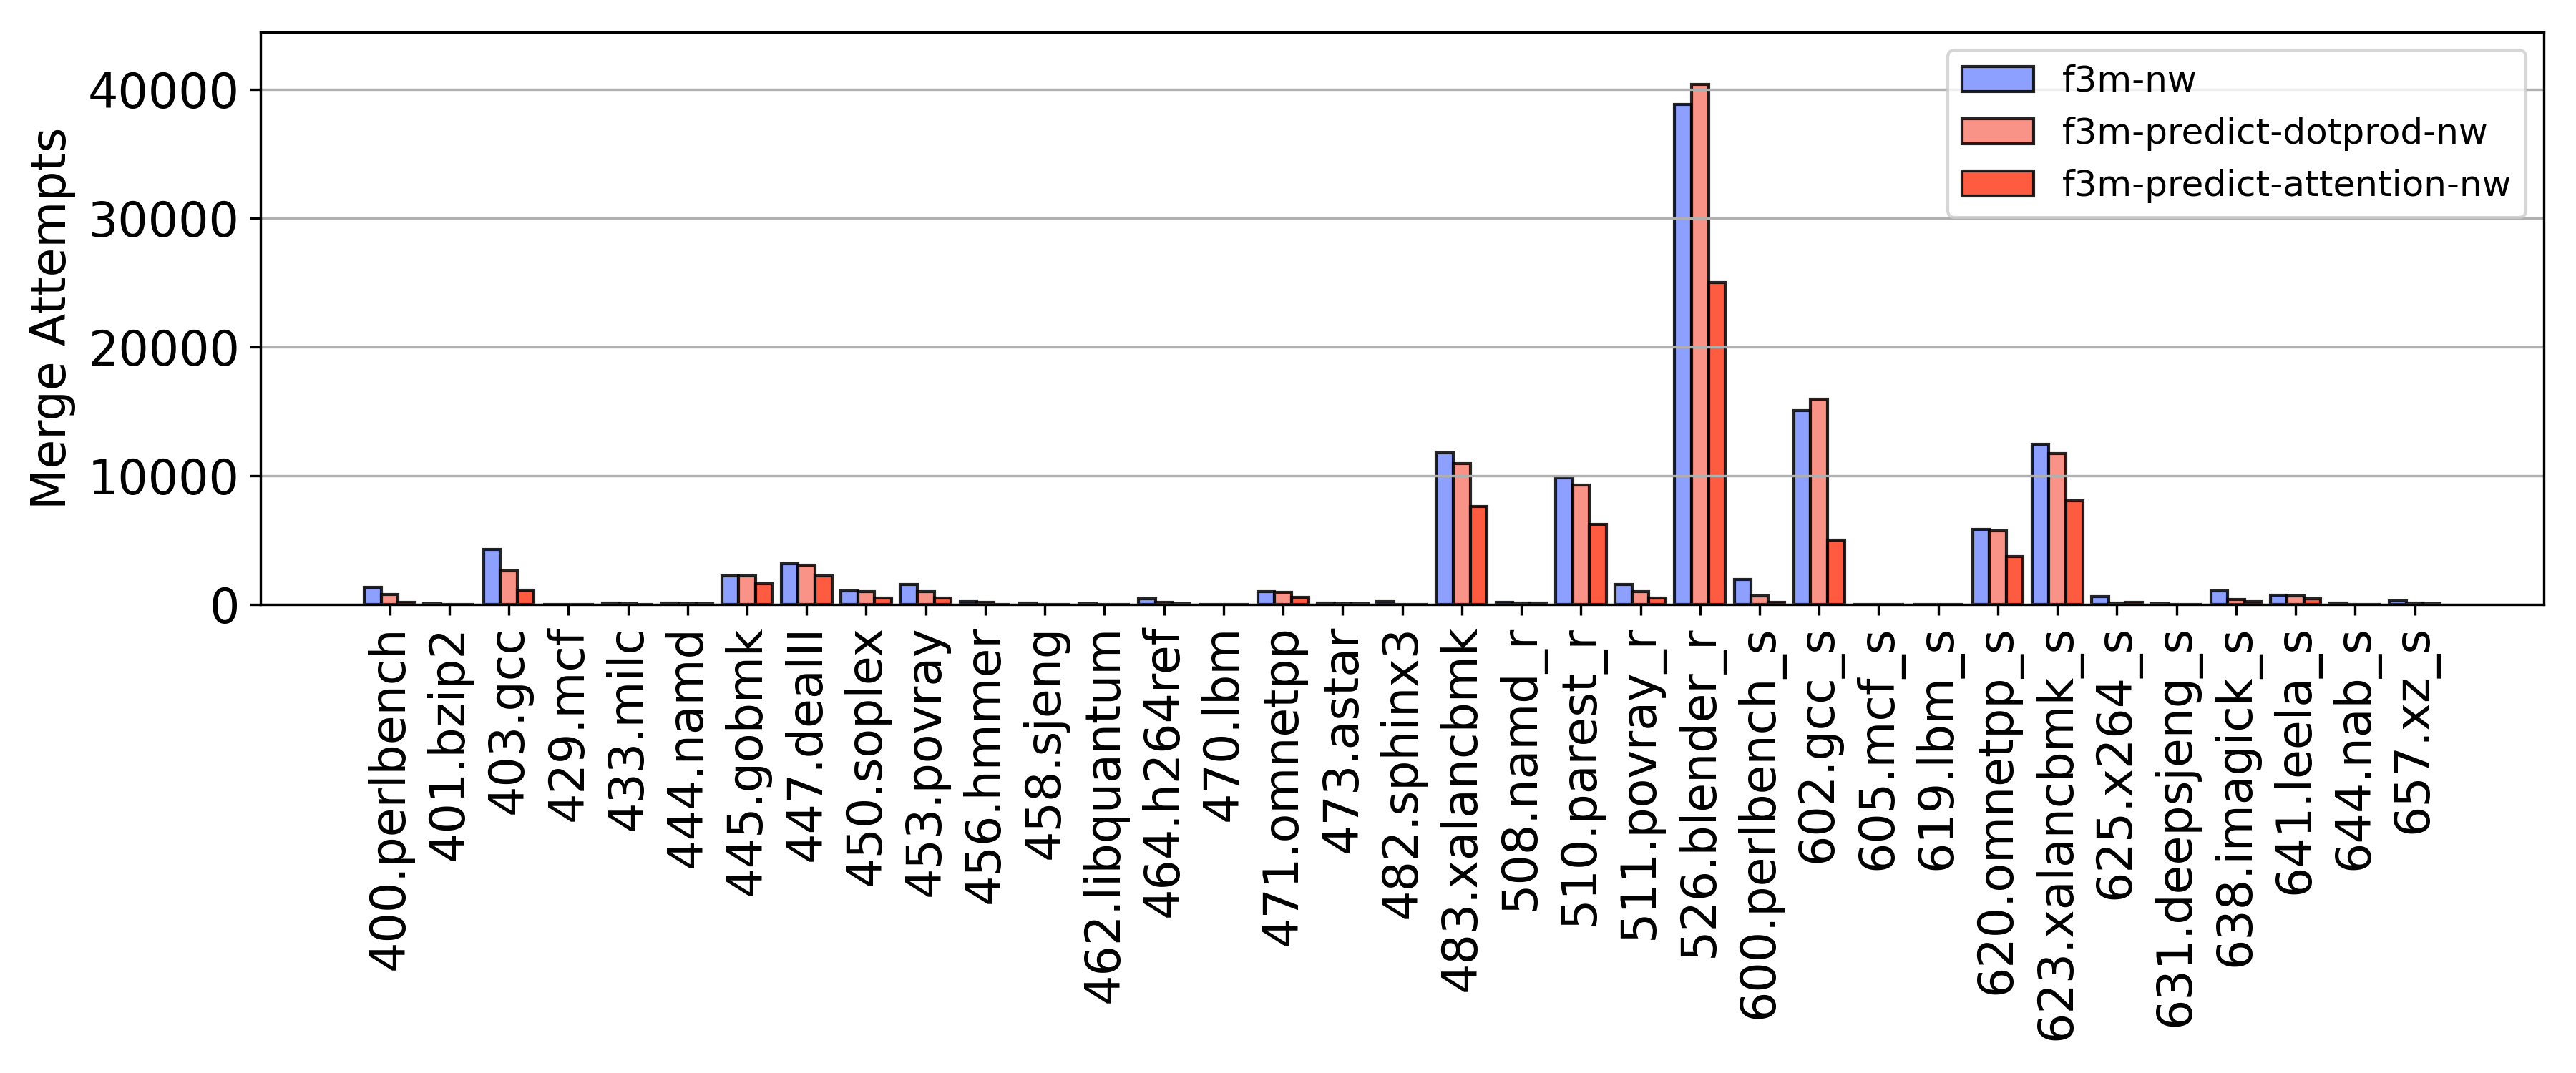
\includegraphics[scale=0.47]{Figures/Valid_Merging_Predictions/0.4_MergeAttempts.png}
        \caption{\textbf{Number of Attempted Merges (\textbf{0.4} Threshold)}} 
        \label{fig:0.4AttemptedMerges}
    \end{subfigure}
    \begin{subfigure}{\textwidth}
        \centering
        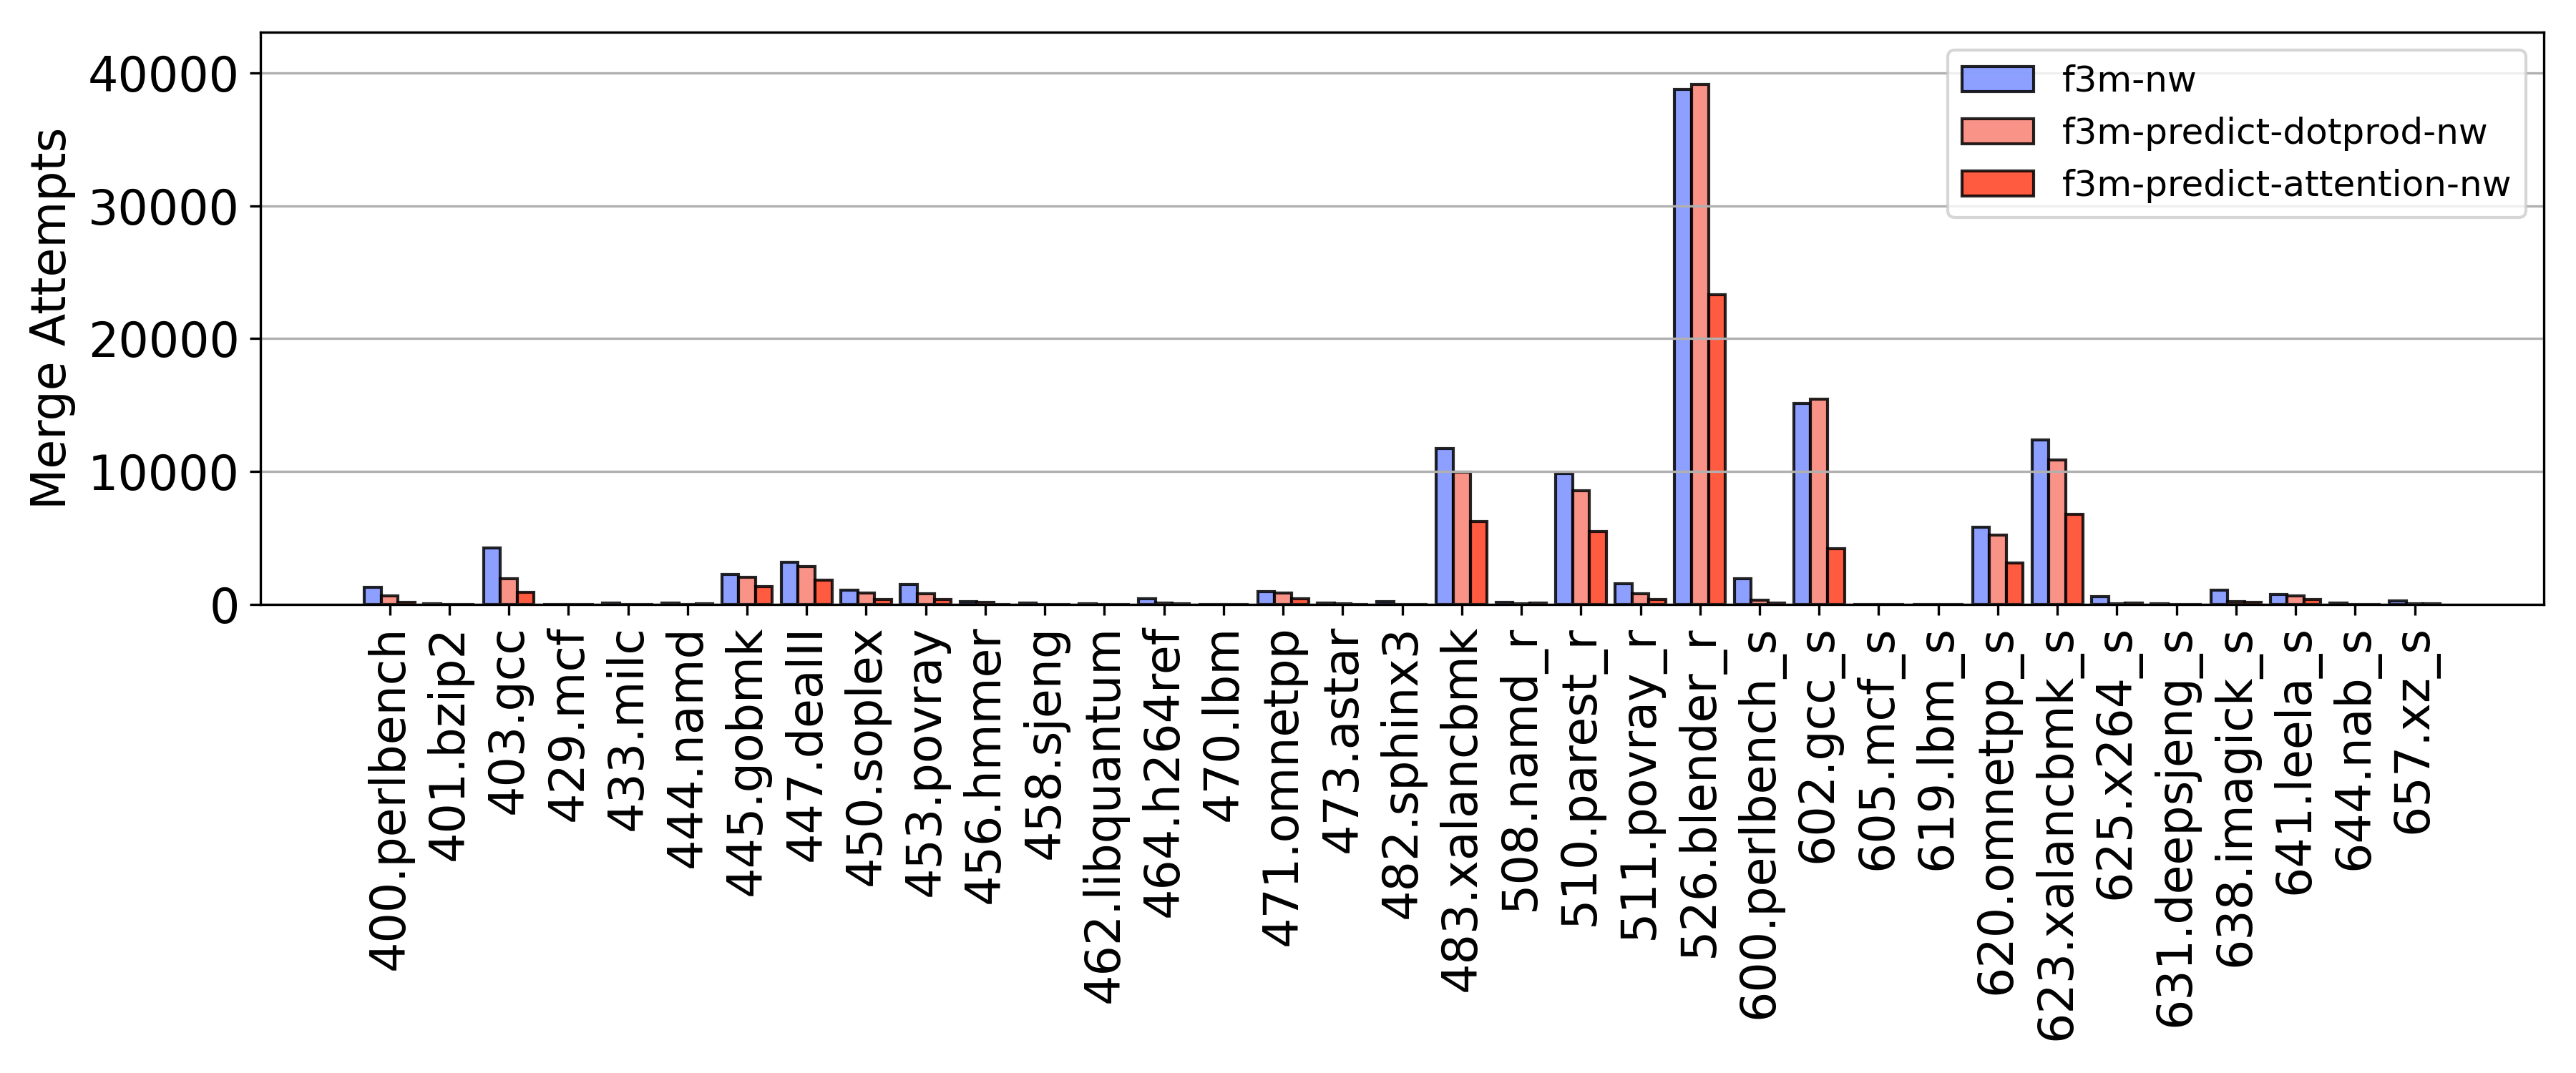
\includegraphics[scale=0.47]{Figures/Valid_Merging_Predictions/0.5_MergeAttempts.png}
        \caption{\textbf{Number of Attempted Merges (\textbf{0.5} Threshold)}} 
        \label{fig:0.5AttemptedMerges}
    \end{subfigure}
    \begin{subfigure}{\textwidth}
    \centering
        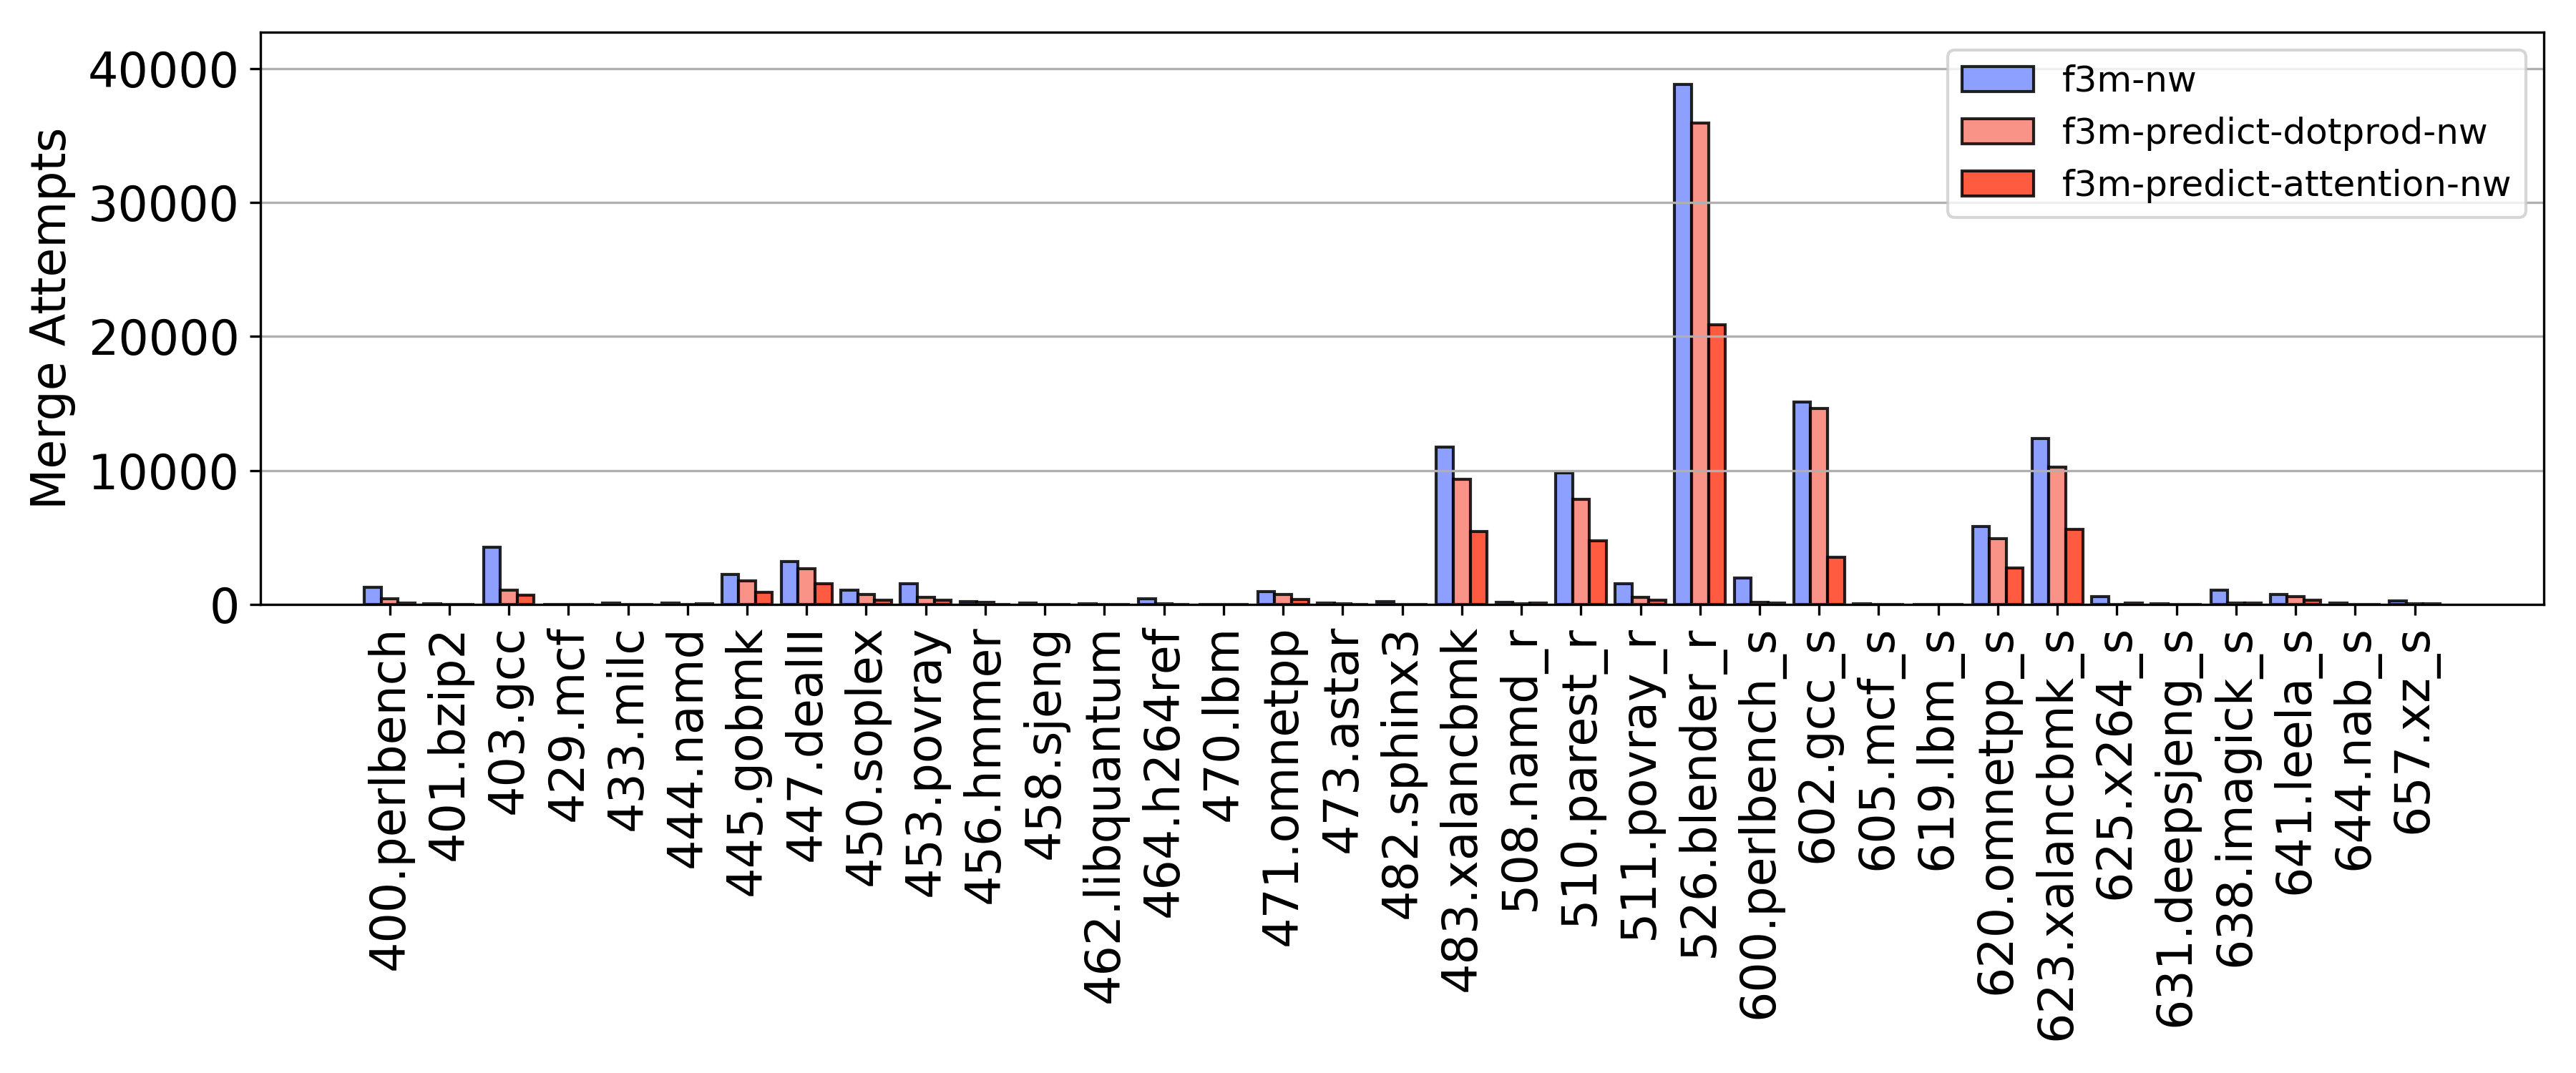
\includegraphics[scale=0.47]{Figures/Valid_Merging_Predictions/0.6_MergeAttempts.png}
        \caption{\textbf{Number of Attempted Merges (\textbf{0.6} Threshold)}} 
        \label{fig:0.6AttemptedMerges}
    \end{subfigure}

    \caption{\textbf{Number of Attempted Merges} for each threshold.} 
    \label{fig:AttemptedMerges}
\end{figure}

The benchmark \textit{526.blender\_r} exhibits the most merging attempts, more than double that of the next highest benchmark, while \textit{429.mcf} and \textit{605.mcf\_s} have the least attempted merges. This disparity indicates that blender contains many function candidates for function merging operations, while mcf offers a limited number of options, restricting the potential for merging due to the lack of available pairs.

As the threshold increases, both predictive models demonstrate an inverse correlation with the number of merge attempts as expected. This effect is particularly pronounced in the dot product model, which initially attempts more merges than F3M in some cases at a threshold of 0.4, matches F3M generally at 0.5, and finally, fewer merges at a threshold of 0.6. In contrast, the attention model consistently predicts significantly fewer suitable functions to merge than the other two implementations across the whole benchmark suite, with some cases such as \textit{602.gcc\_s} showing more than 50\% fewer attempts.



\subsection{Profitability of Attempted Merges}
Finally, figure \ref{fig:ProfitableMerges} graphs the percentage of merges that produced a profitable merged function across all 35 benchmarks at three similarity thresholds. Profitability is determined when the estimated size of the newly merged function is smaller than the sum of the estimated sizes of the original function pair.

\begin{figure}[p!]
    \centering
    \begin{subfigure}{\textwidth}
        \centering
        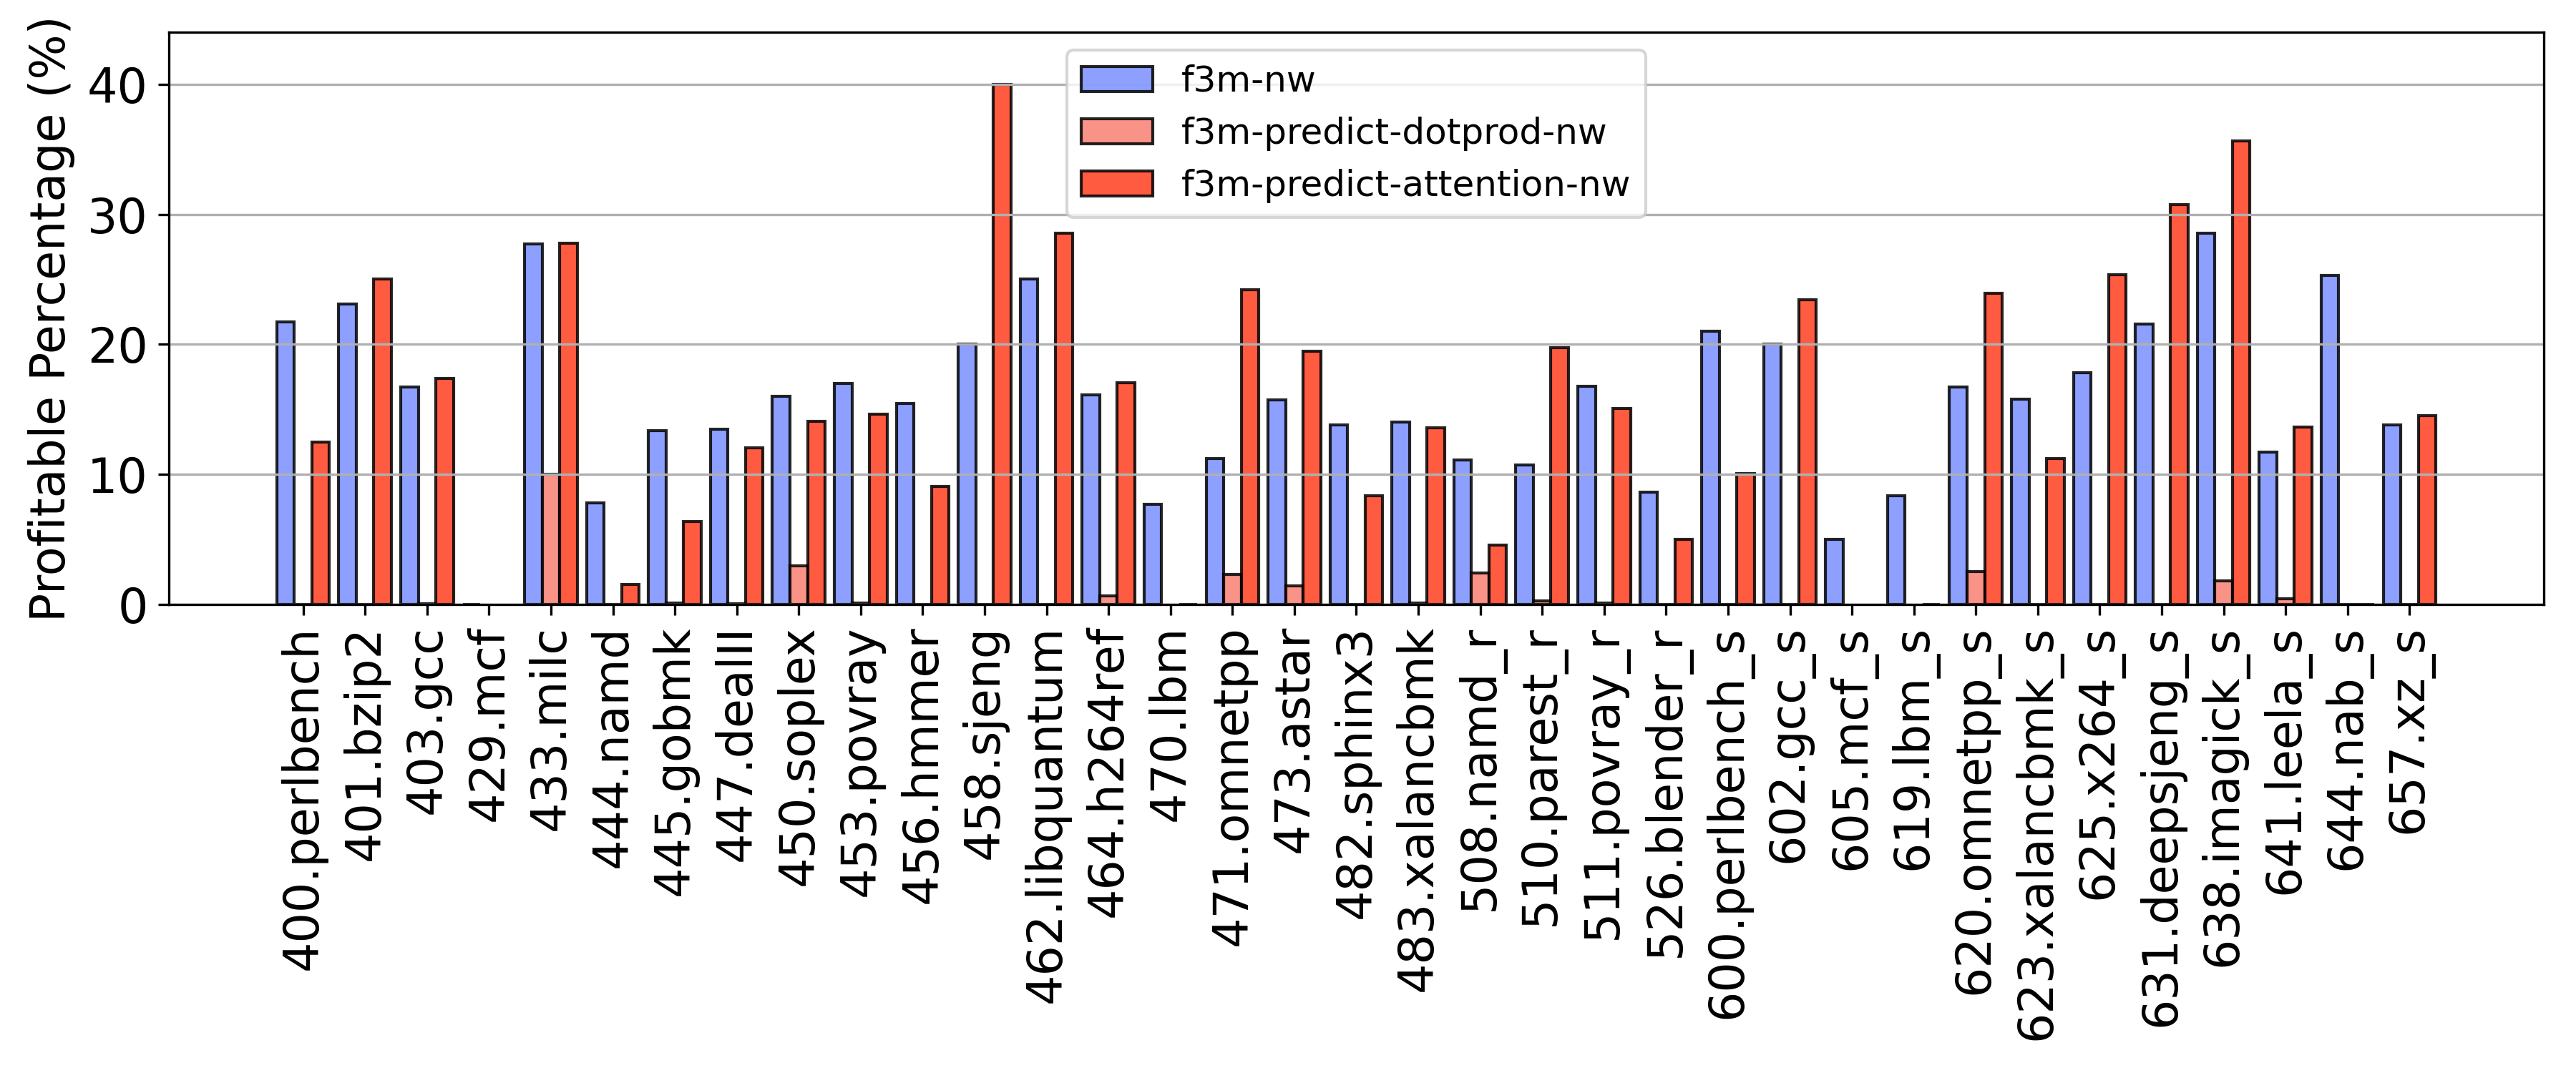
\includegraphics[scale=0.47]{Figures/Valid_Merging_Predictions/0.4_ProfitablePercentage.png}
        \caption{\textbf{Profitable Merge Attempts (\textbf{0.4} Threshold)}} 
        \label{fig:0.4ProfitableMerges}
    \end{subfigure}
    \begin{subfigure}{\textwidth}
        \centering
        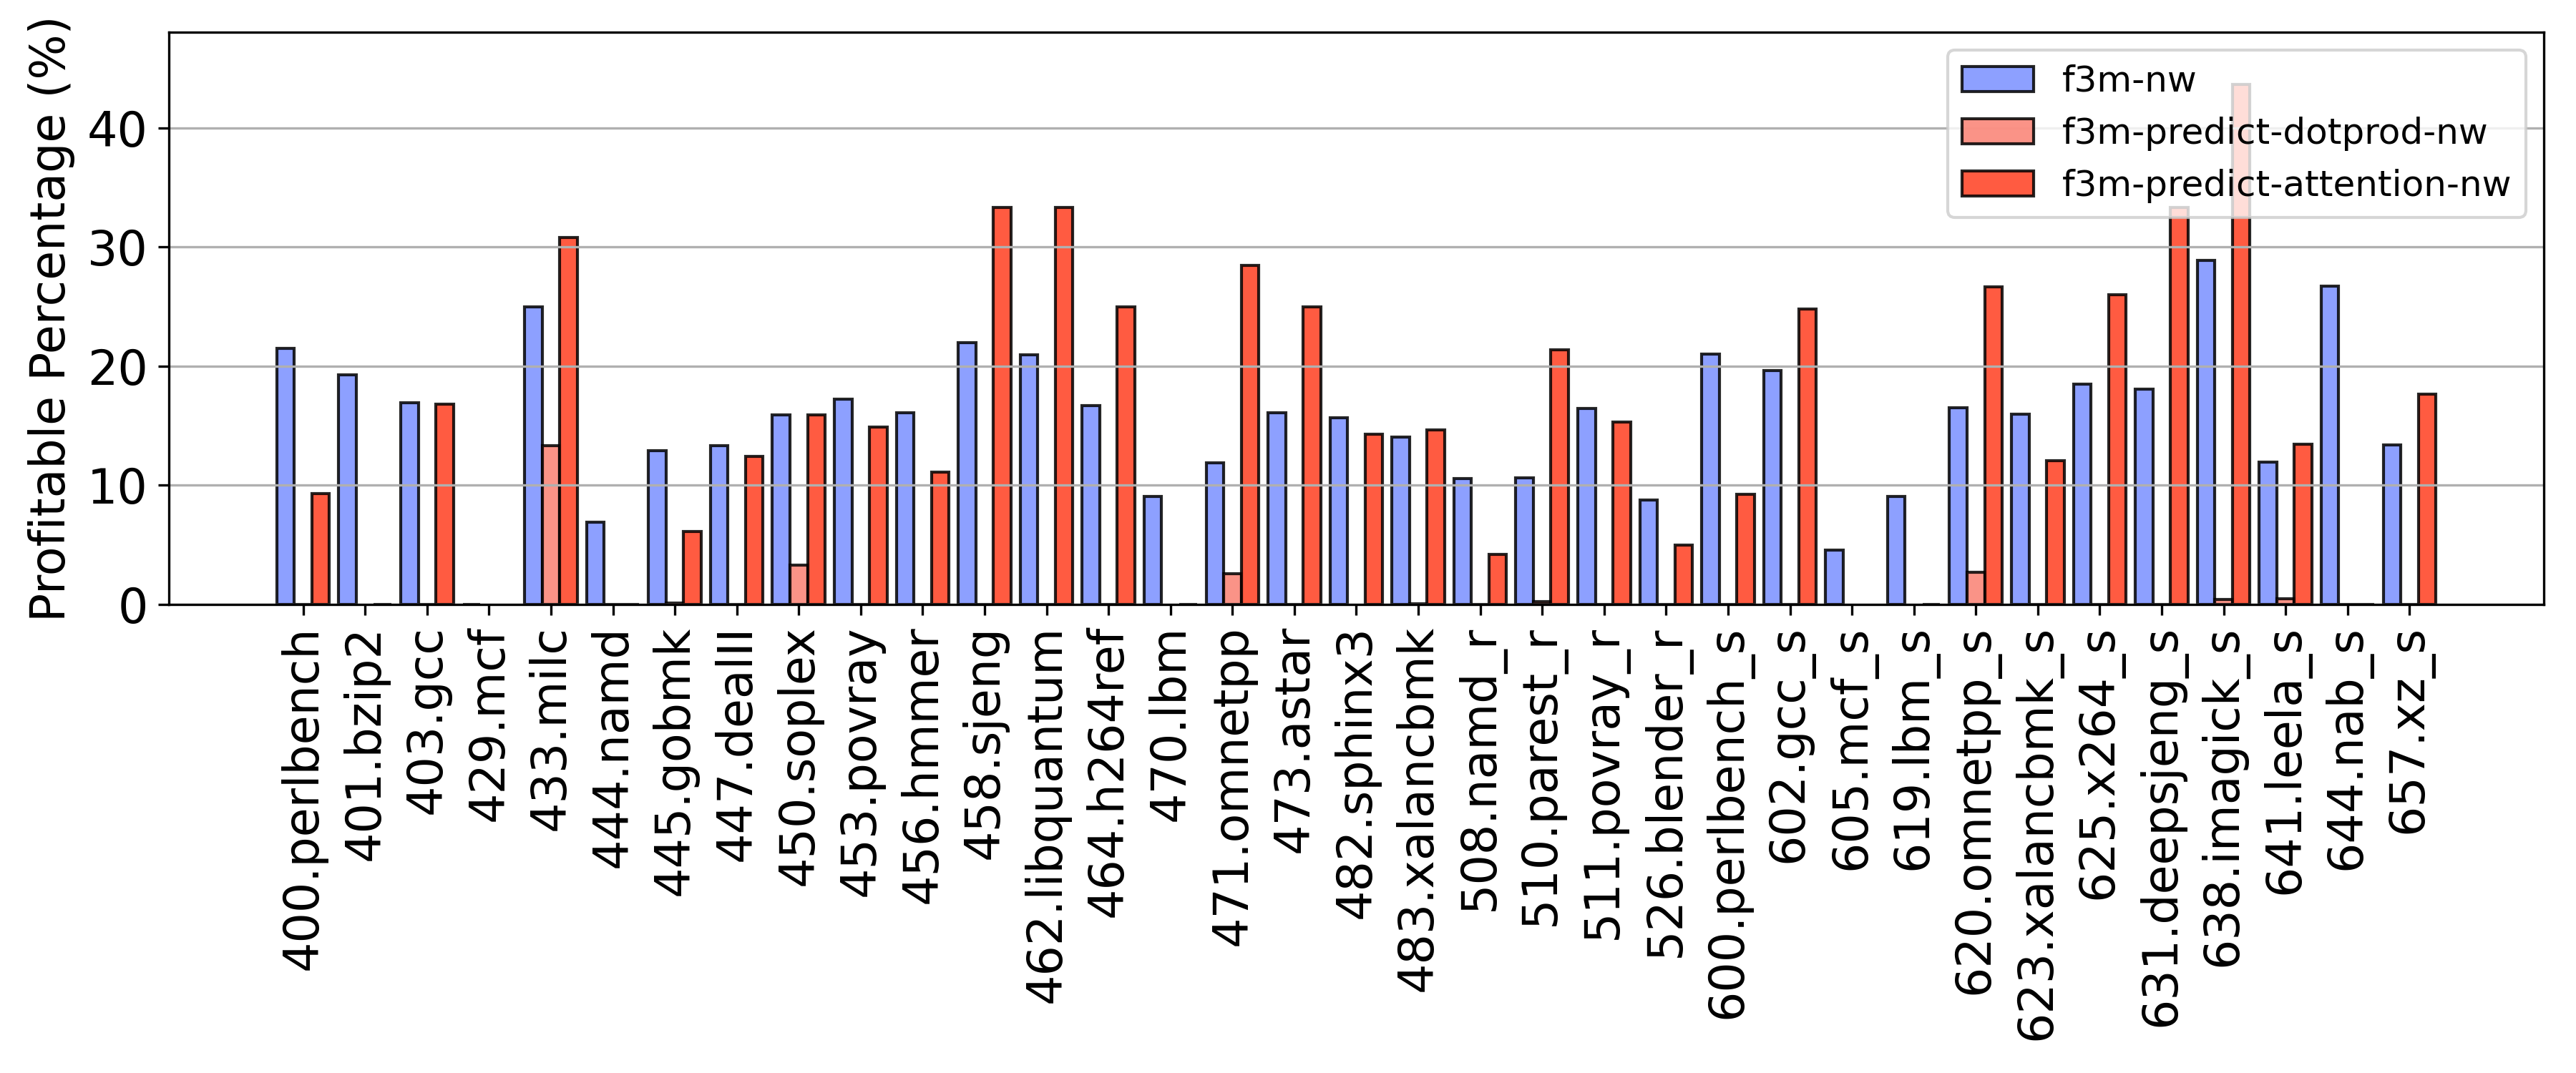
\includegraphics[scale=0.47]{Figures/Valid_Merging_Predictions/0.5_ProfitablePercentage.png}
        \caption{\textbf{Profitable Merge Attempts (\textbf{0.5} Threshold)}} 
        \label{fig:0.5ProfitableMerges}
    \end{subfigure}
    \begin{subfigure}{\textwidth}
    \centering
        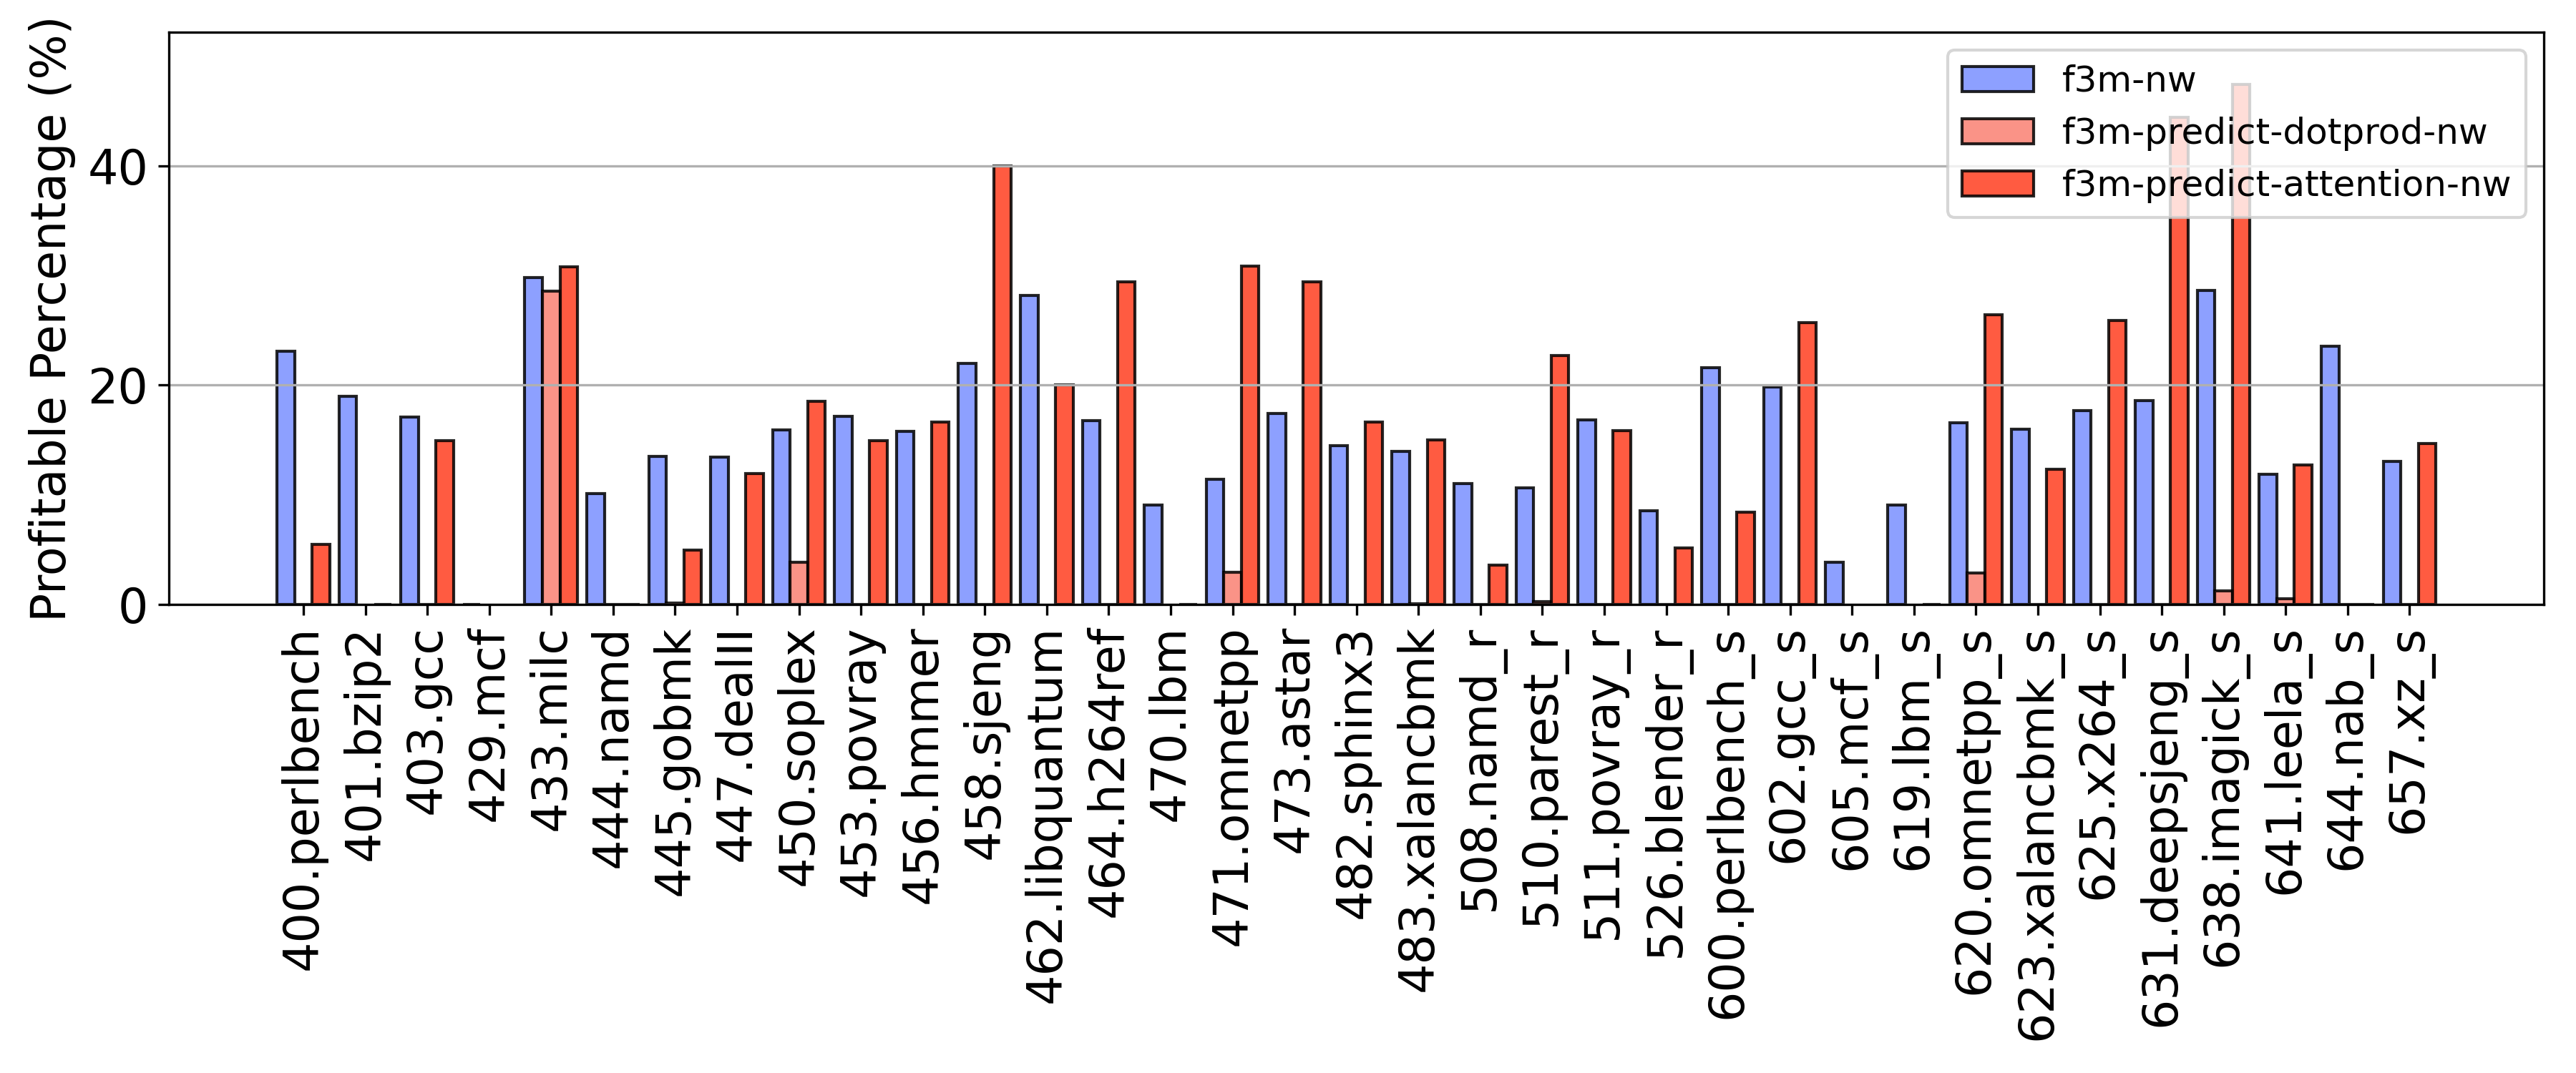
\includegraphics[scale=0.47]{Figures/Valid_Merging_Predictions/0.6_ProfitablePercentage.png}
        \caption{\textbf{Profitable Merge Attempts (\textbf{0.6} Threshold)}} 
        \label{fig:0.6ProfitableMerges}
    \end{subfigure}

    \caption{\textbf{Percentage of merge attempts that are profitable} for each threshold. This graph illustrates the proportion of merge attempts that result in smaller function size calculated using equation \ref{METRIC:ProfitablePercentage}.} 
    \label{fig:ProfitableMerges}
\end{figure}



Overall, the dot‐product approach struggles to identify merge-able pairs regardless of threshold. It rarely breaks the 2.5\% mark, achieving its best result of 29\% on the \textit{433.milc} benchmark at the 0.6 threshold. On the other hand, the attention-based approach matches or exceeds F3M on 18 out of 35 benchmarks (just over half), peaking at a 47.5\% profitable‐merge rate on \textit{638.imagick\_s} when thresholded at 0.6.

\subsection{Evaluation}
The Dot Product Model demonstrates significant limitations as a heuristic for function merging. Despite proposing similar merges to F3M, its precision remains unacceptably low, topping out at 29\% valid merges on the \textit{433.milc} benchmark at a 0.6 threshold. This indicates that over 70\% of its attempted merges are unprofitable and cannot identify profitable function pairs, representing substantial wasted computational effort during compilation, rendering it an unreliable indicator of merging performance.

The attention model presents a more conservative approach than F3M, generating significantly fewer merge attempts than F3M, sometimes less than half as many. This reduction raises two possible interpretations, either the model fails to identify viable merging opportunities that F3M captures or achieves superior global optimisation by prioritising the most beneficial merges first, leaving fewer similar functions available for subsequence merges. When profitability is considered, the attention model maintains consistent performance across all tested thresholds, showing promising prediction quality.

The evidence indicates that the Attention Model substantially outperforms the Dot Product Model as a function merging heuristic. Despite its high proposal volume, the Dot Product approach suffers from a poor, unprofitable merge rate. In contrast, the Attention Model delivers noticeably better profitability across all thresholds. Further evaluation is needed to determine whether the Attention Model's reduced attempt count represents optimality or overlooks merges.

% While both prediction models demonstrate superior precision in selecting profitable merging candidates when they succeed in finding valid pairs, the attention model's combination of reasonable valid merge counts and high profitability makes it the more promising approach for real-world compiler optimisation scenarios.


% =================================================
% \newpage
% This evaluation employs three metrics in combination to quantify the quality of the predictions: the number of total merges made, the number of valid merges and the number of profitable merges.

% For each function, the system identifies another function with the highest alignment score as a potential merging candidate. If this score exceeds a pre-determined threshold, the two functions are considered for merging. This thresholding strategy aims to reduce the compile time by eliminating low-potential merging attempts that would likely prove unprofitable. The merging process yields two outcomes, whether it is possible to merge the functions (\textbf{validity}) and if valid, whether the merged function is \textbf{profitable}. 

% The evaluation uses three plots to visualise the quality of the predictions:
% \begin{itemize}
%     \item The total number of attempted merges
%     \item The percentage of merges that are valid
%     \item The percentage of valid merges that are profitable
% \end{itemize}
% These percentages are calculated using equations \ref{METRIC:ValidPercentage} and \ref{METRIC:ValidProfitablePercentage} respectively. The evaluation assesses the quality of the predictions across three thresholds: 0.4, 0.5, and 0.6. 

% \begin{equation} \label{METRIC:ValidPercentage}
%     Valid\ Percentage(\%) =\frac{No.\ of\ Valid\ Merges}{Total\ No.\ of\ Attempted\ Merges}
% \end{equation}

% \begin{equation} \label{METRIC:ValidProfitablePercentage}
%     Valid\ Profitable\ Percentage (\%)=\frac{No.\ of\ Profitable\ Merges}{No.\ of\ Valid\ Merges}
% \end{equation}


% \subsection{Number of Attempted Merges}
% Figure \ref{fig:AttemptedMerges} collectively show the number of attempted function merges for F3M, dot product model prediction approach and the attention model prediction approach across all prediction threshold values.

% \begin{figure}[tbh!]
%     \centering
%     \begin{subfigure}{\textwidth}
%         \centering
%         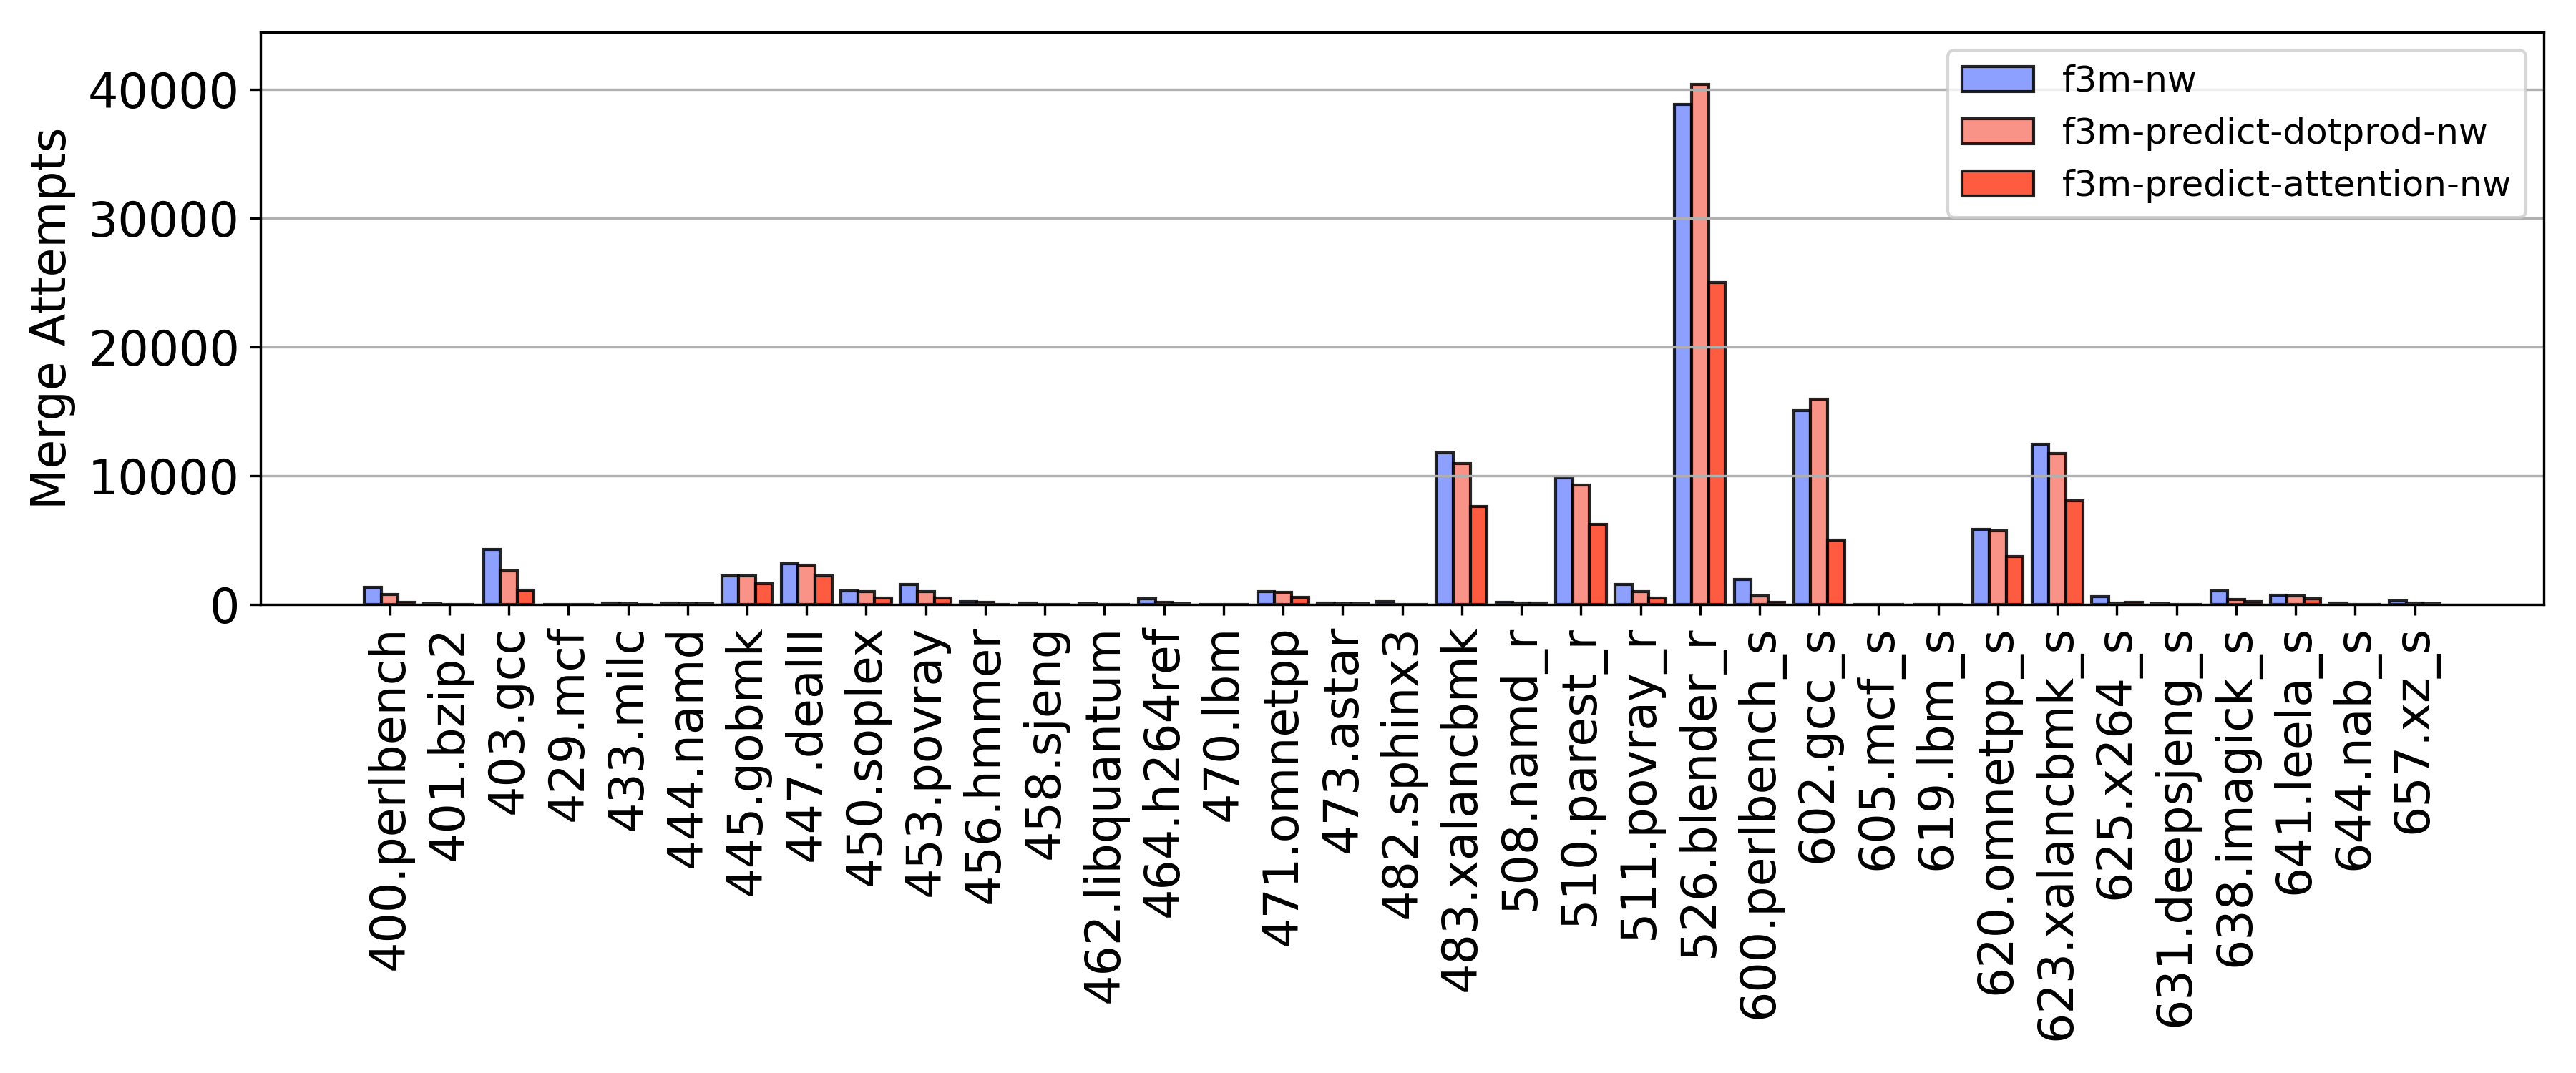
\includegraphics[scale=0.47]{Figures/Valid_Merging_Predictions/0.4_MergeAttempts.png}
%         \caption{\textbf{Number of Attempted Merges (\textbf{0.4} Threshold)}} 
%         \label{fig:0.4AttemptedMerges}
%     \end{subfigure}
%     \begin{subfigure}{\textwidth}
%         \centering
%         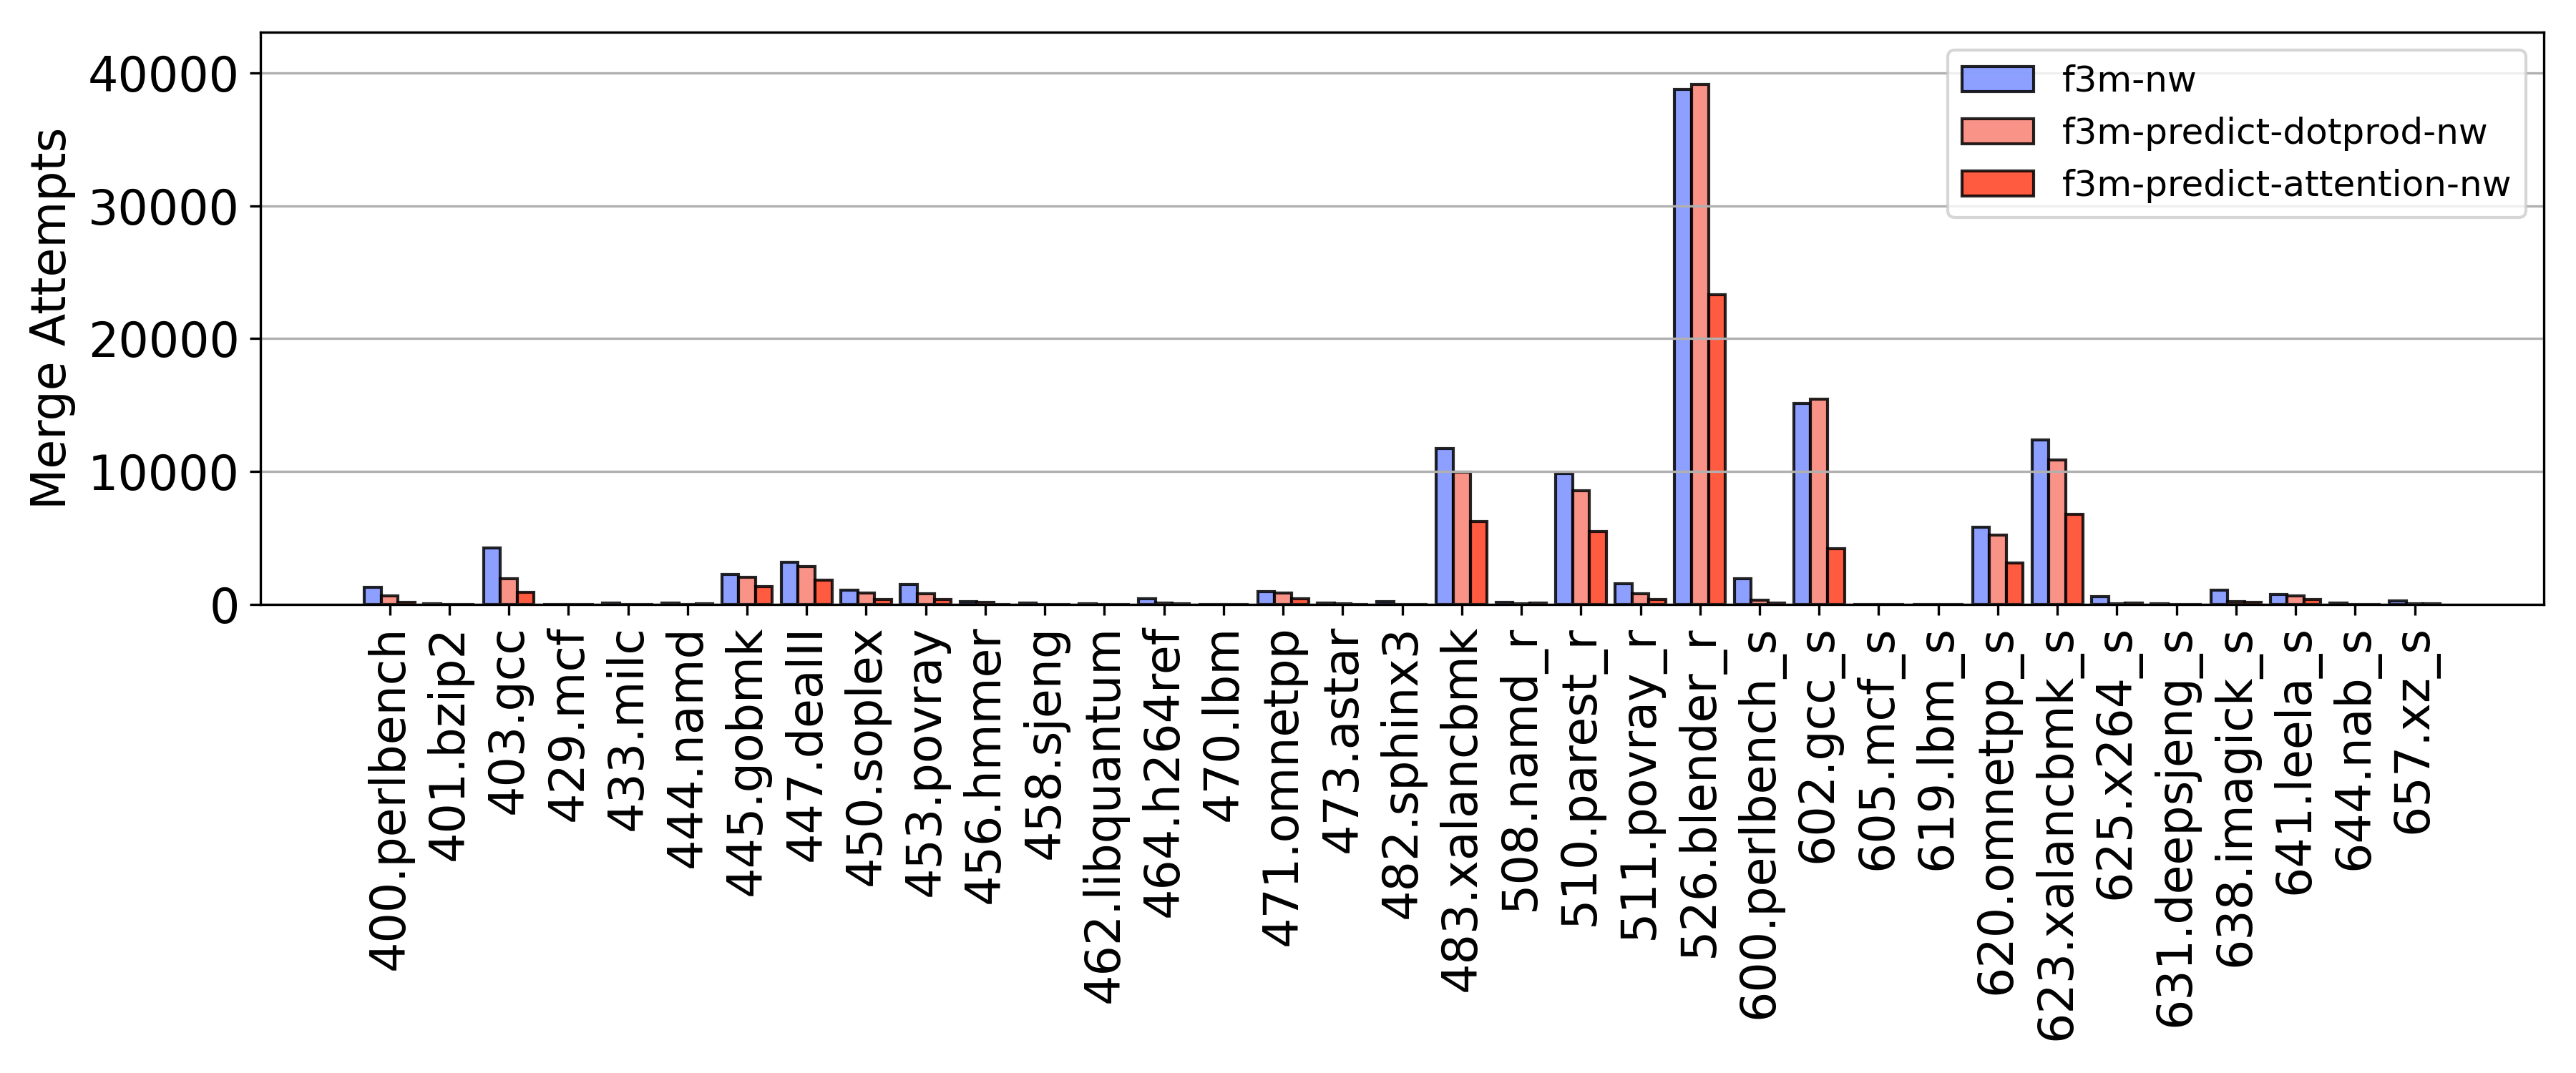
\includegraphics[scale=0.47]{Figures/Valid_Merging_Predictions/0.5_MergeAttempts.png}
%         \caption{\textbf{Number of Attempted Merges (\textbf{0.5} Threshold)}} 
%         \label{fig:0.5AttemptedMerges}
%     \end{subfigure}
%     \begin{subfigure}{\textwidth}
%     \centering
%         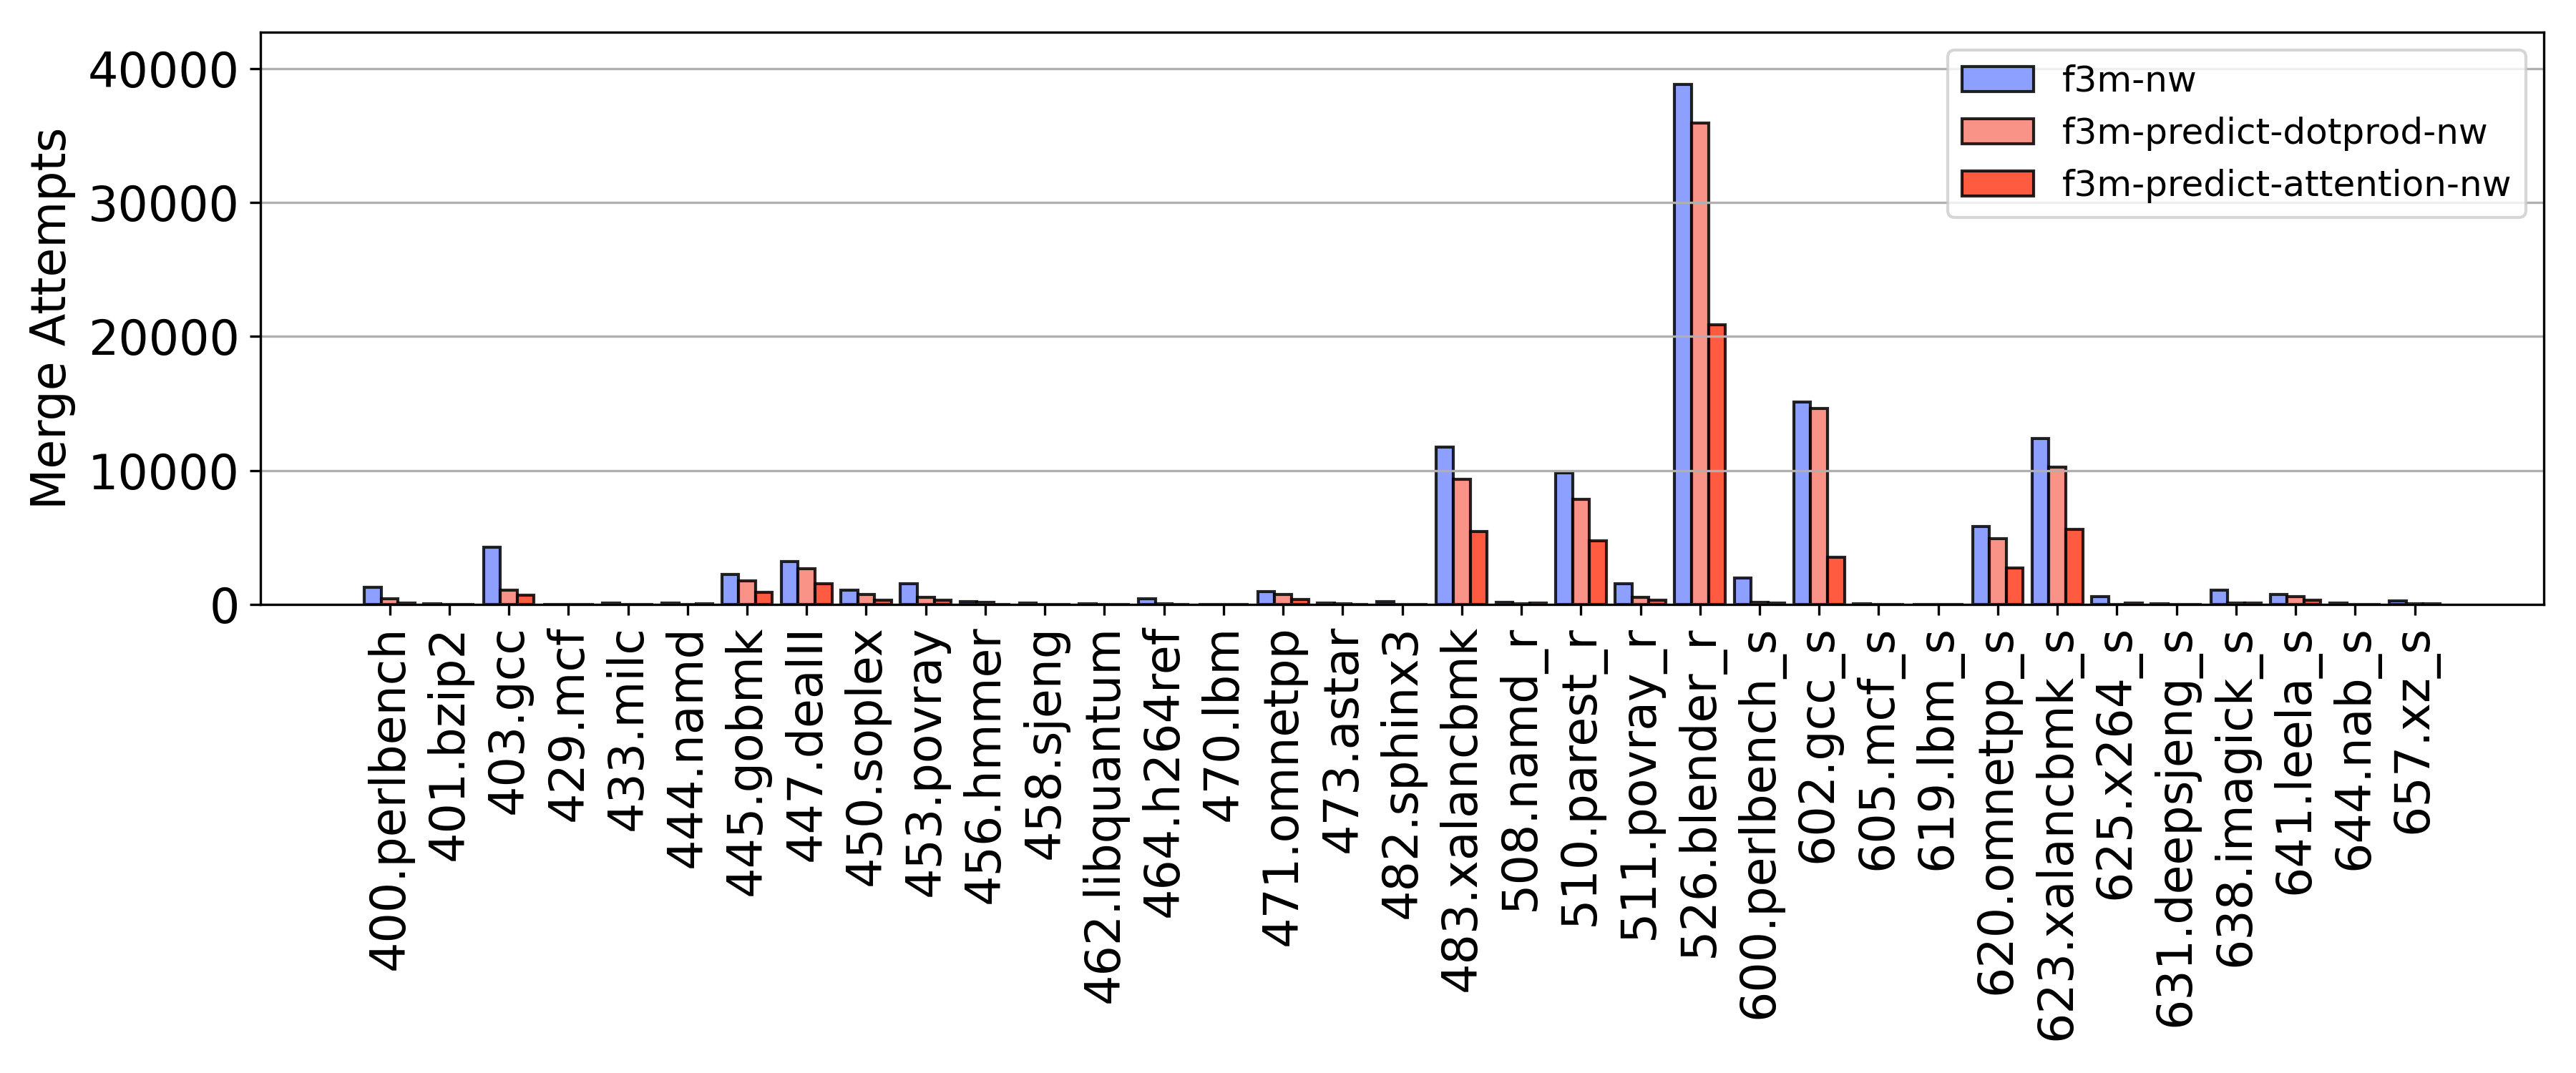
\includegraphics[scale=0.47]{Figures/Valid_Merging_Predictions/0.6_MergeAttempts.png}
%         \caption{\textbf{Number of Attempted Merges (\textbf{0.6} Threshold)}} 
%         \label{fig:0.6AttemptedMerges}
%     \end{subfigure}

%     \caption{\textbf{Number of Attempted Merges} for each threshold.} 
%     \label{fig:AttemptedMerges}
% \end{figure}

% The benchmark \textit{526.blender\_r} exhibits the most merging attempts, more than double that of the next highest benchmark, while \textit{429.mcf} and \textit{605.mcf\_s} have the least amount of attempted merges. This disparity indicates that blender contains a lot of function candidates for function merging operations, while mcf offers a limited number of options, restricting the potential for merging due to the lack of available pairs.

% As the threshold increases, both predictive models demonstrate an inverse correlation with the number of merge attempts as expected. This effect is particularly pronounced in the dot product model, which initially attempts more merges than F3M in some cases at a threshold of 0.4, matches F3M generally at 0.5, and finally predicts fewer function merges at a threshold of 0.6. In contrast, the attention model consistently predicts significantly fewer suitable functions to merge than the other two implementations across the whole benchmark suite, with some cases such as \textit{602.gcc\_s} showing more than 50\% fewer attempts.



% \subsection{Validity of Merging Attempts}
% Figure \ref{fig:Valid} plot the ratio of the attempted merges that were able to produce a merged function (validity) for each prediction threshold. This validity metric allows us to normalise the data against the varying attempted merges and compare performance across the implementations.

% \begin{figure}[tbh!]
%     \centering
%     \begin{subfigure}{\textwidth}
%         \centering
%         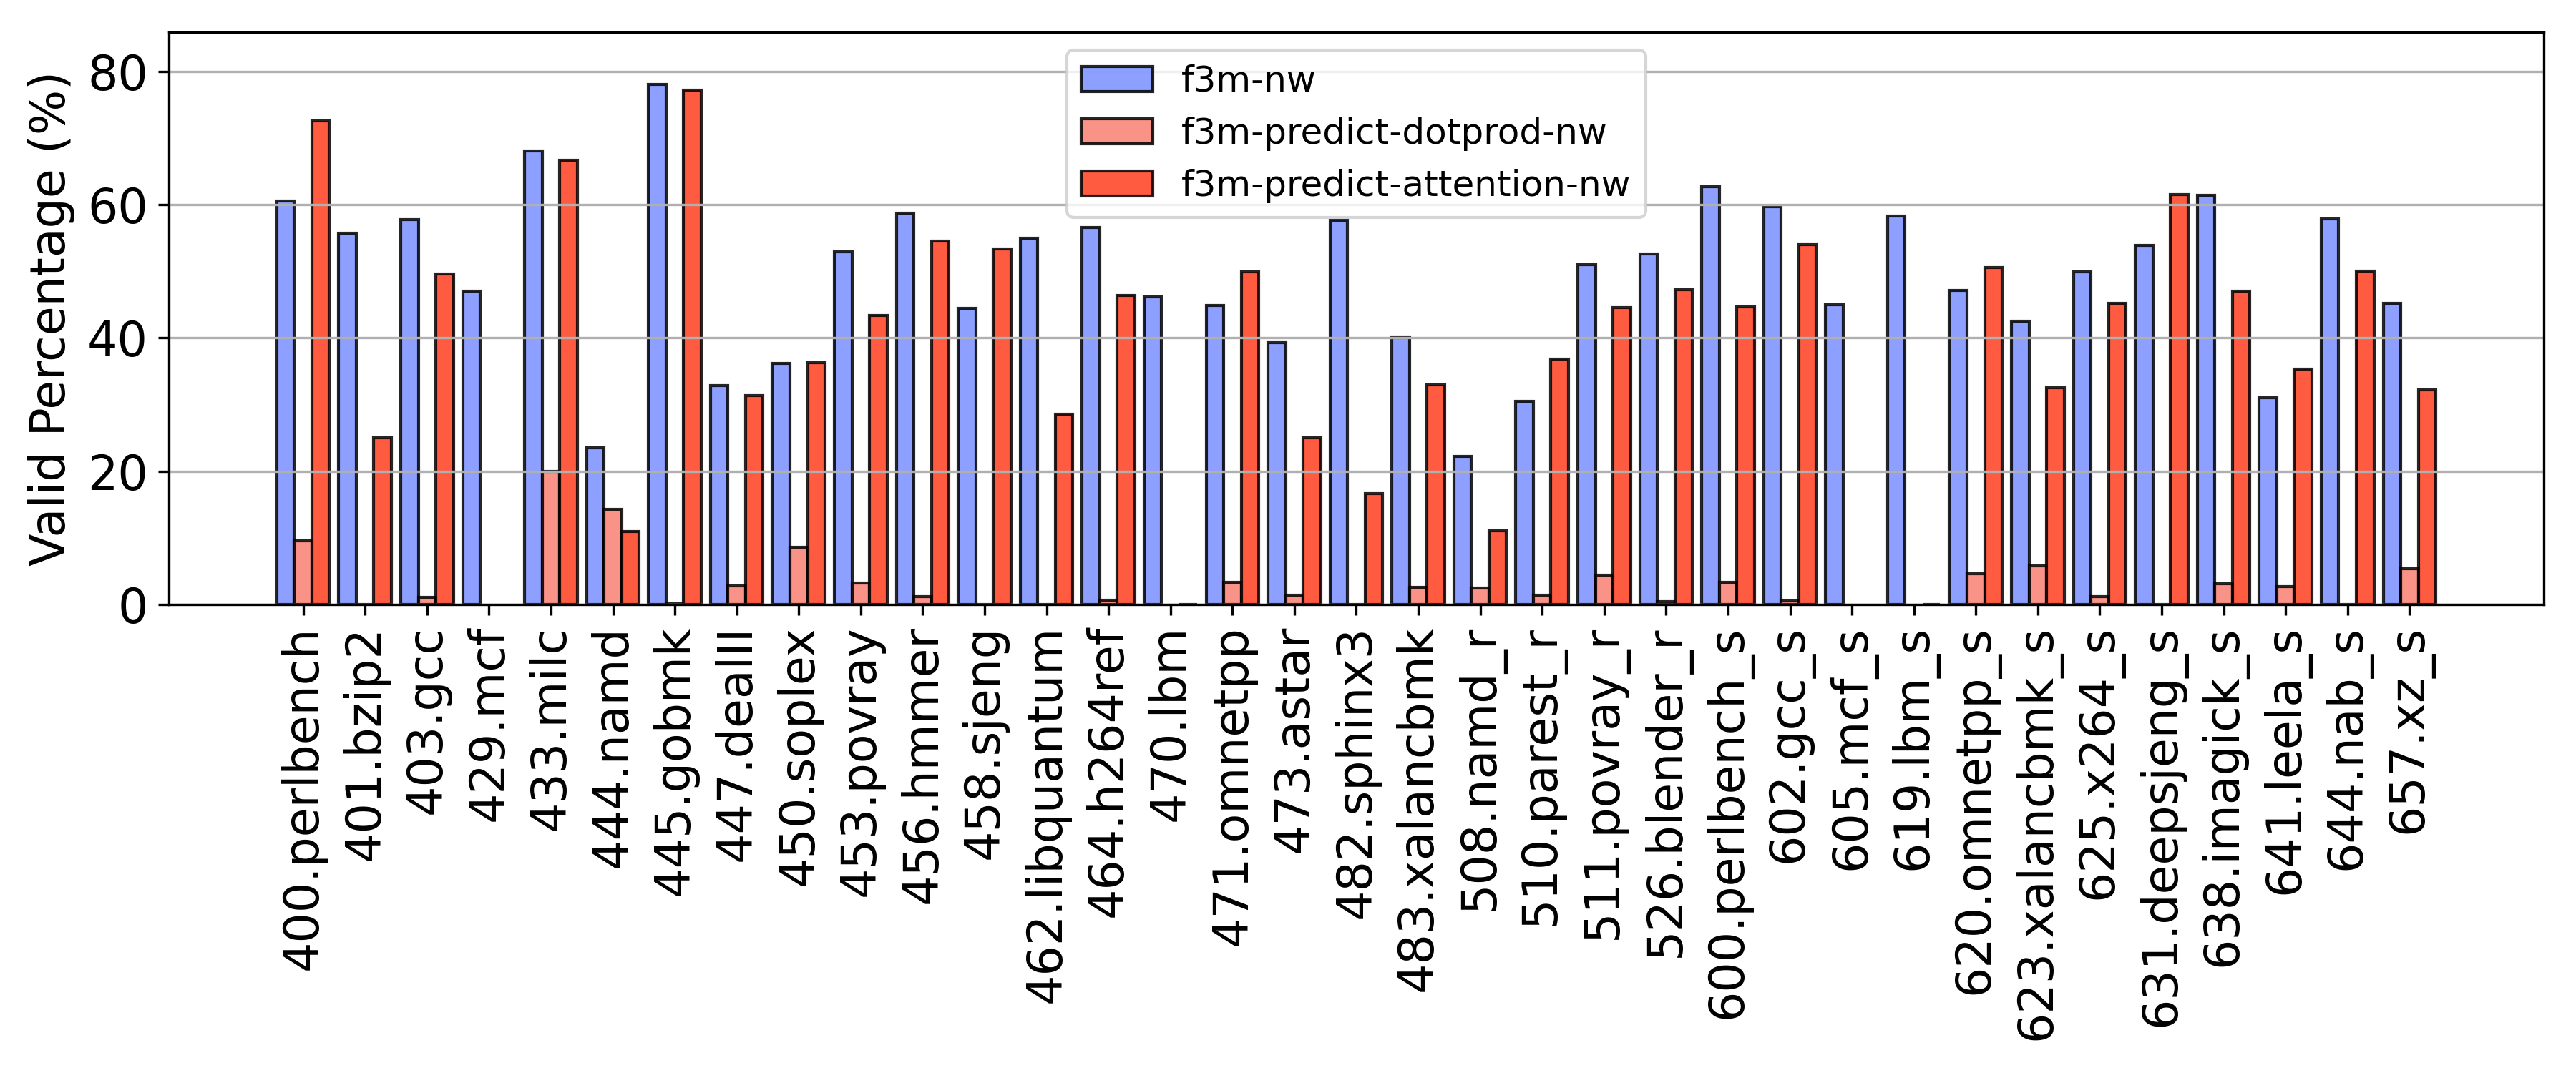
\includegraphics[scale=0.47]{Figures/Valid_Merging_Predictions/0.4_ValidPercentage.png}
%         \caption{\textbf{Ratio of Valid Merges (\textbf{0.4} Threshold)}} 
%         \label{fig:0.4Valid}
%     \end{subfigure}
%     \begin{subfigure}{\textwidth}
%         \centering
%         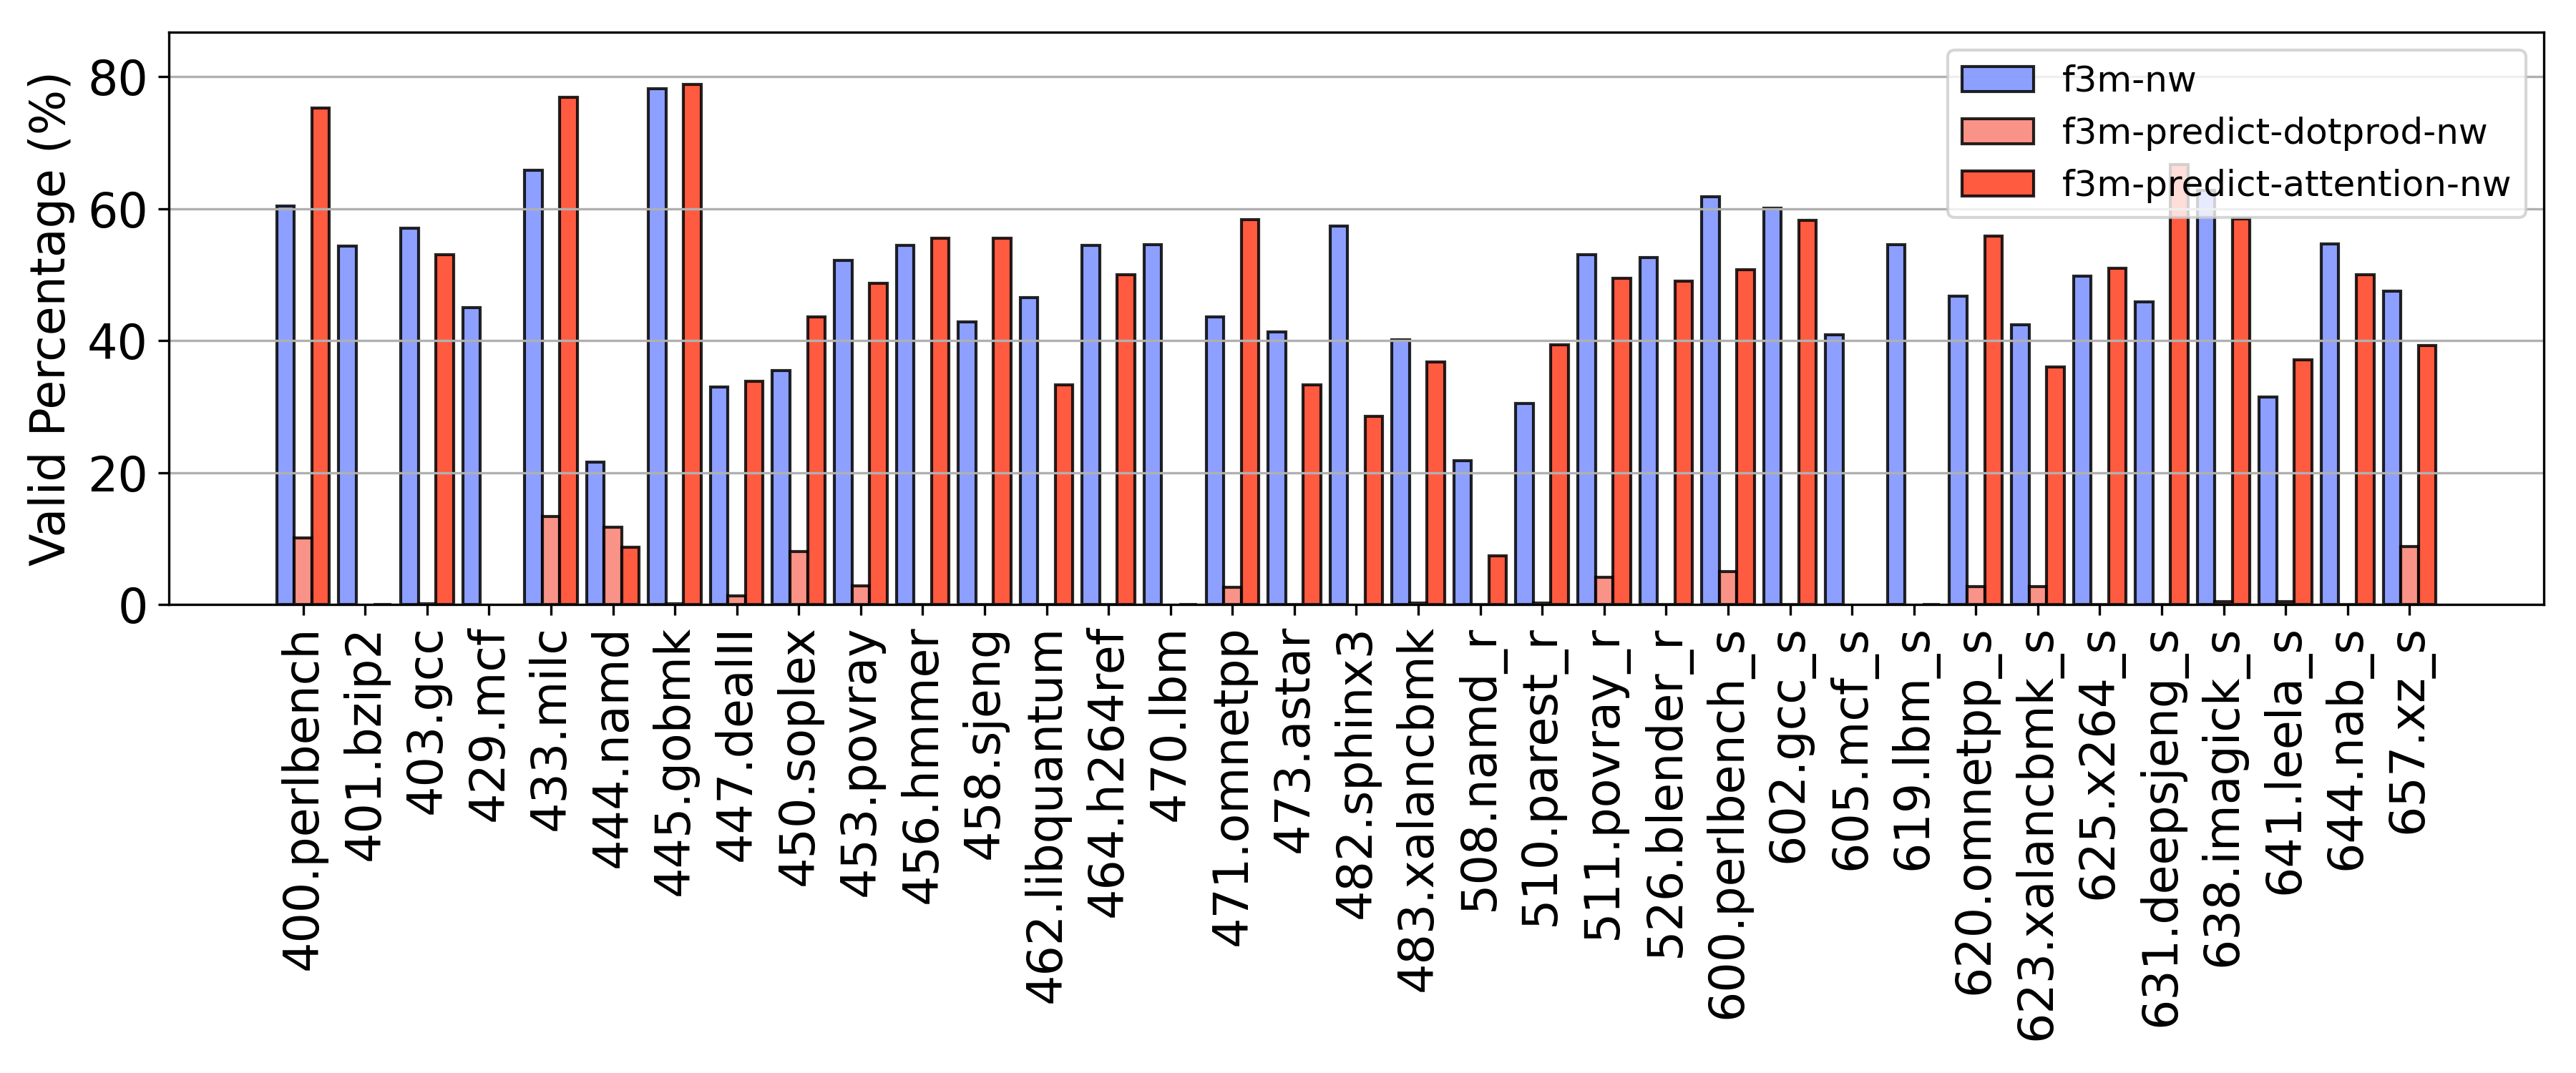
\includegraphics[scale=0.47]{Figures/Valid_Merging_Predictions/0.5_ValidPercentage.png}
%         \caption{\textbf{Ratio of Valid Merges (\textbf{0.5} Threshold)}} 
%         \label{fig:0.5Valid}
%     \end{subfigure}
%     \begin{subfigure}{\textwidth}
%     \centering
%         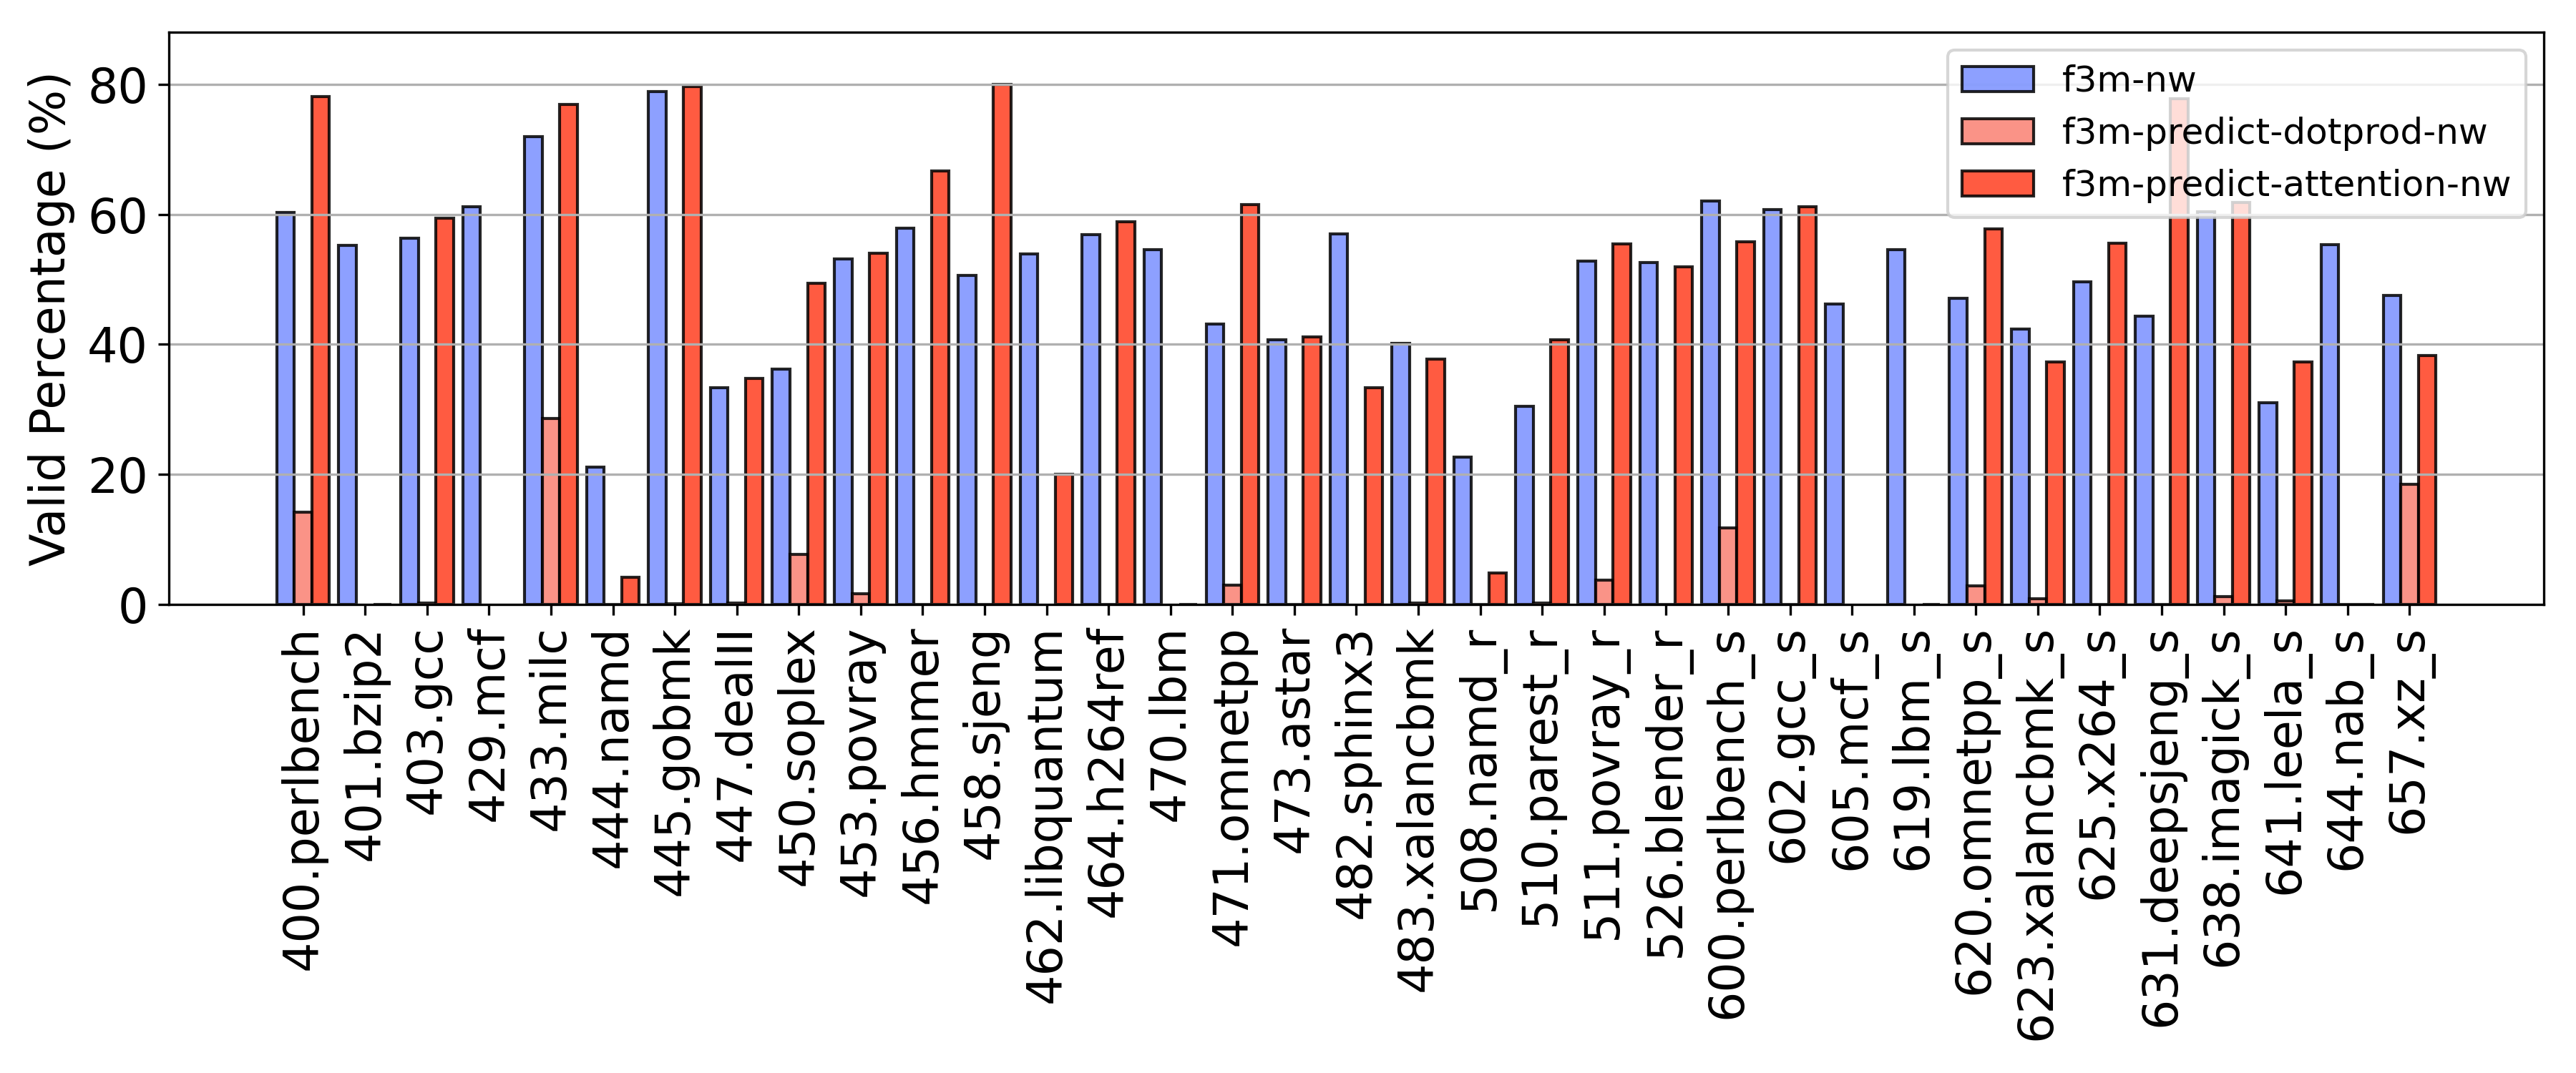
\includegraphics[scale=0.47]{Figures/Valid_Merging_Predictions/0.6_ValidPercentage.png}
%         \caption{\textbf{Ratio of Valid Merges (\textbf{0.6} Threshold)}} 
%         \label{fig:0.6Valid}
%     \end{subfigure}

%     \caption{\textbf{Percentage of Attempted Merges that are Valid.} This graph shows the proportion of merge attempts resulting in valid function pairs, calculated using equation \ref{METRIC:ValidPercentage}.} 
%     \label{fig:Valid}
% \end{figure}

% Looking at all three figures, we can quickly determine that the dot product approach fails to reliably predict valid function pairs that are suitable for merging regardless of the threshold value, struggling to break the 10\% mark in most cases. The attention model, by contrast, demonstrates considerably better ability to pick out function pairs that produce valid merges, showing an inverse relationship between the threshold and the validity percentage. This improvement is likely due to higher thresholds filtering out function pairs that the model is not confident about. At a threshold of 0.4, the attention model underperforms compared to F3M in most benchmarks (only 7 out of 35 meeting or exceeding F3M), while at 0.5 the model approximately matches F3M's performance on average (13 out of 35 benchmarks). At 0.6, the attention model outperforms F3M in the majority of cases (20 out of 35 benchmarks).

% \subsection{Profitability of Valid Merges}
% Finally, figure \ref{fig:ValidProfitable} graphs the percentage of valid merges that produced a profitable merged function. Profitability is determined when the estimated size of the newly merged function is smaller than the sum of the estimated sizes of the original function pair.

% \begin{figure}[tbh!]
%     \centering
%     \begin{subfigure}{\textwidth}
%         \centering
%         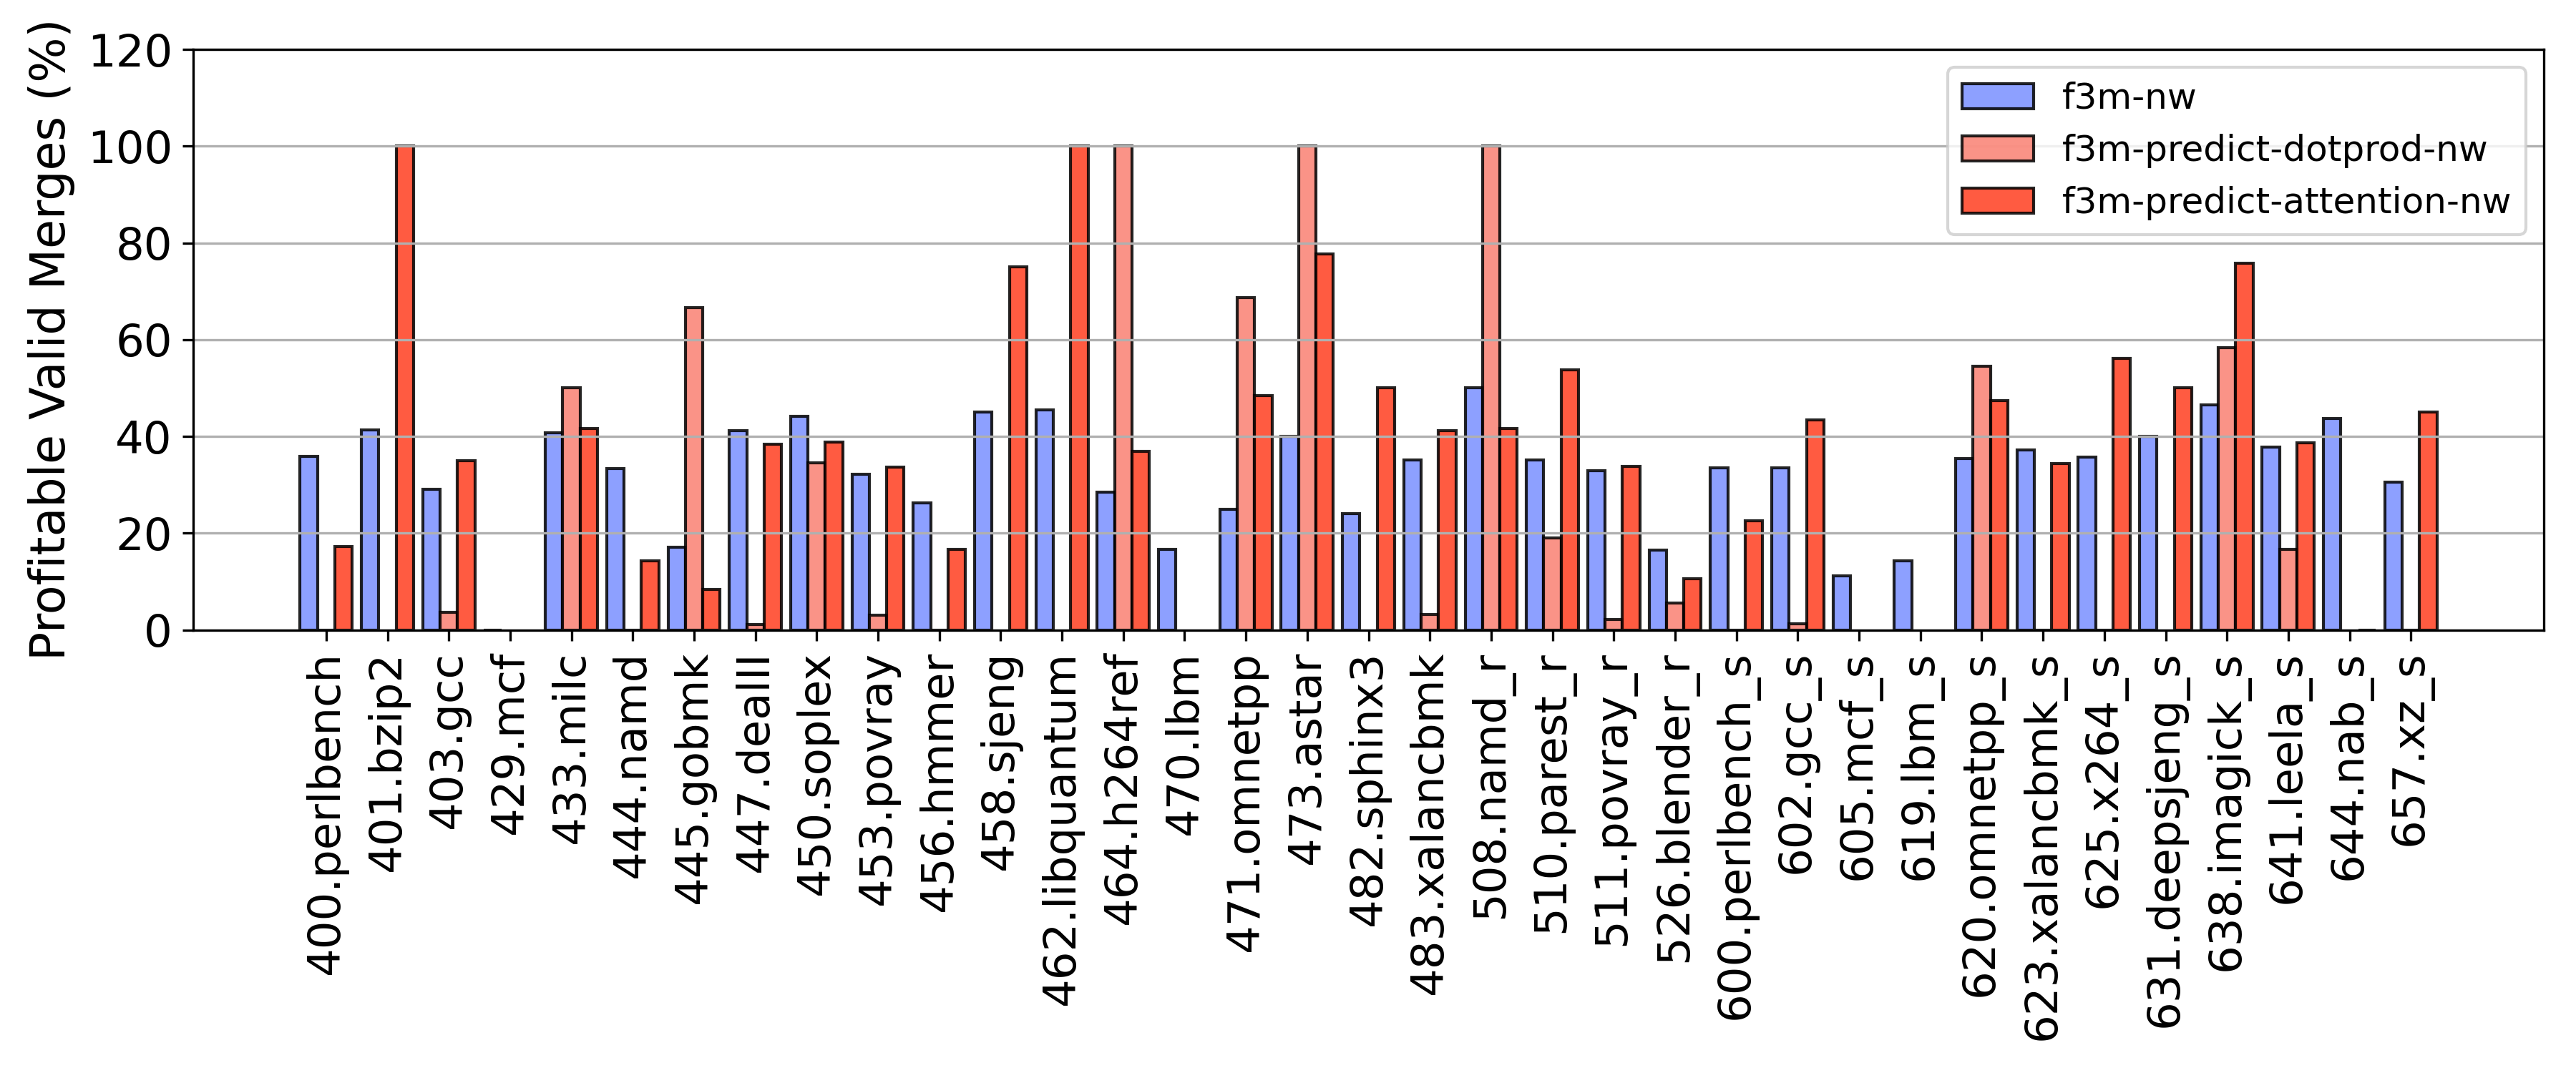
\includegraphics[scale=0.47]{Figures/Valid_Merging_Predictions/0.4_ValidProfitablePercentage.png}
%         \caption{\textbf{Profitable Valid Merges (\textbf{0.4} Threshold)}} 
%         \label{fig:0.4ValidProfitable}
%     \end{subfigure}
%     \begin{subfigure}{\textwidth}
%         \centering
%         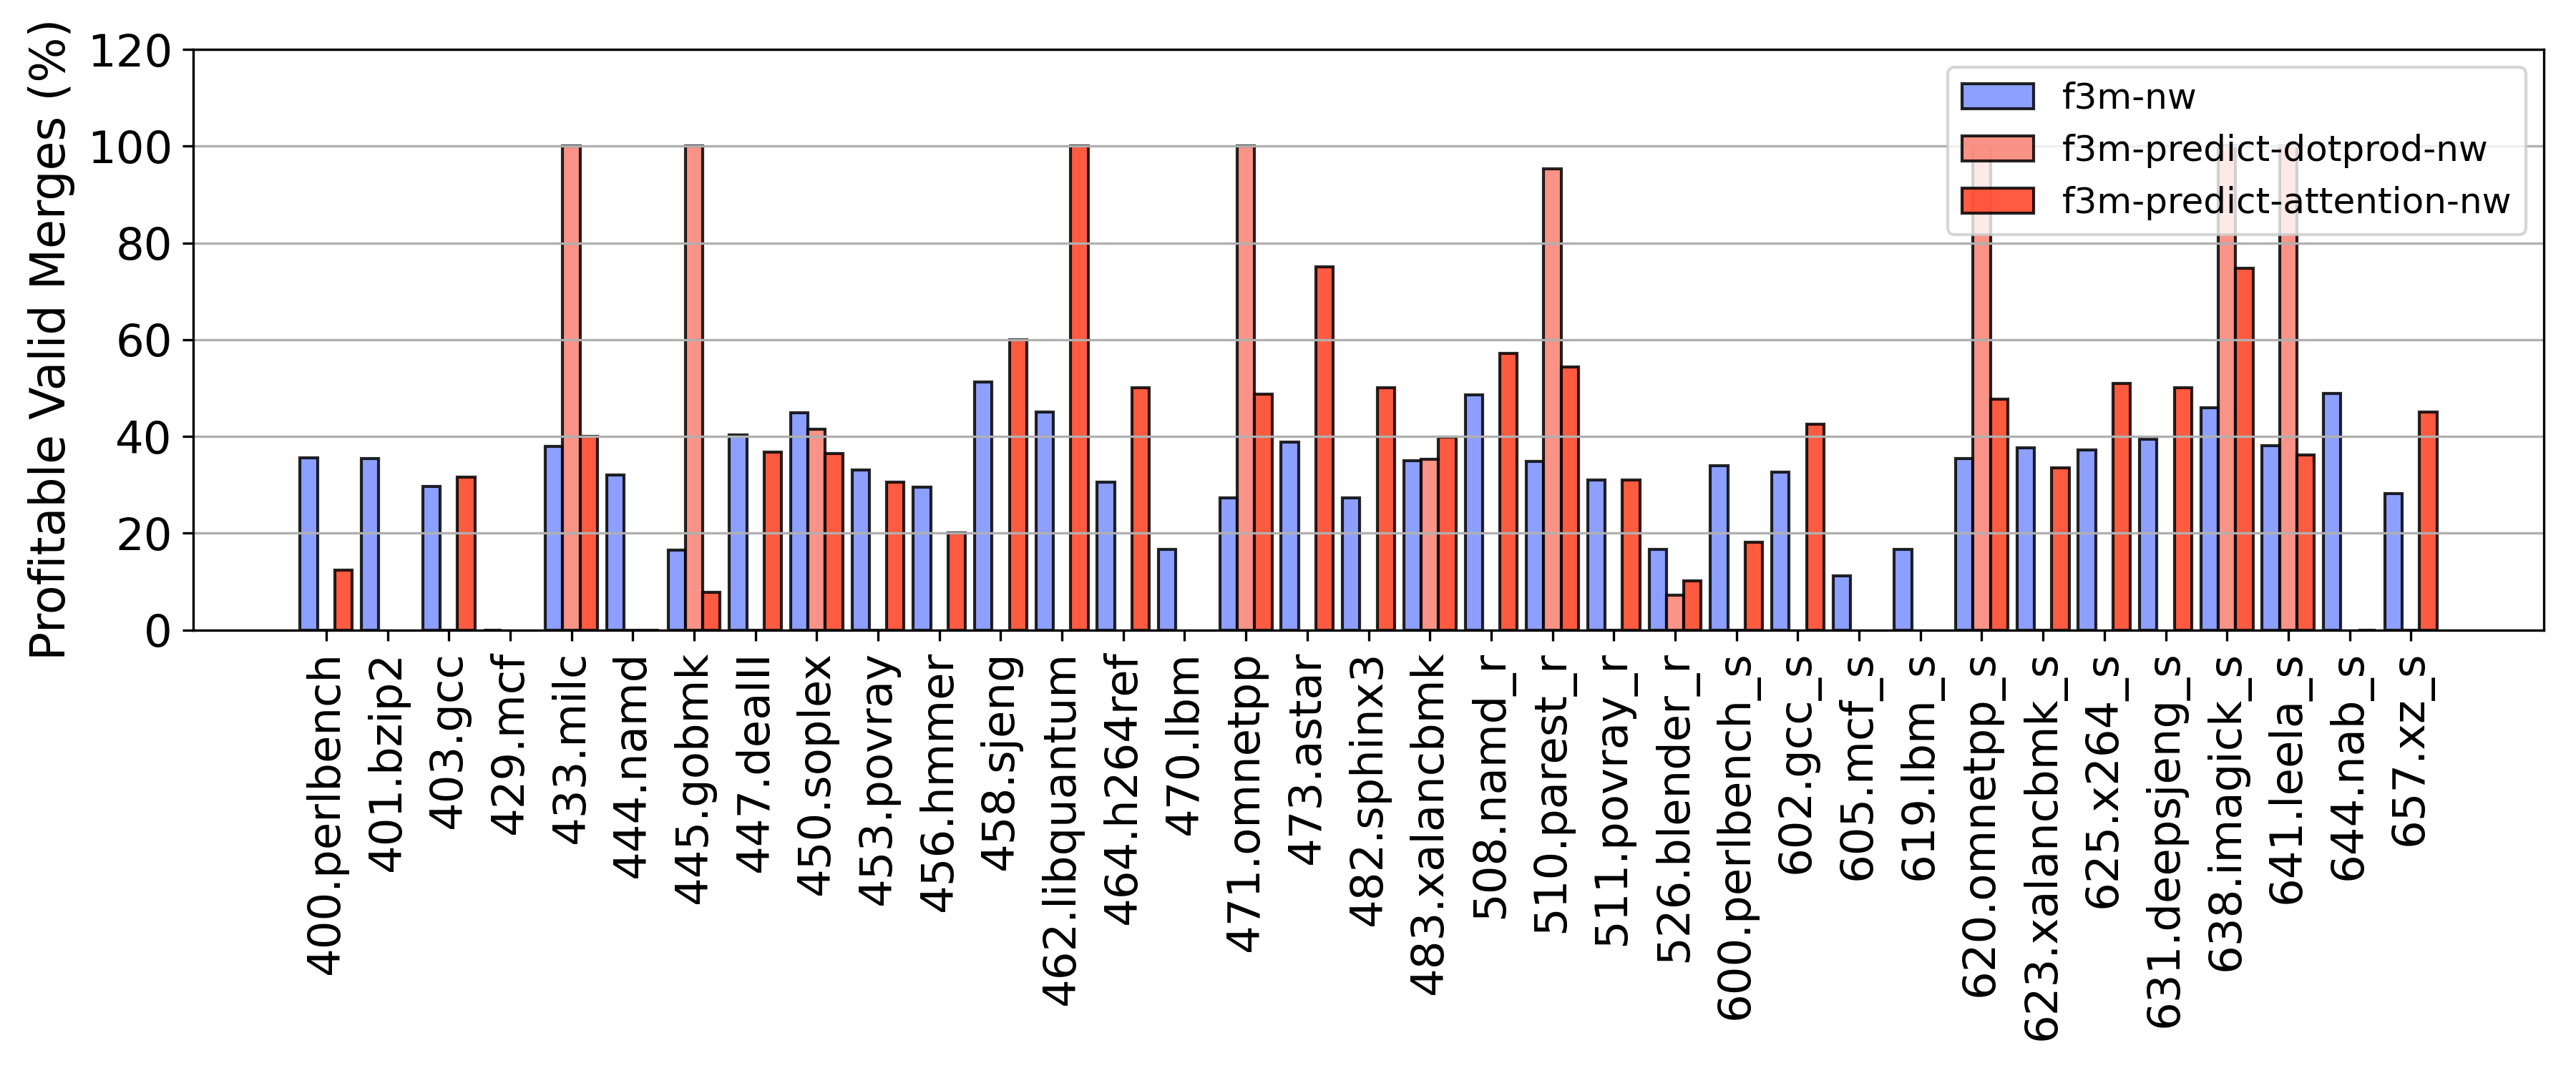
\includegraphics[scale=0.47]{Figures/Valid_Merging_Predictions/0.5_ValidProfitablePercentage.png}
%         \caption{\textbf{Profitable Valid Merges (\textbf{0.5} Threshold)}} 
%         \label{fig:0.5ValidProfitable}
%     \end{subfigure}
%     \begin{subfigure}{\textwidth}
%     \centering
%         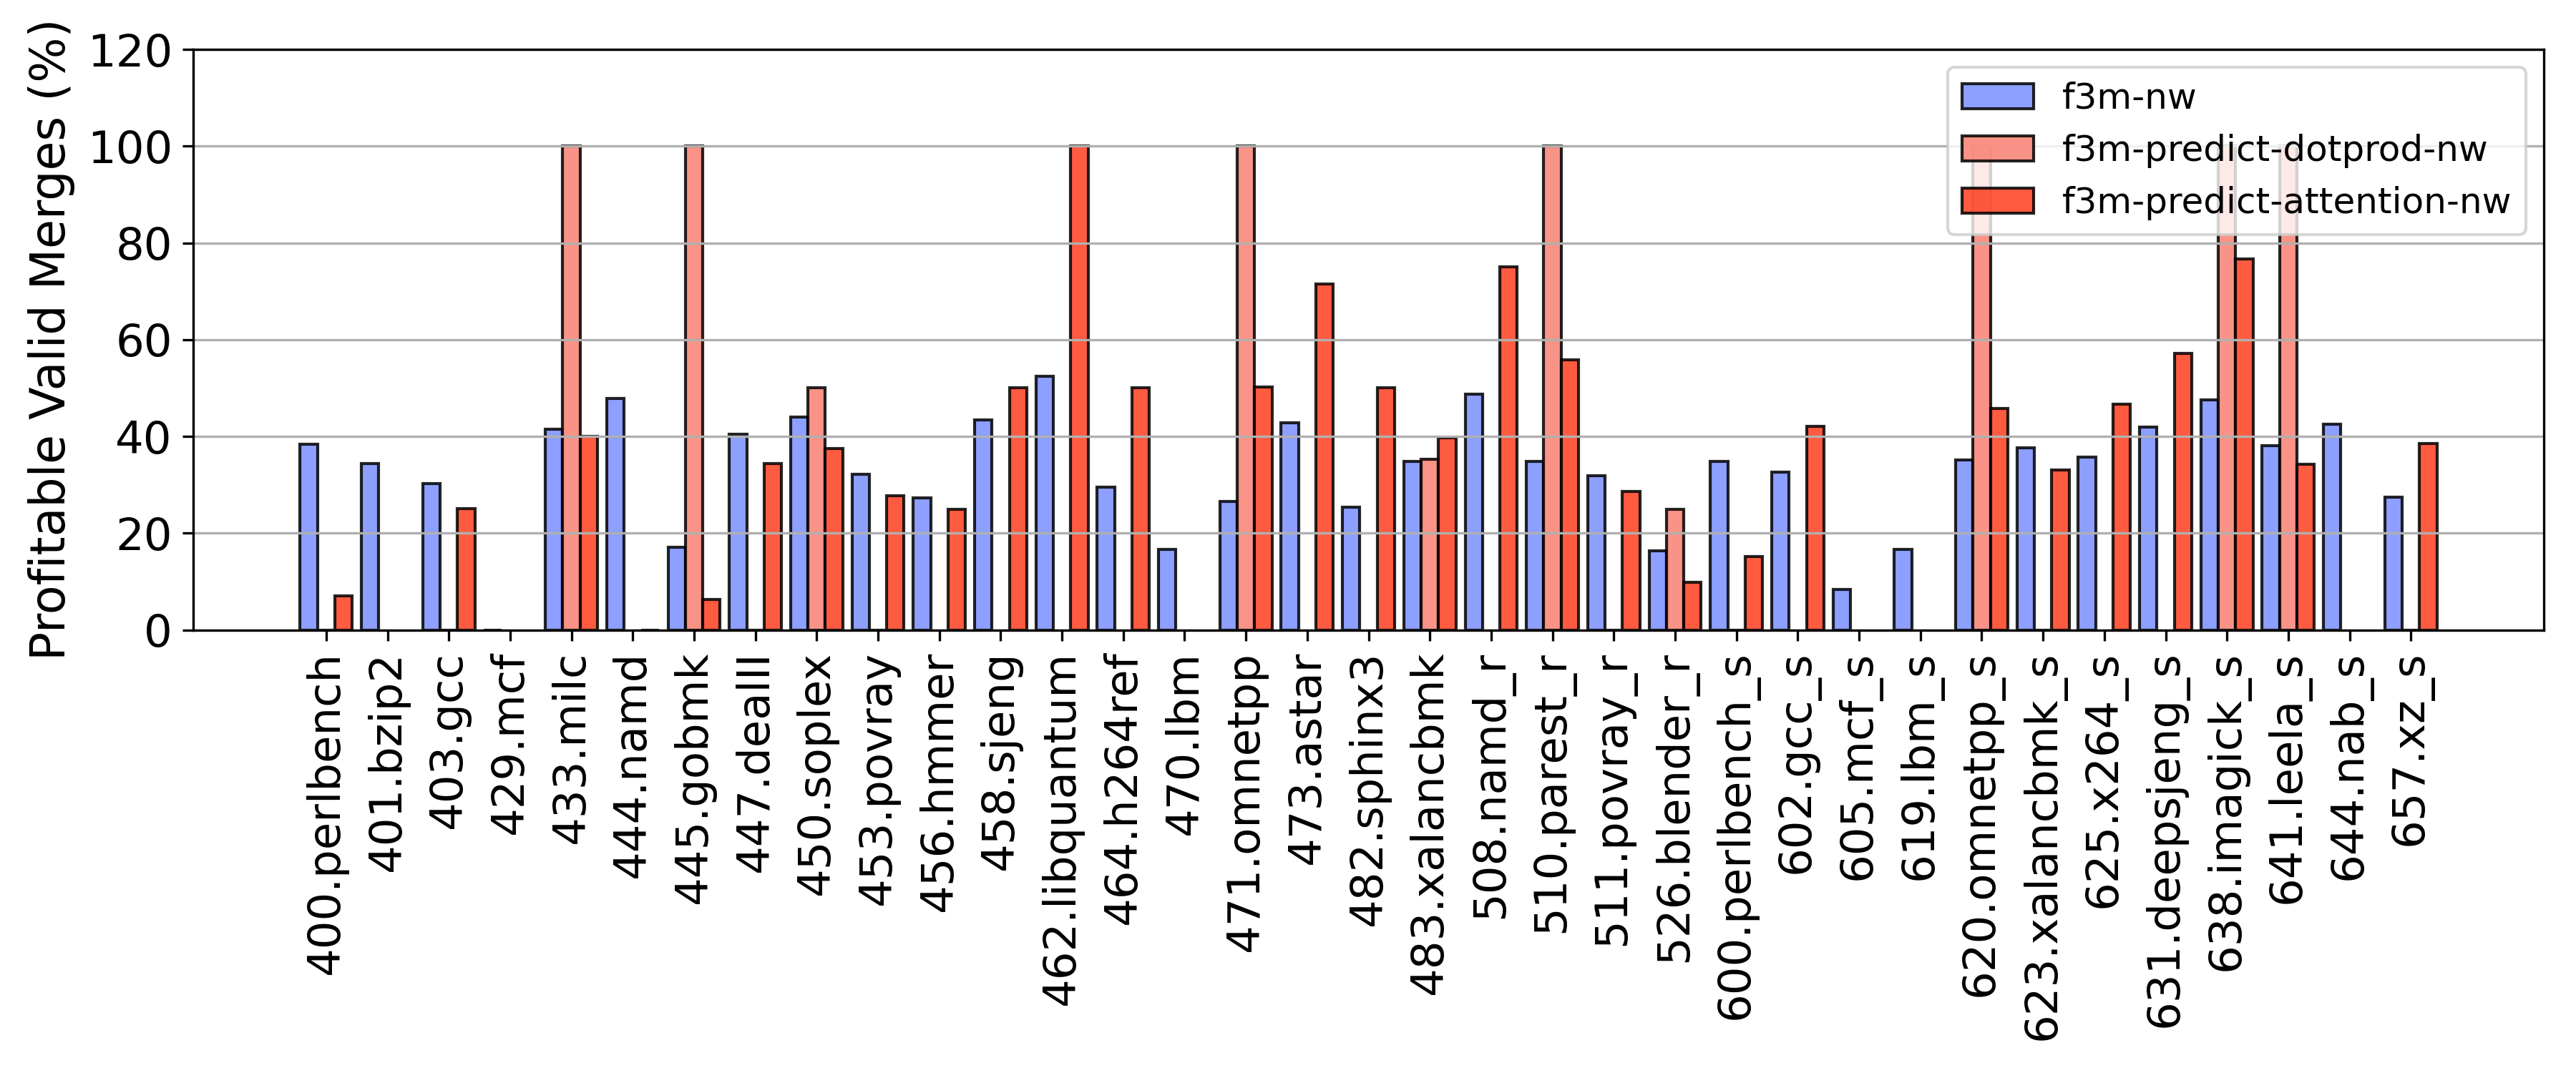
\includegraphics[scale=0.47]{Figures/Valid_Merging_Predictions/0.6_ValidProfitablePercentage.png}
%         \caption{\textbf{Profitable Valid Merges (\textbf{0.6} Threshold)}} 
%         \label{fig:0.6ValidProfitable}
%     \end{subfigure}

%     \caption{\textbf{Percentage of Valid Merges that are Profitable.} This graph illustrates the proportion of valid merges that result in code size reduction, calculated using equation \ref{METRIC:ValidProfitablePercentage}.} 
%     \label{fig:ValidProfitable}
% \end{figure}


% When comparing the performance of our different approaches across benchmarks, the prediction-based approaches generally outperform the baseline F3M across most benchmarks, with these performance differences remaining fairly consistent across all thresholds. However, exceptions exist, particularly with benchmark 401.bzip2, where the baseline outperforms both prediction models in all thresholding.

% The dot product model exhibits the most distinctive behaviour, showing the highest peaks on several benchmarks reaching 100\% profitable valid merges. Yet this approach demonstrates considerable instability, oscillating between exceptional and poor performance with few benchmarks exhibiting moderate results. Most importantly, these impressive profitability percentages must be interpreted with caution due to the dot product model's significantly lower valid function merge count. When a model finds very few valid merges to begin with, even if most of them are profitable, the absolute benefit may be minimal compared to approaches that find more valid merge candidates.
% In contrast, the attention model shows a more consistent and reliable pattern. It produces more profitable merges compared to F3M regardless of threshold, also achieving 100\% valid-profitability rates in certain phases, but crucially maintains a higher count of valid function merges. This balance makes the attention model more practical, as it wastes less computational resources by identifying a substantial number of merge opportunities while still maintaining high profitability rates.

% \subsection{Evaluation}
% The Dot Product Model demonstrates significant limitations as a heuristic for function merging. Despite occasionally proposing more merges than F3M at a 0.4 threshold and matching its volume at 0.5, its precision remains unacceptably low, topping out at only 29\% valid merges on the 433.milc benchmark at a 0.6 threshold. This indicates that over 70\% of its attempted merges are invalid and cannot produce merge-able function pairs, representing substantial wasted computational effort during compilation. Although the model reports a deceptively high profitable‑to‑valid ratio, this metric is undermined by an exceedingly small pool of valid candidates rather than by robust predictive power, rendering it an unreliable indicator of overall effectiveness for the model's performance.

% The Attention Model presents a more conservative approach than F3M, generating significantly fewer merge attempts than F3M, sometimes less than half as many. This reduction raises two possible interpretations, either the model fails to identify viable merging opportunities that F3M captures or achieves superior global optimisation by prioritising the most beneficial merges first, leaving fewer similar functions available for subsequent merges. This progressive improvement in validity suggests that higher thresholds effectively filter out invalid merge candidates at the expense of the volume of merging attempts.

% When profitability is considered, the Attention Model maintains consistent performance across all tested thresholds when measuring the ratio of attempted merges that yield profitable outcomes (17/35 benchmarks matching or exceeding F3M at every threshold), underscoring its stable precision across score cut‑offs. However, the proportion of valid merges that are profitable exhibits an inverse relationship with the threshold, performing best at 0.4 (20/35 benchmarks) and declining at higher thresholds (14/35 at 0.6). This suggests that while higher thresholds improve validity prediction, they may be overly conservative in identifying profitable merging opportunities, potentially excluding borderline cases that could yield modest but worthwhile code size reductions. In practice, a balance must be struck between the ratio of merging validity and valid-profitable merges by tuning the threshold.

% The evidence indicates that the Attention Model substantially outperforms the Dot Product Model as a function merging heuristic. Despite its high proposal volume, the Dot Product approach suffers from a poor invalid merge rate (over 70\%). In contrast, the Attention Model delivers a noticeably better balance of validity and profitability, particularly around a 0.5 threshold, where it matches or exceeds F3M's performance. Although its conservative proposal strategy may miss merge opportunities that F3M identifies, this could reflect a more globally optimal merge ordering rather than the omission of opportunities. Further evaluation is needed to determine whether the Attention Model's reduced attempt count represents optimality or overlooks merges.

% While both prediction models demonstrate superior precision in selecting profitable merging candidates when they succeed in finding valid pairs, the attention model's combination of reasonable valid merge counts and high profitability makes it the more promising approach for real-world compiler optimisation scenarios.


% \todo{Choose 0.5 seems to be the best, because it is able to balance the number }
% \todo{Mention that mcf is quite small, so functionmerging is not done for most of it. So should consider a total of 34 instead of 35 benchmarks???}


% \todo{Attention Model does not seem to be able to pick out options from a small pool of functions, it tensds to work better when given a large pool of functions: Validity}.


\section{Code Size Reduction} \label{Eval:CodeSizeReduction}
Lastly, we analyse the effect the three approaches, F3M, Dot Product Predictions and Attention Predictions, have on code size reduction compared to LLVM's default compiled binary. There are two metrics this evaluation focuses on, the size of the compiled-code segment of the binary file (also known as \textit{.text}) and the size of the binary file (\textit{binary size}). The compiled-code section of an executable contains only the actual machine code instructions, holding the code that will be executed at runtime. The binary size, on the other hand, refers to the total size of the compiled file. This includes all the machine code instructions, global variables, read-only data, and other metadata specific to the executable format. The compiled-code section size provides direct insight into the effectiveness of function merging optimisation, while the binary size allows us to understand the overall impact on the executable size.

% Since F3M employs heuristics with randomised components, it is not deterministic. It was executed three times to account for this variability, and the average result was calculated. The deep learning approach, which predicts alignment scores between function pairs using IR2Vec embeddings, aims to achieve better code size reduction than F3M.

\subsection{Compiled-Code Segment Size Reduction}
Figures \ref{fig:DotTextSizeComparison} presents the compiled-code section size reduction achieved by the three function merging approaches (F3M, Dot Product Predictions, and Attention Predictions) across the benchmark suite compared to the baseline LLVM compilation. This metric is particularly relevant as it isolates the impact on actual executable code size, allowing us to evaluate each method's capability to identify and merge similar functions while excluding other factors that may affect the overall binary size.


\begin{figure}[tbh!]
    \centering
    \begin{subfigure}{\textwidth}
        \centering
        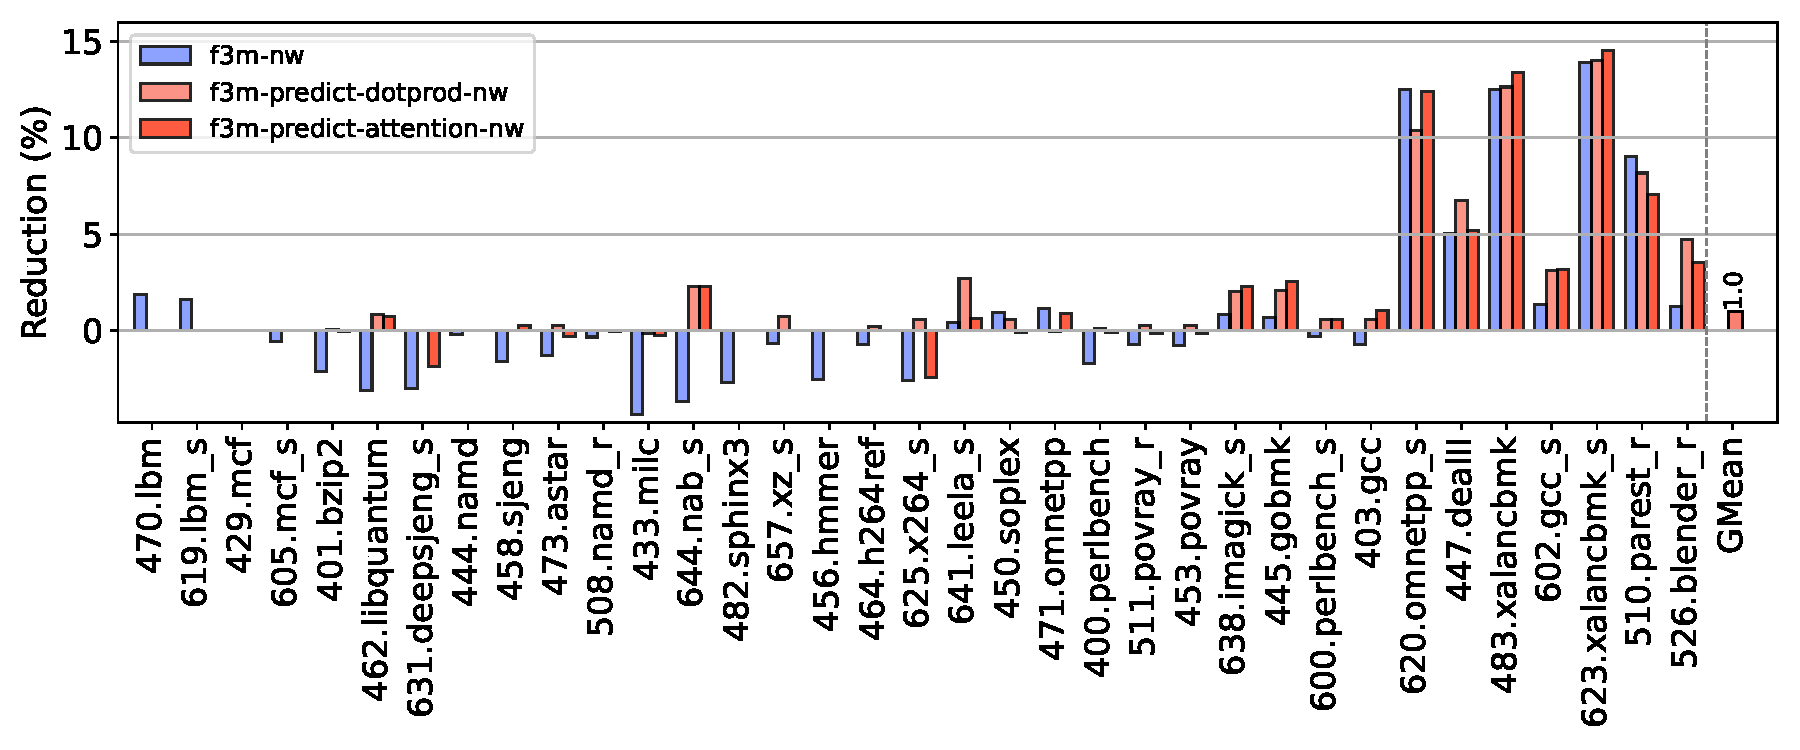
\includegraphics[scale=0.47]{Figures/CodeSizeAnalysis/0.4_dottext_code-size-reduction.pdf}
        \caption{Dot Text Size Reduction with \textbf{0.4} Threshold)}
        \label{fig:0.4BinSizeCodeSize}
    \end{subfigure}
    \begin{subfigure}{\textwidth}
        \centering
        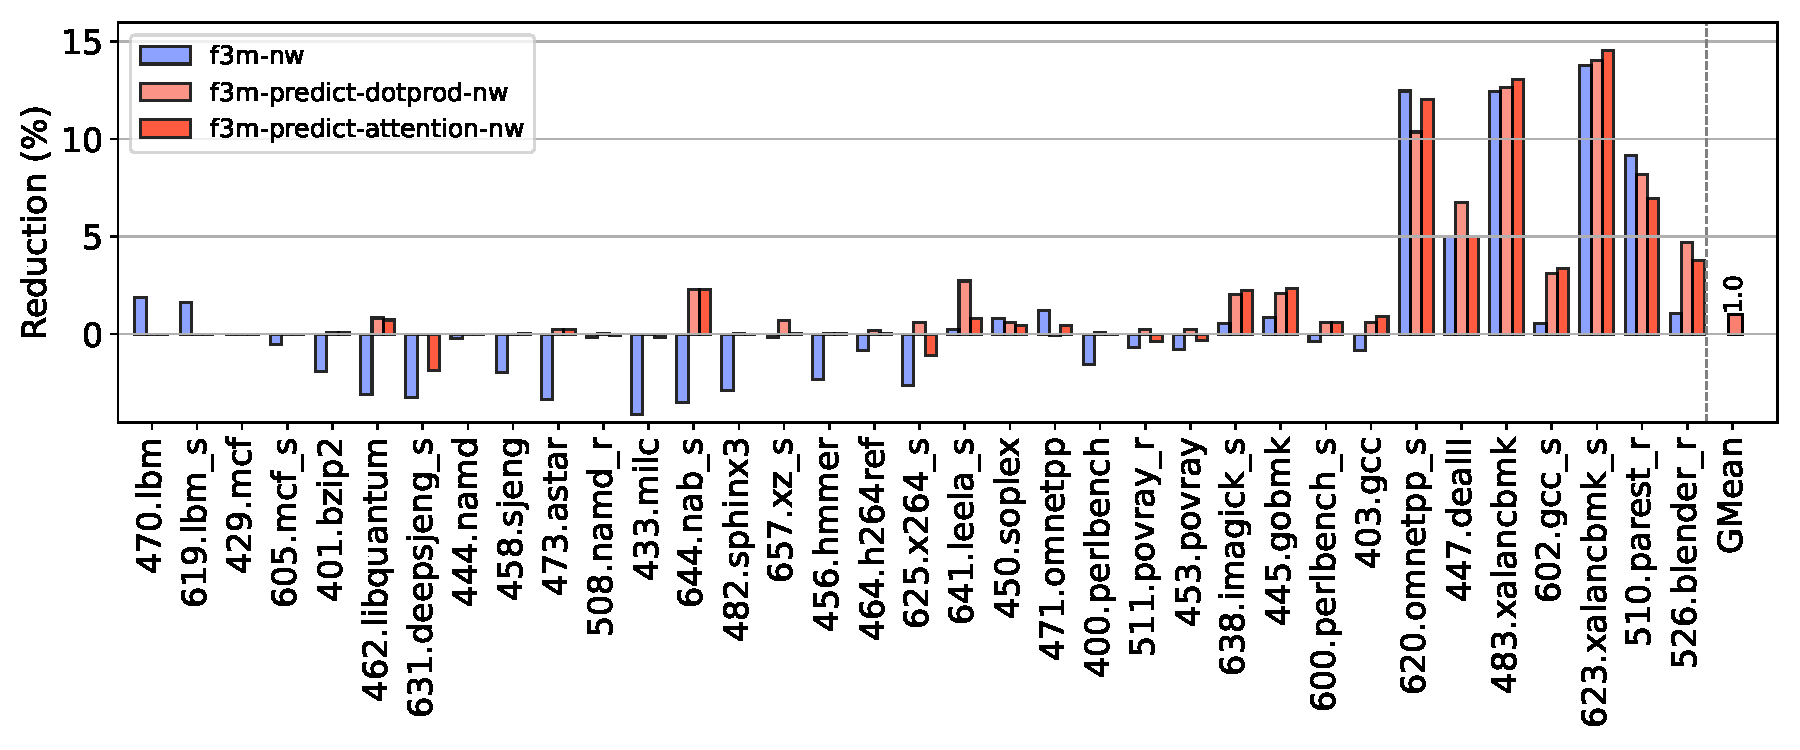
\includegraphics[scale=0.47]{Figures/CodeSizeAnalysis/0.5_dottext_code-size-reduction.pdf}
        \caption{Dot Text Size Reduction with \textbf{0.5} Threshold)}
        \label{fig:0.5BinSizeCodeSize}
    \end{subfigure}
    \begin{subfigure}{\textwidth}
    \centering
        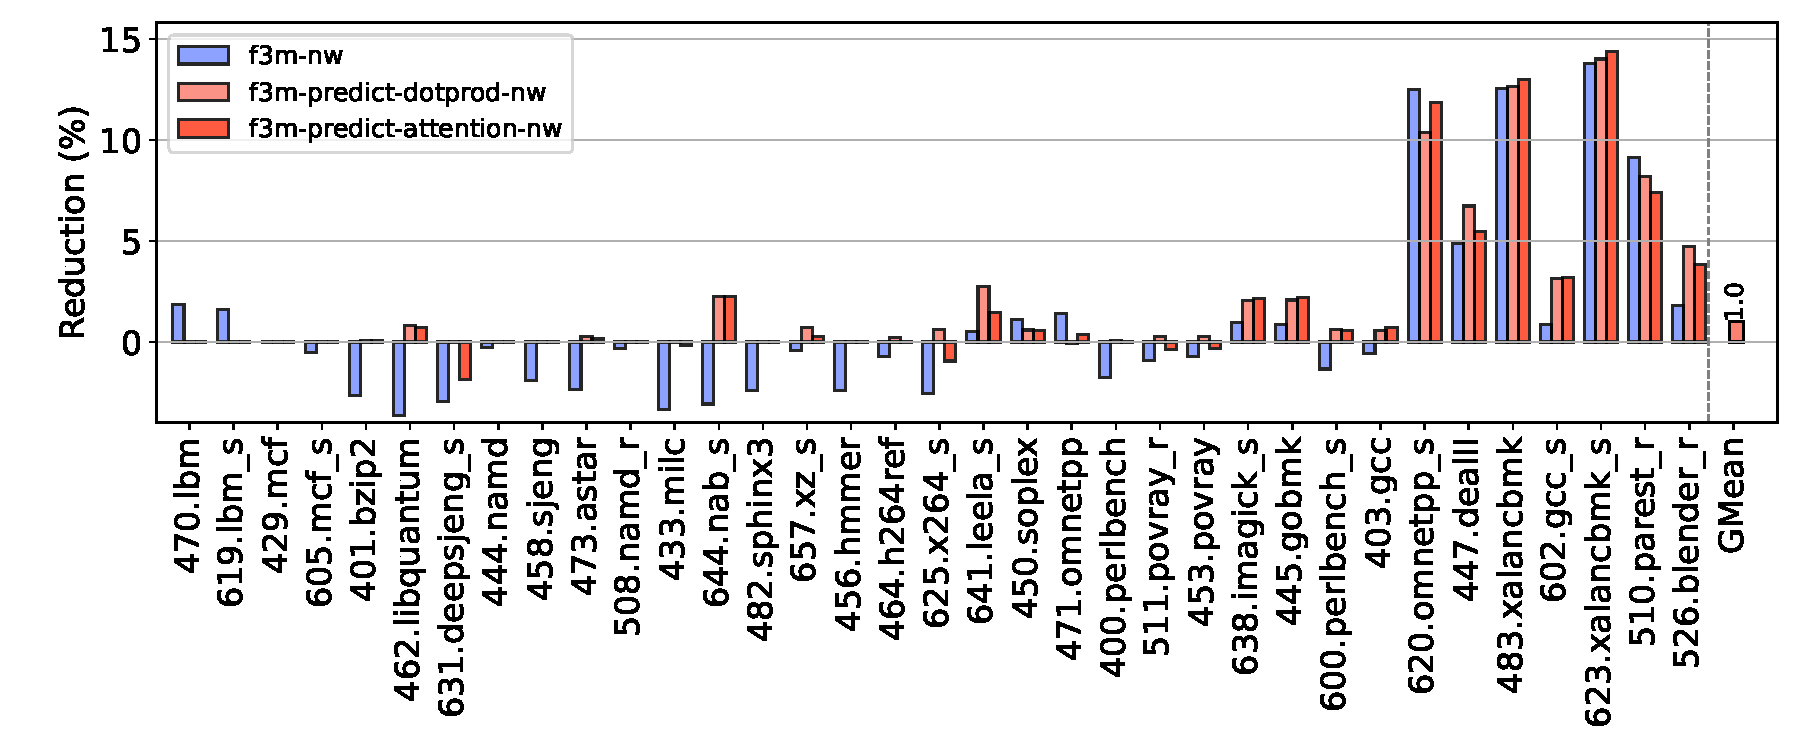
\includegraphics[scale=0.47]{Figures/CodeSizeAnalysis/0.6_dottext_code-size-reduction.pdf}
        \caption{Dot Text Size Reduction with \textbf{0.6} Threshold)}
        \label{fig:0.6BinSizeCodeSize}
    \end{subfigure}

    \caption{\textbf{Dot Text Size Reductions Across Different Thresholds.} The percentage of dot text size reduction is shown against the baseline, which is the default LLVM without any experimental function merging (Higher is better).}
\label{fig:DotTextSizeComparison}
\end{figure}

F3M achieved an average compiled-code section size reduction of \textbf{2.9}\% across SPEC CPU 2006 and SPEC CPU 2017 benchmarks, while our machine learning-based approaches demonstrated superior performance with reductions of \textbf{4.4}\% and \textbf{4.2}\% for the Dot Product and Attention models respectively. This represents a significant improvement of approximately 50\% over the state-of-the-art F3M technique.

While examining individual benchmark performance, F3M consistently outperformed our predictive models on four benchmarks (450.soplex, 471.omnetpp, 620.omnetpp\_s, and 510.parest\_r) across all threshold configurations. However, our predictive approaches demonstrated greater consistency in reducing the compiled-code segment size, particularly on smaller benchmarks where F3M frequently increased the size rather than reduced it.

Regarding threshold sensitivity, the Dot Product model showed identical performance at thresholds of 0.5 and 0.6, with minimal difference when lowered to 0.4. The Attention model exhibited even more stable behaviour, with reduction percentages ranging narrowly from 4.24\% to 4.29\% across different thresholds. This shows that the threshold does not play a significant role in the compiled-code section's size at the granularity of thresholds we assessed.

% Both the Dot Product and Attention model significantly surpassed F3M's capabilities, demonstrating that our machine learning approach successfully captures function similarities that traditional heuristic-based methods miss.

In summary, both the Dot Product and Attention model frequently surpassed F3M's capabilities, demonstrating that our machine learning approach successfully captures function similarities that traditional heuristic-based methods miss.

\subsection{Binary Size Reduction}
The binary size reduction provides a more comprehensive view of optimisation impact, capturing potential overheads in metadata, branch tables, and other sections that might be introduced during function merging. This metric is important for evaluating real-world deployment scenarios where total storage requirements matter. Figures \ref{fig:binSizeComparison} show the overall binary size reduction achieved by our three function merging approaches across SPEC2006 and SPEC2017 benchmarks compared to the baseline default LLVM compilation. 

\begin{figure}[tbh!]
    \centering
    \begin{subfigure}{\textwidth}
        \centering
        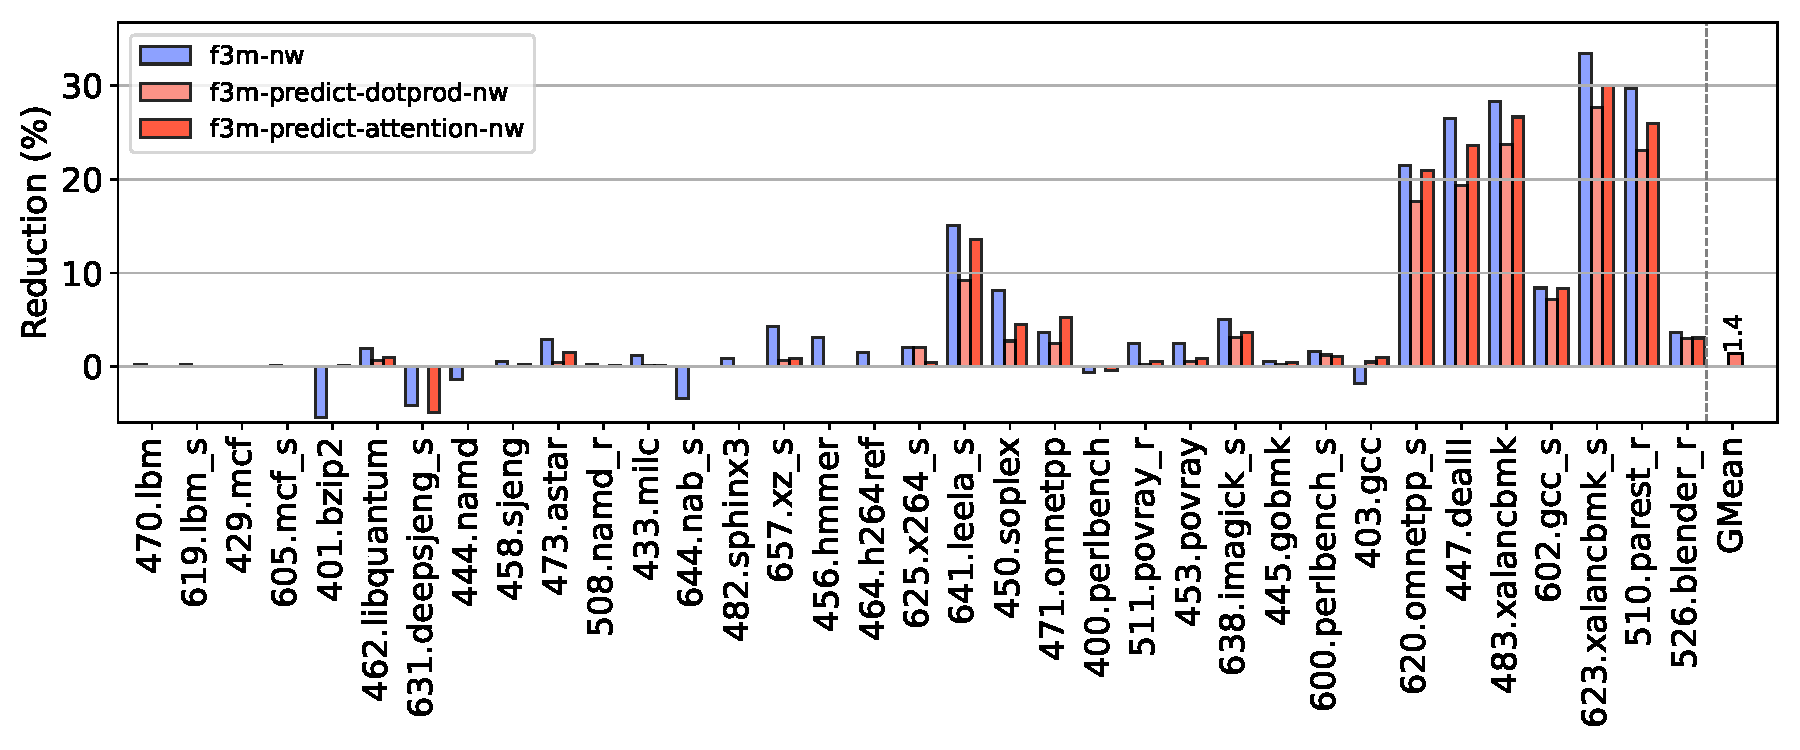
\includegraphics[scale=0.47]{Figures/CodeSizeAnalysis/0.4_binsize_code-size-reduction.pdf}
        \caption{\textbf{Binary Size Reduction (\textbf{0.4} Threshold)}} 
        \label{fig:0.4BinSizeCodeSize}
    \end{subfigure}
    \begin{subfigure}{\textwidth}
        \centering
        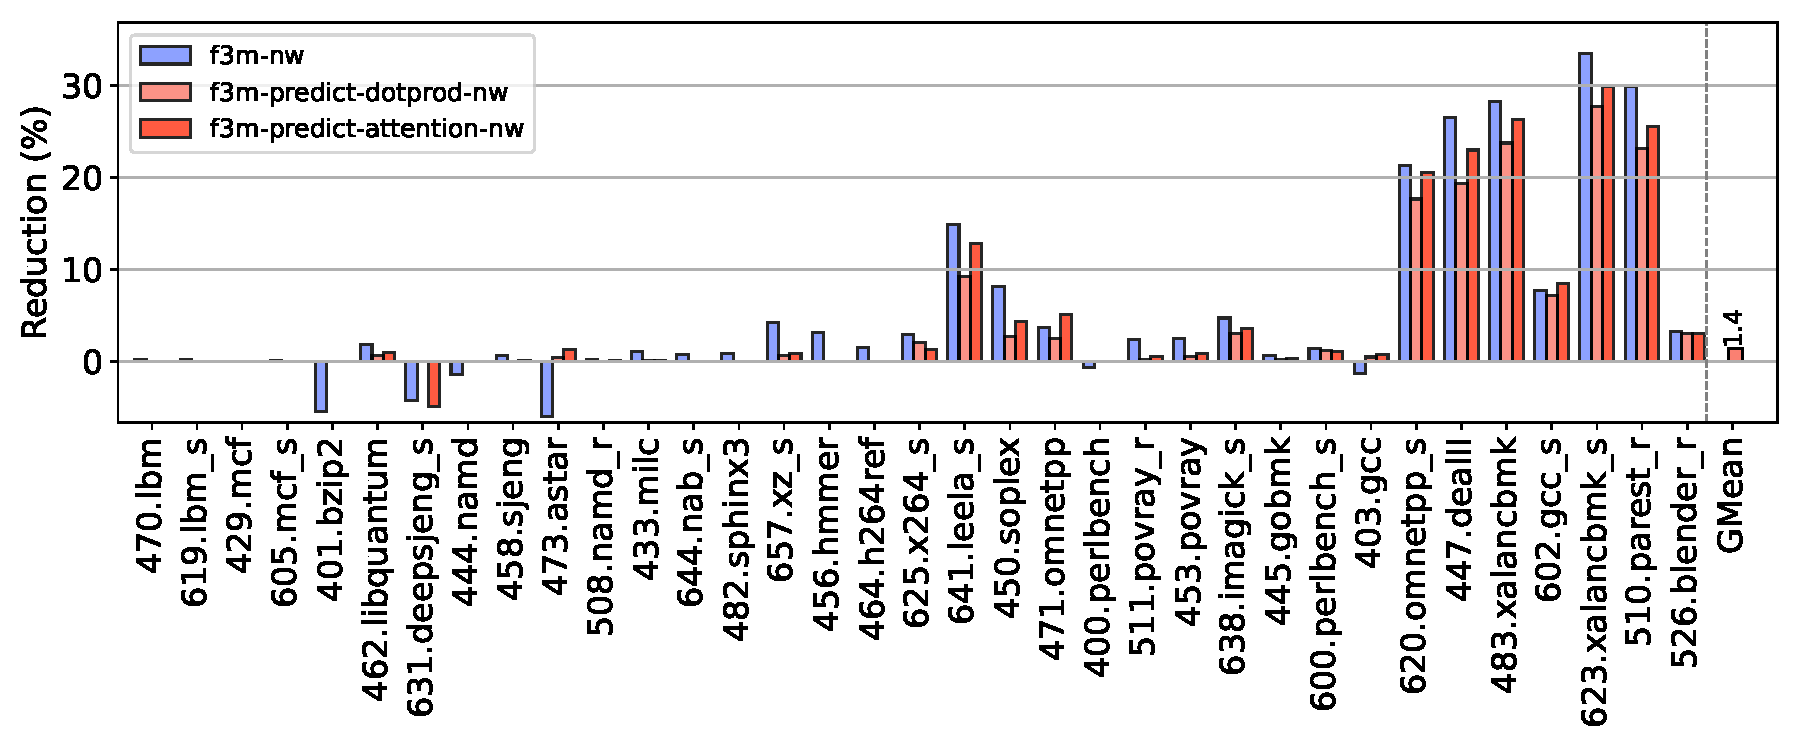
\includegraphics[scale=0.47]{Figures/CodeSizeAnalysis/0.5_binsize_code-size-reduction.pdf}
        \caption{\textbf{Binary Size Reduction (\textbf{0.5} Threshold)}} 
        \label{fig:0.5BinSizeCodeSize}
    \end{subfigure}
    \begin{subfigure}{\textwidth}
    \centering
        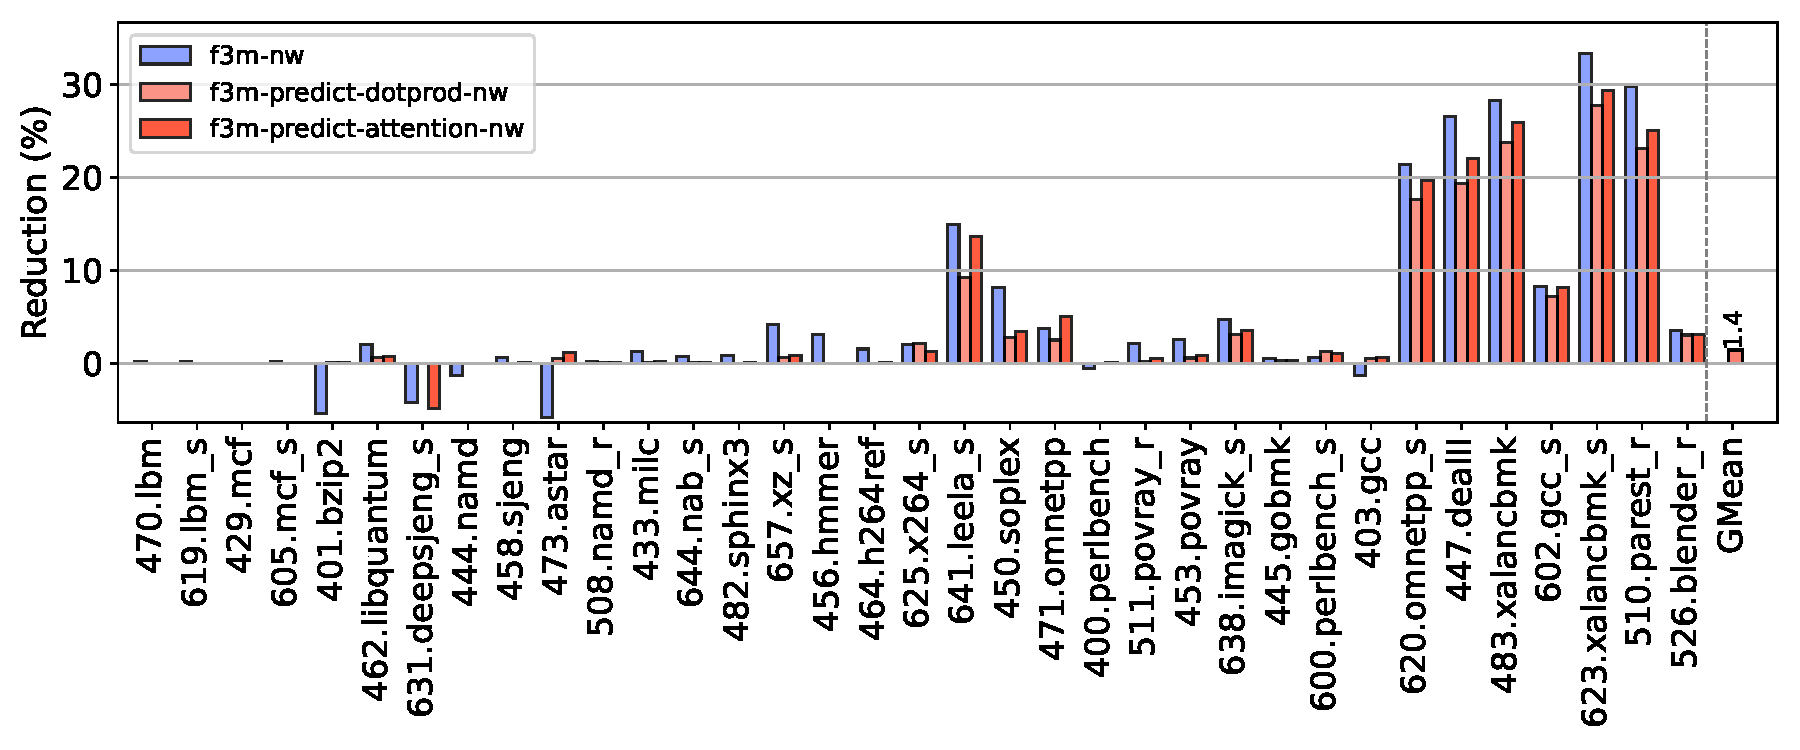
\includegraphics[scale=0.47]{Figures/CodeSizeAnalysis/0.6_binsize_code-size-reduction.pdf}
        \caption{\textbf{Binary Size Reduction (\textbf{0.6} Threshold)}} 
        \label{fig:0.6BinSizeCodeSize}
    \end{subfigure}

    \caption{\textbf{Binary Size Reductions Across Different Thresholds.} The percentage of binary size reduction is shown against the baseline, which is the default LLVM without any experimental function merging (Higher is better).}
\label{fig:binSizeComparison}
    \label{fig:binSizeComparison}
\end{figure}

Unlike the compiled-code segment size results, figure \ref{fig:binSizeComparison} reveals the traditional F3M approach maintains an edge in overall binary optimisation, achieving a substantial \textbf{12.1\%} reduction across our benchmark suite. Our machine learning techniques demonstrated respectable but lesser reductions of \textbf{9.9\%} (Dot Product) and \textbf{11\%} (Attention), suggesting F3M's heuristics may better address factors beyond code sections that influence total executable size. The Attention model was able to show promising results on three benchmarks (\textit{471.omnetpp}, \textit{403.gcc}, and \textit{602.gcc\_s}), where it outperformed F3M across all threshold configurations.

The predictability of our ML-based approaches stands as their most compelling advantage. The Dot Product model exhibited remarkable consistency, producing zero adverse outcomes across all benchmarks, a guarantee against unwanted size increases that F3M cannot provide. Similarly, the Attention model triggered negative reduction in just one case (\textit{631.deepsjeng\_s}), vastly outperforming F3M's unpredictable behaviour on smaller benchmarks. In comparison, F3M increased binary size on multiple smaller benchmarks, making our approaches more reliable for size-sensitive applications.

Threshold configuration analysis revealed minimal sensitivity across both models. The Attention implementation showed slightly better performance at lower thresholds (ranging from 10.7\% to 11.1\% reduction), but the practical difference remains negligible for most deployment considerations. The Dot Product model's results across all thresholds are almost identical, further emphasising this stability.

\subsection{Evaluation}
None of the implementations could make a breakthrough with both mcf benchmarks, regardless of threshold, likely because there are no possible merges. Despite this limitation, both predictive models showed promising results when examining how effectively machine learning can eliminate redundant code.

If we look at the compiled-code section size reduction, the predictive approach worked better than F3M, showing approximately 50\% improvement. This metric best demonstrates the effects of function merging on code. It indicates superior performance compared to the previous state-of-the-art, representing a significant improvement for both predictive models. Surprisingly, the dot product approach performs well despite its poor merging prediction quality, functioning similarly to F3M by helping shortlist functions for the compiler to attempt merges.

While the predictive models work quite well, with their ability to decrease binary size, they fall slightly behind F3M, representing a 13\% decrease in reduction compared to F3M, but do keep it in mind that this reduction was achieved without any hand-crafted heuristic used to decide the function merges.

One reason for this discrepancy can be attributed to the data stored for exception handling. The exception handling frame (.eh\_frame section) stores the call frame information (CFI), which describes how to restore the stack state at any point in program execution, necessary for stack unwinding during exception propagation. The exception handling frame header (.eh\_frame\_hdr section) is used for binary searching into the exception handling frame during runtime to quickly locate the appropriate frame description entry for a given program counter value, optimising exception handling.

When functions are merged, the CFI must maintain precise stack unwinding instructions for each possible execution path through the merged function. This requires additional CFI directives to track stack unwinding information across multiple execution paths that previously existed in separate functions. The merged function must maintain all exception-handling capabilities of the original functions while managing them within a single code body, leading to a substantial increase in exception metadata despite the reduction in code size.

The exception handling frame for the dot product and attention models are 13.6\% and 8.5\% larger than F3M's and 11.7\% and 6.9\% larger for the exception handling frame header. This shows an inverse relationship between the amount of compiled-code size and the exception-handling metadata. This demonstrates how function merging can lead to smaller compiled-code sections but larger overall binaries due to this metadata expansion.

If users are willing to take a slight risk when running function merging, it is better to use the attention model than dot product because the binary size will likely be smaller if the code size is reduced, though there is a slight chance that the size will increase slightly. On the other hand, dot product is safer, much less likely to generate a larger size for both the compiled-code section and binary size, but the reduction is less aggressive. Performance is also left on the table since the merged functions were not considered for merging again due to IR2Vec's versioning issues. 

The compile time for the dot product and attention model approaches are 10 and 23 times longer than F3M. This is due to the implementation where the alignment score is predicted between a function and all other functions before merging with the highest aligned function. This process is costly and could benefit from a multi-tiered analysis process where earlier stages prune off non-profitable functions.
\chapter{Conclusion - 10\%}


\section{Future Work}

\begin{itemize}
    \item Try reinforcement learning instead
    \item Try a different type of embedding?
\end{itemize}

\bibliography{refs}    % this causes the references to be listed

\bibliographystyle{plain}
%% the bibliography style determines the format  in which both citations and references are printed,
%% other possible values are plain and abbrv
%%
%% If you want more control of the format of your citations you might want to take a look at
%% natbib.sty, which should be part of any standard LaTeX installation
%%
%% University regulations simply require that your citation style be consistent, so see what style
%% your supervisor recommends.

% Appendices start here

\appendix
\chapter{Appendix}
\section{Acronyms}

\begin{center}
\begin{tabular}{ |c|c| } 
 \hline
 \textbf{Acronym} & \textbf{Full-Form} \\ 
 \hline
 CFG & Control-Flow Graph \\ 
 ML & Machine Learning \\
 F3M & Fast Focused Function Merging\\
 MSE & Mean Squared Error\\
 MAE & Mean Absolute Error\\
 MAPE & Mean Absolute Percentage Error\\
 IR & Intermediate Representation\\
 IOT & Internet of Things\\
 SOTA & State-of-the-Art \\
 \hline
\end{tabular}
\end{center}

\end{document}
